% 第四章 群: 再次相遇 --- 中译
% 原书 pp. 171--236 (Aluffi, Algebra: Chapter 0, Chapter IV).
% 本文件进度: §\ref{sec:conjugation}--§\ref{subsec:sylow} 已译 (2026-08-29); §\ref{sec:composition-solvability} 以下待续.

\chapter{群:再次相遇}
\label{chap:groups2}

在本章中, 我们回到 $\cate{Grp}$, 研究若干比第二章所考虑的内容``更不一般''的课题. 我们在这里所做的大部分内容将专门适用于有限群; 这本身就是一个重要的例子, 因为它有着辉煌的应用 (例如在 Galois 理论中; 参见 \S VII.\ref{sec:galois-applications}), 而且从叙述的角度看它也是一个好题材, 因为它使我们有机会看到几个一般概念在一个足够复杂以承载实质内容、又足够简单以易于领会 (就这一小撮初等课题而言) 的语境中发挥作用.

\section{共轭作用}
\label{sec:conjugation}

\subsection{群在集合上的作用: 回顾}
\label{subsec:actions-reminder}

当你让群作用在什么东西上时, 群才真正大放异彩. 本节将非常有效地证明这一点, 因为通过对 \S~II.\ref{subsec:transitive-actions} 中建立的关于群作用的初等事实进行极其头脑简单的应用, 我们将得到关于有限群的出奇精确的结果.

回顾我们证明过 (命题~II.\ref{prop:transitive-orbits}): 群 $G$ 在集合 $S$ 上的每个传递的 (左) 作用, 在相差自然同构概念的意义下, 都是``在左陪集之集 $G/H$ 上的左乘''. 这里 $H$ 可以取为任意元素 $a \in S$ 的稳定子 $\Stab_G(a)$, 即 (定义~II.\ref{def:stabilizer}) 固定 $a$ 的 $G$ 的子群. 这一事实适用于 $G$ 在一个集合上的每个左作用的轨道; 特别地, 有限轨道 $O$ 中元素的个数等于 $O$ 中任意 $a$ 的稳定子的指数; 特别地 (推论~II.\ref{cor:orbit-divides}), 若 $G$ 有限, 则轨道的元素个数 $|O|$ 必须整除 $G$ 的阶 $|G|$.

这些考虑可以打包成一个有用的``计数''公式, 对那个作用我们可以称之为类公式%
\index{leigongshi@类公式(class formula)}
; 这个名字通常保留给 $G$ 通过共轭作用于自身的特殊情形, 我们将在下文更仔细地探讨它.

为陈述该公式, 设 $G$ 作用在集合 $S$ 上; 对 $a \in S$, 令 $G_a$ 表示稳定子 $\Stab_G(a)$. 再令 $Z$ 为作用的不动点之集:
\[
Z = \{a \in S \mid (\forall g \in G):\ ga = a\}.
\]
注意 $a \in Z \iff G_a = G$; 我们可以说, $a \in Z$ 当且仅当 $a$ 的轨道是``平凡的'', 意思是它仅由 $a$ 一人组成.

\begin{proposition}
\label{prop:class-formula}
设 $S$ 是有限集, $G$ 是作用在 $S$ 上的群. 沿用上面的记号,
\[
|S| = |Z| + \sum_{a \in A} [G:G_a],
\]
其中 $A \subseteq S$ 对该作用的每个非平凡轨道恰含一个元素.
\end{proposition}

\begin{proof}
轨道构成 $S$ 的一个划分, 而 $Z$ 收集了平凡的轨道; 于是
\[
|S| = |Z| + \sum_{a \in A} |O_a|,
\]
其中 $O_a$ 表示 $a$ 的轨道. 由命题~II.\ref{prop:transitive-orbits}, 阶 $|O_a|$ 等于 $a$ 的稳定子的指数, 即得所述.
\end{proof}

命题~\ref{prop:class-formula} 的主要力量在于: 若 $G$ 有限, 则每个和项 $[G:G_a]$ 整除 $G$ 的阶 (且大于 $1$). 当关于 $|G|$ 的某些信息已知时, 这可以是一个很强的约束. 比如, 看看当 $G$ 是 $p$-群时它说了什么:

\begin{definition}
\label{def:p-group}
$p$-群%
\index{pqun@p-群(p-group)}
是阶为素整数 $p$ 的幂的有限群.
\end{definition}

\begin{corollary}
\label{cor:fixed-points}
设 $G$ 是作用在有限集 $S$ 上的 $p$-群, $Z$ 是该作用的不动点之集. 则
\[
|Z| \equiv |S| \bmod p.
\]
\end{corollary}

\begin{proof}
的确, 命题~\ref{prop:class-formula} 中的每个和项 $[G:G_a]$ 都是大于 $1$ 的 $p$ 的幂; 从而它模 $p$ 为 $0$.
\end{proof}

例如, 在某些情形这可以用来确立 $Z \neq \emptyset$%
\footnote{在这个意义下, 命题~\ref{prop:class-formula} 是一类被称为``不动点定理''的结果的一个实例. 读者在拓扑学课程中多半会遇到几个这样的定理, 在那里集合的``大小''的角色可以 (比如) 由拓扑空间的 Euler 示性数来扮演.}%
: 见习题~\ref{ex:p-group-fixed}. 命题~\ref{prop:class-formula} 的这类直接推论将在下文西罗定理的证明中助我们一臂之力.

\index{gongelei@共轭类(conjugacy class)!zai $S_n$ zhong@在 $S_n$ 中(in $S_n$)}\subsection{中心、中心化子、共轭类}
\label{subsec:center-conjugacy}

回顾 (例~II.\ref{ex:left-multiplication}) 每个群 $G$ 都以至少两种有趣的方式作用于自身: 通过 (左) 乘与通过共轭%
\index{gonge@共轭(conjugation)}
. 后一作用由如下 $\rho : G \times G \to G$ 定义:
\[
\rho(g, a) = gag^{-1}.
\]
如我们所知 (\S~II.\ref{subsec:actions-sets}), 这一数据等价于某个群同态的数据:
\[
\sigma : G \to S_G,
\]
即从 $G$ 到 $G$ 上的置换群的群同态.

这个作用凸显了几个有趣的对象:

\begin{definition}
\label{def:center}
$G$ 的中心%
\index{zhongxin@中心(center)}
, 记作 $Z(G)$, 是 $G$ 的子群 $\Ker \sigma$.
\end{definition}

具体地说, $G$ 的中心\footnote{为何用 $Z$? ``中心''的德文是 Zentrum.}是
\[
Z(G) = \{g \in G \mid (\forall a \in G):\ ga = ag\}.
\]
的确, $\sigma(g)$ 是 $S_G$ 中的恒同, 当且仅当 $\sigma(g)$ 在 $G$ 上作为恒同作用; 也就是说, 当且仅当对所有 $a \in G$ 有 $gag^{-1} = a$; 也就是说, 当且仅当 $g$ 与 $G$ 的所有元素交换. 换言之, 中心是 $G$ 在共轭作用下的不动点之集.

注意, 群 $G$ 的中心自动在 $G$ 中正规: ``手工''验证这几乎是立即的, 但无需这么做, 因为按定义它是一个核, 而核是正规的.

群 $G$ 交换, 当且仅当 $Z(G) = G$, 也就是说, 当且仅当共轭作用在 $G$ 上是平凡的.

\index{guina@归纳(induction)}一般地, 当你发现一个群的中心非平凡时, 尽管高兴: 这常常使你能对群的元素个数作归纳来建立证明, 办法是模掉中心 (大致说来, 这正是我们将证明第一西罗定理的方式). 或者注意下面这个在试图证明群交换时很顺手的有用事实:

\begin{lemma}
\label{lem:quotient-center-cyclic}
设 $G$ 是有限群, 且 $G/Z(G)$ 是循环的. 则 $G$ 是交换的 (从而 $G/Z(G)$ 事实上是平凡的).
\end{lemma}

\begin{proof}
(参见习题~\ref{ex:G-Z-cyclic-inn}.) 由于 $G/Z(G)$ 循环, 存在元素 $g \in G$ 使得类 $gZ(G)$ 生成 $G/Z(G)$. 那么 $\forall a \in G$
\[
aZ(G) = (gZ(G))^r
\]
对某个 $r \in \Z$ 成立; 也就是说, 存在中心的元素 $z \in Z(G)$ 使 $a = g^r z$.

现在若 $a$, $b$ 属于 $G$, 利用这一事实写
\[
a = g^r z, \qquad b = g^s w
\]
对某个 $s \in \Z$ 与 $w \in Z(G)$ 成立; 然而
\[
ab = (g^r z)(g^s w) = g^{r+s}zw = (g^s w)(g^r z) = ba,
\]
其中我们用到了 $z$ 与 $w$ 同 $G$ 的每个元素交换这一事实. 由于 $a$ 与 $b$ 是任意的, 这证明 $G$ 交换.
\end{proof}

接下来, $a \in G$ 在共轭下的稳定子有一个特别的名字:

\begin{definition}
\label{def:centralizer}
$a \in G$ 的中心化子%
\index{zhongxinhazi@中心化子(centralizer)}
(或正规化子%
\index{zhengguihuazi@正规化子(normalizer)}
) $Z_G(a)$ 是它在共轭下的稳定子.
\end{definition}

于是,
\[
Z_G(a) = \{g \in G \mid gag^{-1} = a\} = \{g \in G \mid ga = ag\}
\]
由 $G$ 中那些与 $a$ 交换的元素构成. 特别地, 对所有 $a \in G$ 有 $Z(G) \subseteq Z_G(a)$; 事实上, $Z(G) = \bigcap_{a \in G} Z_G(a)$. 显然 $a \in Z(G) \iff Z_G(a) = G$.

若对包含 $a$ 的群 $G$ 不存在歧义, 则可省去下标 $G$.

\begin{definition}
\label{def:conjugacy-class}
$a \in G$ 的共轭类%
\index{gonggelei@共轭类(conjugacy class)}
是 $a$ 在共轭作用下的轨道 $[a]$. $G$ 的两个元素 $a$, $b$ 称为共轭的%
\index{gonggede@共轭的(conjugate)}
, 如果它们属于同一个共轭类.
\end{definition}

记号 $[a]$ 并不标准; $C(a)$ 使用得更频繁, 但我们不喜欢它. 使用 $[a]$ 提醒我们: 这些不过是 $G$ 的元素在某个有趣的等价关系之下的等价类.

注意 $[a] = \{a\}$ 当且仅当对所有 $g \in G$ 有 $gag^{-1} = a$; 也就是说, 当且仅当对所有 $g \in G$ 有 $ga = ag$; 也就是说, 当且仅当 $a \in Z(G)$.

\subsection{类公式}
\label{subsec:class-formula}

有限群 $G$ 的``正式''类公式, 是命题~\ref{prop:class-formula} 用于共轭作用的特殊情形.

\begin{proposition}[类公式]
\label{prop:class-formula-conj}
设 $G$ 是有限群. 则
\[
|G| = |Z(G)| + \sum_{a \in A} [G:Z(a)],
\]
其中 $A \subseteq G$ 是为 $G$ 中每个非平凡共轭类取一个代表元的集合.
\end{proposition}

\begin{proof}
不动点之集是 $Z(G)$, 而 $a$ 的稳定子是中心化子 $Z(a)$; 应用命题~\ref{prop:class-formula}.
\end{proof}

类公式出奇地有用. 在应用它时, 记住右边的每一项 (即 $|Z(G)|$ 与每个 $[G:Z(a)]$) 都整除 $|G|$; 仅此一条常常就足以对 $G$ 引人注目的结论.

也许最著名的这类应用是通过推论~\ref{cor:fixed-points} 用于 $p$-群:

\begin{corollary}
\label{cor:p-group-center}
设 $G$ 是非平凡的 $p$-群. 则 $G$ 有非平凡的中心.
\end{corollary}

\begin{proof}
由于 $|Z(G)| \equiv |G| \bmod p$ 且 $|G| > 1$ 是 $p$ 的幂, $|Z(G)|$ 必是 $p$ 的倍数. 由于 $Z(G) \neq \emptyset$ (因为 $e_G \in Z(G)$), 这蕴含 $|Z(G)| \geq p$.
\end{proof}

比如, (由推论~\ref{cor:p-group-center} 与引理~\ref{lem:quotient-center-cyclic}; 参见习题~\ref{ex:pq-center}) 立即得到: 若 $p$ 是素数, 则每个 $p^2$ 阶群都是交换的.

一般地, 类公式对一个群中可能发生的事情施加强约束.

\begin{example}
\label{ex:order-6}
考虑一个 $6$ 阶群 $G$; 它的类公式有哪些可能?

若 $G$ 交换, 则类公式告诉我们很少:
\[
6 = 6.
\]
若 $G$ 不交换, 则它的中心必是平凡的 (由 Lagrange 定理与引理~\ref{lem:quotient-center-cyclic} 推出); 于是类公式是 $6 = 1 + \cdots$, 其中 $\cdots$ 收集诸非平凡共轭类的大小. 但这些和项中的每一个都必须大于 $1$、小于 $6$, 且必须整除 $6$; 也就是说, 别无选择:
\[
6 = 1 + 2 + 3
\]
是唯一的可能. 读者应当验证这的确是 $S_3$ 的类公式; 事实上, 在相差同构的意义下, $S_3$ 是唯一的 $6$ 阶非交换群 (习题~\ref{ex:order-6-S3}).
\end{example}

另一个有用的观察是: 正规子群必须是共轭类的并: 因为若 $H$ 是正规子群, $a \in H$, 且 $b = gag^{-1}$ 与 $a$ 共轭, 那么
\[
b \in gHg^{-1} = H.
\]

仍以 $|G| = 6$ 的例子为念, 注意群的每个子群必含恒同元, 且其大小必整除群的阶; 由此可知: $6$ 阶非交换群的正规子群不可能有阶 $2$, 因为 $2$ 无法写成共轭类之阶的和 (包括恒同元所在的类).

\subsection{子集与子群的共轭}
\label{subsec:conjugation-subsets}

我们还可以通过共轭作用在 $G$ 的幂集上: 若 $A \subseteq G$ 是子集, $g \in G$, 则 $A$ 的共轭是子集 $gAg^{-1}$. 由消去律, 共轭映射 $a \mapsto gag^{-1}$ 是 $A$ 与 $gAg^{-1}$ 之间的双射.

这引出与 \S\ref{subsec:center-conjugacy} 中所引入的类似的术语.

\begin{definition}
\label{def:normalizer}
$A$ 的正规化子 $N_G(A)$ 是它在共轭下的稳定子. $A$ 的中心化子是固定 $A$ 的每个元素的子群 $Z_G(A) \subseteq N_G(A)$.
\end{definition}

于是, $g \in N_G(A)$ 当且仅当 $gAg^{-1} = A$%
\footnote{若 $A$ 有限 (但一般情形不然), 这一条件等价于 $gAg^{-1} \subseteq A$.}%
, 而 $g \in Z_G(A)$ 当且仅当 $\forall a \in A$, $gag^{-1} = a$.

对 $A = \{a\}$ 为单元素集的情形, 我们有 $N_G(\{a\}) = Z_G(\{a\}) = Z_G(a)$. 一般地, $Z_G(A) \subsetneq N_G(A)$.

若 $H$ 是 $G$ 的子群, 则 $H$ 的每个共轭 $gHg^{-1}$ 也是 $G$ 的子群; 共轭的子群有相同的阶.

\begin{remark}
\label{rem:normalizer}
该定义立即蕴含 $H \subseteq N_G(H)$, 并且 $H$ 在 $G$ 中正规, 当且仅当 $N_G(H) = G$. 更一般地, $H$ 在 $G$ 中的正规化子 $N_G(H)$ (显然) 是 $G$ 的使 $H$ 正规的最大子群.
\end{remark}

人们可以把命题~\ref{prop:class-formula} 应用于子集或子群上的共轭作用; 然而, 子集实在太多, 而人们对子群的个数又缺乏控制. 涉及给定子集或子群的共轭个数的其他数值考量可能非常有用\erratumfootnote{根据官方勘误, 原书此处明确将共轭作用的对象补充为子集或子群 (subgroups).}.

\begin{lemma}
\label{lem:number-of-conjugates}
设 $H \subseteq G$ 是子群. 那么 (若有限) 与 $H$ 共轭的子群的个数等于 $H$ 的正规化子在 $G$ 中的指数 $[G:N_G(H)]$.
\end{lemma}

\begin{proof}
这又是命题~II.\ref{prop:transitive-orbits} 的直接推论.
\end{proof}

\begin{corollary}
\label{cor:conjugates-divide}
若 $[G:H]$ 有限, 则与 $H$ 共轭的子群的个数有限, 且整除 $[G:H]$.
\end{corollary}

\begin{proof}
\[
[G:H] = [G:N_G(H)] \cdot [N_G(H):H]
\]
(参见 \S~II.\ref{subsec:index-lagrange}).
\end{proof}

著名的西罗定理之一, 将在 $H$ 是有限群 $G$ 中极大 $p$-群的情形下实质性地强化这一陈述. 关于群的任意 $p$-子群的正规化子之大小的陈述, 见引理~\ref{lem:normalizer-congruence}.

另一个有用的数值工具是如下观察: 若 $H$ 与 $K$ 是群 $G$ 的子群且 $H \subseteq N_G(K)$---从而对所有 $g \in H$ 有 $gKg^{-1} = K$---则用 $g \in H$ 作共轭给出 $K$ 的一个自同构. 的确, 我们已经观察到共轭是双射, 且容易看出它是同态: $\forall k_1, k_2 \in K$
\[
(gk_1g^{-1})(gk_2g^{-1}) = gk_1(g^{-1}g)k_2g^{-1} = g(k_1k_2)g^{-1}.
\]
于是, 共轭给出一个集合映射
\[
\gamma : H \to \Aut_{\cate{Grp}}(K).
\]
读者将验证这是一个群同态, 并将确定 $\Ker \gamma$ (习题~\ref{ex:gamma-hom}).

若 $H$ 有限, 且我们知道 $\Aut_{\cate{Grp}}(K)$ 的一些信息, 这一点特别有用 (例如, 参见习题~\ref{ex:center-an}). 习题~\ref{ex:cyclic-normal-central} 给出了一个经典应用.

\subsection*{习题}
\phantomsection
\addcontentsline{toc}{subsection}{习题}

\begin{prob}
\label{ex:p-group-fixed}
$\triangleright$ 设 $p$ 是素整数, $G$ 是 $p$-群, $S$ 是满足 $|S| \not\equiv 0 \bmod p$ 的集合. 若 $G$ 作用在 $S$ 上, 证明该作用必有不动点. [\S\ref{subsec:actions-reminder}, \S\ref{subsec:sylow-I}]
\end{prob}

\begin{prob}
\label{ex:center-dihedral}
求 $D_{2n}$ 的中心. (答案依赖于 $n$ 的奇偶性. 你已在习题~II.\ref{ex:order-gh-n} 中做过这道题; 这次使用一个表现.)
\end{prob}

\begin{prob}
\label{ex:center-sn}
证明当 $n \geq 3$ 时 $S_n$ 的中心是平凡的. (设 $\sigma \in S_n$ 把 $a$ 送到 $b \neq a$, 并设 $c \neq a, b$. 令 $\tau$ 为仅交换 $b$ 与 $c$ 的置换. 然后比较 $\sigma\tau$ 与 $\tau\sigma$ 在 $a$ 上的作用.)
\end{prob}

\begin{prob}
\label{ex:center-subgroup-normal}
$\triangleright$ 设 $G$ 是群, $N$ 是 $Z(G)$ 的子群. 证明 $N$ 在 $G$ 中正规. [\S\ref{subsec:sylow-I}]
\end{prob}

\begin{prob}
\label{ex:G-Z-cyclic-inn}
$\triangleright$ 设 $G$ 是群. 证明 $G/Z(G)$ 同构于 $G$ 的内自同构群 $\Inn(G)$. (参见习题~II.\ref{ex:inner-automorphisms}.) 然后利用习题~II.\ref{ex:inn-subgroup} 的结果把引理~\ref{lem:quotient-center-cyclic} 再证一遍. [\S\ref{subsec:center-conjugacy}]
\end{prob}

\begin{prob}
\label{ex:pq-center}
$\triangleright$ 设 $p$, $q$ 是素整数, $G$ 是 $pq$ 阶群. 证明要么 $G$ 交换, 要么 $G$ 的中心平凡. 由此断言 (用推论~\ref{cor:p-group-center}): 对素数 $p$, 每个 $p^2$ 阶群都交换. [\S\ref{subsec:class-formula}]
\end{prob}

\begin{prob}
\label{ex:p3-commutative}
证明或否证: 若 $p$ 是素数, 则每个 $p^3$ 阶群都交换.
\end{prob}

\begin{prob}
\label{ex:p-subgroup-chain}
$\triangleright$ 设 $p$ 是素数, $G$ 是 $p$-群: $|G| = p^r$. 证明对每个非负整数 $k \leq r$, $G$ 含有 $p^k$ 阶的正规子群. [\S\ref{subsec:sylow-I}]
\end{prob}

\begin{prob}
\label{ex:normal-intersects-center}
$\neg$ 设 $p$ 是素数, $G$ 是 $p$-群, $H$ 是 $G$ 的非平凡正规子群. 证明 $H \cap Z(G) \neq \{e\}$. (提示: 用类公式.) [\ref{ex:nilpotent-intersect-center}]
\end{prob}

\begin{prob}
\label{ex:odd-conjugate}
证明: 若 $G$ 是奇数阶群且 $g \in G$ 与 $g^{-1}$ 共轭, 则 $g = e_G$.
\end{prob}

\begin{prob}
\label{ex:commuting-representatives}
设 $G$ 是有限群, 并设 $g_1,\ldots,g_r$ 是 $G$ 的全部 $r$ 个共轭类的代表元, 使得 $\forall i, j$, $g_ig_j = g_jg_i$. 证明 $G$ 交换. (提示: 关于共轭类的大小你能说些什么?)
\end{prob}

\begin{prob}
\label{ex:class-formula-d8-q8}
验证 $D_8$ 与 $Q_8$ (参见习题~III.\ref{ex:quaternions}) 的类公式都是 $8 = 2 + 2 + 2 + 2$. (另注意 $D_8 \not\cong Q_8$.)
\end{prob}

\begin{prob}
\label{ex:order-6-S3}
$\triangleright$ 设 $G$ 是 $6$ 阶非交换群. 如例~\ref{ex:order-6} 中所观察, $G$ 必有平凡中心, 且恰有两个共轭类, 阶分别为 $2$ 与 $3$.
\begin{itemize}
	\item 证明: 若群的每个元素的阶都 $\leq 2$, 则该群交换. 由此断言 $G$ 有一个 $3$ 阶元素 $y$.
	\item 证明 $\langle y \rangle$ 在 $G$ 中正规.
	\item 证明 $[y]$ 是阶为 $2$ 的共轭类, 且 $[y] = \{y, y^2\}$.
	\item 证明存在 $x \in G$ 使 $yx = xy^2$.
	\item 证明 $x$ 有阶 $2$.
	\item 证明 $x$ 与 $y$ 生成 $G$.
	\item 证明 $G \cong S_3$.
\end{itemize}
[\S\ref{subsec:class-formula}, \S\ref{subsec:pq-groups}]
\end{prob}

\begin{prob}
\label{ex:conjugates-bound}
设 $G$ 是群, 且 $[G:Z(G)] = n$ 有限. 设 $A \subseteq G$ 是任意子集. 证明 $A$ 的共轭至多 $n$ 个.
\end{prob}

\begin{prob}
\label{ex:class-formula-60}
设群 $G$ 的类公式为 $60 = 1 + 15 + 20 + 12 + 12$. 证明 $G$ 的仅有的正规子群是 $\{e\}$ 与 $G$.
\end{prob}

\begin{prob}
\label{ex:index-2-classes}
$\triangleright$ 设 $G$ 是有限群, $H \subseteq G$ 是指数为 $2$ 的子群. 对 $a \in H$, 用 $[a]_H$ (相应地, $[a]_G$) 记 $a$ 在 $H$ 中 (相应地, 在 $G$ 中) 的共轭类. 证明: 按照中心化子 $Z_G(a)$ 不含于还是含于 $H$, $[a]_H = [a]_G$ 或 $[a]_H$ 是 $[a]_G$ 的一半大小. (提示: 注意由习题~II.\ref{ex:index-2-normal}, $H$ 在 $G$ 中正规; 应用命题~II.\ref{prop:second-iso}.) [\S\ref{subsec:symmetric-group-type}]
\end{prob}

\begin{prob}
\label{ex:union-of-conjugates}
$\neg$ 设 $H$ 是有限群 $G$ 的真子群. 证明 $G$ 不是 $H$ 的诸共轭之并. (提示: 你知道 $H$ 的共轭的个数; 记住任何两个子群至少在恒同元处相交.) [\ref{ex:fixed-point-free}, \ref{ex:GL2-triangular}]
\end{prob}

\begin{prob}
\label{ex:fixed-point-free}
设 $S$ 是配备了有限群 $G$ 的传递作用的集合, 且 $|S| \geq 2$. 证明存在 $g \in G$ 在 $S$ 中没有不动点, 即对所有 $s \in S$ 有 $gs \neq s$. (提示: 由命题~II.\ref{prop:transitive-orbits}, 可以设 $S = G/H$, 其中 $H$ 是 $G$ 的真子群. 用习题~\ref{ex:union-of-conjugates}.)
\end{prob}

\begin{prob}
\label{ex:conjugacy-disjoint}
设 $H$ 是有限群 $G$ 的真子群. 证明存在 $g \in G$, 其共轭类与 $H$ 不相交.
\end{prob}

\begin{prob}
\label{ex:GL2-triangular}
设 $G = \GL_2(\CC)$, $H$ 是由上三角矩阵构成的子群 (习题~II.\ref{ex:upper-triangular}). 证明 $G$ 是 $H$ 的诸共轭之并. 于是, 习题~\ref{ex:union-of-conjugates} 中的有限性假设是必要的. (提示: 等价地, 证明每个 $2 \times 2$ 矩阵都共轭于 $H$ 中的矩阵. 你将用到 $\CC$ 代数闭这一事实; 参见例~III.\ref{ex:spec-kx}.)
\end{prob}

\begin{prob}
\label{ex:gamma-hom}
$\triangleright$ 设 $H$, $K$ 是群 $G$ 的子群, $H \subseteq N_G(K)$. 验证: 由共轭定义的函数 $\gamma : H \to \Aut_{\cate{Grp}}(K)$ 是群同态, 且 $\Ker \gamma = H \cap Z_G(K)$, 其中 $Z_G(K)$ 是 $K$ 的中心化子. [\S\ref{subsec:conjugation-subsets}, \ref{ex:cyclic-normal-central}]
\end{prob}

\begin{prob}
\label{ex:cyclic-normal-central}
$\triangleright$ 设 $G$ 是有限群, $H$ 是 $G$ 的 $p$ 阶循环子群. 设 $p$ 是整除 $G$ 的阶的最小素数, 且 $H$ 在 $G$ 中正规. 证明 $H$ 包含于 $G$ 的中心.

(提示: 由习题~\ref{ex:gamma-hom} 存在同态 $\gamma : G \to \Aut_{\cate{Grp}}(H)$; 由习题~II.\ref{ex:aut-cyclic-phi}, $\Aut_{\cate{Grp}}(H)$ 的阶为 $p - 1$. 关于 $\gamma$ 你能说些什么?) [\S\ref{subsec:conjugation-subsets}]
\end{prob}

\section{西罗定理}
\label{subsec:sylow}

\subsection{Cauchy 定理}
\label{subsec:cauchy}

``西罗定理''由关于给定有限群 $G$ 的 $p$-子群 (参见定义~\ref{def:p-group}) 的三条陈述构成. 我们将要给出的第一条的形式告诉我们: $G$ 含有大小为 Lagrange 定理所允许的所有 $p$-群: 若 $p$ 是素数且 $p^k$ 整除 $|G|$, 则 $G$ 含有 $p^k$ 阶子群. 这条陈述的证明是一个简单的归纳, 假定 $k = 1$ 的情形已知, 即假定已经建立了

\begin{theorem}[Cauchy 定理]
\label{thm:cauchy}
设 $G$ 是有限群, $p$ 是 $|G|$ 的素因子. 则 $G$ 含有 $p$ 阶元素.
\end{theorem}

碰巧, 第一西罗定理的证明只需要这条陈述的 Abel 版本; 然后 Cauchy 定理的完整陈述由第一西罗定理本身推出. 由于 (勤奋的) 读者已经证明过 Abel 群的 Cauchy 定理 (在习题~II.\ref{ex:cauchy-abelian} 中), 我们本可以直接进入西罗定理.

\index{Cauchy@Cauchy!Augustin Louis@Augustin Louis}然而, 完整的 Cauchy 定理有一个%
\footnote{这个论证据说应归功于 James McKay.}%
不依赖西罗的快速证明, 它很好地展示了一般性``任意作用的类公式''(命题~\ref{prop:class-formula}) 的威力. 我们将给出这个证明, 同时鼓励读者回头 (重新) 做一遍习题~II.\ref{ex:cauchy-abelian}.

\begin{proof}[定理~\ref{thm:cauchy} 的证明]
考虑由 $G$ 的元素的 $p$ 元有序组
\[
(a_1, \dots, a_p)
\]
构成的集合 $S$, 其中 $a_1 \cdots a_p = e$. 我们断言 $|S| = |G|^{p-1}$: 的确, 一旦 (任意地) 选定了 $a_1, \ldots, a_{p-1}$, $a_p$ 就被确定为 $a_1 \cdots a_{p-1}$ 的逆.

因此, $p$ 整除 $S$ 的阶, 因为它整除 $G$ 的阶.

还要注意, 若 $a_1 \cdots a_p = e$, 则
\[
a_2 \cdots a_p a_1 = e
\]
(即便 $G$ 不交换): 因为若 $a_1$ 是 $a_2 \cdots a_p$ 的左逆, 则它也是它的右逆.

于是, 我们可以让群 $\Z/p\Z$ 作用在 $S$ 上: 给定 $\Z/p\Z$ 中的 $[m]$, $0 \leq m < p$, 让 $[m]$ 作用在
\[
(a_1, \ldots, a_p)
\]
上, 把它送到
\[
(a_{m+1}, \ldots, a_p, a_1, \ldots, a_m):
\]
正如方才所观察, 这仍是 $S$ 的元素.

现在推论~\ref{cor:fixed-points} 蕴含
\[
|Z| \equiv |S| \equiv 0 \bmod p,
\]
其中 $Z$ 是该作用的不动点之集. 不动点是形如
\begin{equation*}
(a, \dots, a) \tag{$*$}
\end{equation*}
的 $p$ 元有序组; 且注意 $Z \neq \emptyset$, 因为 $(e, \ldots, e) \in Z$. 由于 $p \geq 2$ 且 $p$ 整除 $|Z|$, 我们断定 $|Z| > 1$; 因此 $Z$ 中存在形如 $(*)$ 且 $a \neq e$ 的元素.

这说的是: 存在 $a \in G$, $a \neq e$, 使 $a^p = e$, 断言得证.
\end{proof}

我们应当指出, 这里给出的证明比定理~\ref{thm:cauchy} 的原始陈述证明了更精确的结果: $G$ 中每个 $p$ 阶元素生成 $G$ 的一个 $p$ 阶循环子群, 而且我们能够对这种子群的个数说点什么.

\begin{claim}
\label{claim:subgroups-1-mod-p}
设 $G$ 是有限群, $p$ 是 $|G|$ 的素因子, $N$ 是 $G$ 的 $p$ 阶循环子群的个数. 则 $N \equiv 1 \bmod p$.
\end{claim}

这一事实的证明留给读者 (作为真正理解定理~\ref{thm:cauchy} 之证明的一种激励).

把断言~\ref{claim:subgroups-1-mod-p} 与简单的观察``若只有 $1$ 个 $p$ 阶循环子群 $H$, 则该子群必是正规的''(习题~\ref{ex:cyclic-normal-central}) 结合起来, 足以得出有趣的应用.

\begin{definition}
\label{def:simple}
群 $G$ 称为单群%
\index{danqun@单群(simple group)}
, 如果它非平凡且仅有的正规子群是 $\{e\}$ 与 $G$ 自身.
\end{definition}

单群在群论中占据特殊的位置: 人们可以把任何有限群``拆分''成作为基本成分的单群; 我们将在 \S\ref{subsec:composition-series} 中看到这是如何做到的. 因此, 能够判定一个群是否单是重要的%
\footnote{事实上, 所有有限单群的完整清单已经知晓: 这就是 \S~II.\ref{subsec:subgroups-generated} 末尾提到的分类结果, 可以说是数学中最深刻最艰难的结果之一.}%
.

\begin{example}
\label{ex:mp-not-simple}
设 $p$ 是正素整数. 若 $|G| = mp$, 其中 $1 < m < p$, 则 $G$ 不是单群.

的确, 考虑 $G$ 的 $p$ 元子群. 由断言~\ref{claim:subgroups-1-mod-p}, 这种子群的个数 $\equiv 1 \bmod p$. 于是, 假如不止一个, 就至少有 $p + 1$ 个. 任意两个不同的素数阶子群只能交于恒同元 (为什么?); 因此这至少要在 $G$ 中占去
\[
1 + (p+1)(p-1) = p^2
\]
个元素. 由于 $|G| = mp < p^2$, 这不可能. 因此 $G$ 中只有一个 $p$ 阶循环子群, 如上所述它必是正规的, 证明 $G$ 不是单群.
\end{example}

\subsection{西罗 I}
\label{subsec:sylow-I}

设 $p$ 是素整数. 有限群 $G$ 的 $p$-Sylow 子群是阶为 $p^r$ 的子群, 其中 $|G| = p^r m$ 且 $(p, m) = 1$. 也就是说, $P \subseteq G$ 是 $p$-Sylow 子群, 如果它是一个 $p$-群且 $p$ 不整除 $[G:P]$.

若 $p$ 不整除 $|G|$, 则 $G$ 含有 $p$-Sylow 子群: 即 $\{e\}$. 这没什么意思; 有意思的是即便 $p$ 整除 $G$ 的阶, $G$ 也含有 $p$-Sylow 子群:

\begin{theorem}[第一西罗定理]
\label{thm:sylow-I}
每个有限群都含有 $p$-Sylow 子群, 对所有素数 $p$.
\end{theorem}

第一西罗定理由看似更强的如下陈述推出:

\begin{proposition}
\label{prop:p-subgroup-all-sizes}
若 $p^k$ 整除 $G$ 的阶, 则 $G$ 有 $p^k$ 阶子群.
\end{proposition}

通过习题~\ref{ex:p-subgroup-chain} 容易看出这两条陈述其实是等价的; 无论如何, 证明定理~\ref{thm:sylow-I} 的标准论证证明的是命题~\ref{prop:p-subgroup-all-sizes}, 我们认为没有必要掩盖这一点. 论证如下:

\begin{proof}[命题~\ref{prop:p-subgroup-all-sizes} 的证明]
若 $k = 0$, 无需证明, 故可设 $k \geq 1$, 特别地 $|G|$ 是 $p$ 的倍数.

对 $|G|$ 归纳: 若 $|G| = p$, 又无需证明; 若 $|G| > p$ 且 $G$ 含有真子群 $H$ 使 $[G:H]$ 与 $p$ 互素, 则 $p^k$ 整除 $H$ 的阶, 于是由归纳假设 $H$ 含有 $p^k$ 阶子群, 从而 $G$ 亦然.

因此可以假定 $G$ 的所有真子群都有被 $p$ 整除的指数. 由类公式 (命题~\ref{prop:class-formula-conj}), $p$ 整除中心 $Z(G)$ 的阶. 由 Cauchy 定理%
\footnote{注意, 如 \S\ref{subsec:cauchy} 中所提, 我们只需要这条定理的 Abel 情形.}%
, 存在 $a \in Z(G)$ 使 $a$ 有阶 $p$. 循环子群 $N = \langle a \rangle$ 包含于 $Z(G)$, 从而它在 $G$ 中正规 (习题~\ref{ex:center-subgroup-normal}). 于是可以考虑商 $G/N$.

由于 $|G/N| = |G|/p$, 且按假设 $p^k$ 整除 $|G|$, 我们有 $p^{k-1}$ 整除 $G/N$ 的阶. 由归纳假设, 可以断定 $G/N$ 含有 $p^{k-1}$ 阶子群. 由商的子群的结构 (\S~II.\ref{subsec:quotient-subgroups}, 特别是命题~II.\ref{prop:quotient-subgroups}), 这个子群必形如 $P/N$, 其中 $P$ 是 $G$ 的子群.

那么 $|P| = |P/N| \cdot |N| = p^{k-1} \cdot p = p^k$, 正如所需.
\end{proof}

证明定理~\ref{thm:sylow-I} 还有更利落的办法. 我们将在 \S\ref{subsec:sylow-II} 中看到一个漂亮的 (而且富有洞见的) 替代证明; 但上面给出的证明容易记住, 并且是类似论证的一个好模板.

\begin{remark}
\label{rem:sylow-abelian}
勤奋的读者在习题~II.\ref{ex:subgroup-order-d} 中对 Abel 群证明过比命题~\ref{prop:p-subgroup-all-sizes} 更强的陈述. 论证是类似的; Abel 情形的好处在于 Cauchy 定理产生的任何循环子群都自动正规, 而在一般情形保证正规性需要几番周折 (结果也只给出较弱的陈述).
\end{remark}

\subsection{西罗 II}
\label{subsec:sylow-II}

定理~\ref{thm:sylow-I} 告诉我们, $G$ 中某个极大 $p$-群达到 Lagrange 定理所允许的最大尺寸, 即整除 $|G|$ 的素数 $p$ 的最大幂.

人们可以说得更精确: 第二西罗定理告诉我们, $G$ 中每个极大的 $p$-群事实上都是 $p$-Sylow 子群\erratumfootnote{根据官方勘误, 原书原为 $|G|$ 中, 修正为群 $G$ 中.}. 它有 Lagrange 定理所允许的那么大.

局面实际上还要更好: 所有 $p$-Sylow 子群彼此共轭%
\footnote{当然, 若 $P$ 是 $G$ 的 $p$-Sylow 子群, 则 $P$ 的所有共轭 $gPg^{-1}$ 也是.}%
. 而且, 比这还要好: $G$ 内部的每个 $p$-群必包含于任何一个固定的 $p$-Sylow 子群的某个共轭之中.

这个非常精确的结果的证明非常容易!

\begin{theorem}[第二西罗定理]
\label{thm:sylow-II}
设 $G$ 是有限群, $P$ 是 $p$-Sylow 子群, $H \subseteq G$ 是 $p$-群. 则 $H$ 包含于 $P$ 的某个共轭之中: 存在 $g \in G$ 使 $H \subseteq gPg^{-1}$.
\end{theorem}

\begin{proof}
让 $H$ 通过左乘作用在 $P$ 的左陪集之集上. 由于共有 $[G:P]$ 个陪集且 $p$ 不整除 $[G:P]$, 我们知道这个作用必有不动点 (习题~\ref{ex:p-group-fixed}): 设 $gP$ 是其中一个. 这意味着 $\forall h \in H$:
\[
hgP = gP;
\]
也就是说, 对 $H$ 中所有的 $h$ 有 $g^{-1}hgP = P$; 也就是说, $g^{-1}Hg \subseteq P$; 也就是说, $H \subseteq gPg^{-1}$, 正如所需.
\end{proof}

我们可以得到一副更加完整的图景. 设我们已经构造了群 $G$ 的 $p$-子群链
\[
H_0 = \{e\} \subseteq H_1 \subseteq \dots \subseteq H_k,
\]
其中 $|H_i| = p^i$. 由定理~\ref{thm:sylow-II} 我们知道 $H_k$ 包含于某个 $p$-Sylow 子群之中, 后者的阶为 $p^r = \text{整除 } |G| \text{ 的 } p \text{ 的最大幂}$. 但我们断言: 这条链事实上可以一步一步延伸, 一直到达西罗子群:
\[
H_0 = \{e\} \subseteq H_1 \subseteq \dots \subseteq H_k \subseteq H_{k+1} \subseteq \dots \subseteq H_r;
\]
而且 $H_k$ 可以被假定在 $H_{k+1}$ 中正规. 下面的引理将大幅简化这一事实的证明, 并将帮助我们证明第三西罗定理.

\begin{lemma}
\label{lem:normalizer-congruence}
设 $H$ 是有限群 $G$ 中的 $p$-群. 则
\[
[N_G(H):H] \equiv [G:H] \bmod p.
\]
\end{lemma}

\begin{proof}
若 $H$ 平凡, 则 $N_G(H) = G$, 两个数相等.

设 $H$ 非平凡, 让 $H$ 通过左乘作用在 $H$ 在 $G$ 中的左陪集之集上. 该作用的不动点是那些满足 $\forall h \in H$ 的陪集 $gH$:
\[
hgH = gH,
\]
也就是说, 对所有 $h \in H$ 有 $g^{-1}hg \in H$; 换言之, $H \subseteq gHg^{-1}$, 从而 (由阶的考虑) $gHg^{-1} = H$. 这恰恰说明 $g \in N_G(H)$. 因此, 该作用的不动点之集由 $H$ 在 $N_G(H)$ 中的陪集构成.

断言随即由推论~\ref{cor:fixed-points} 得到.
\end{proof}

作为推论: 若 $H_k$ 尚不是``本来意义上''的 $p$-Sylow 子群, 意思是 $p$``仍''整除 $[G:H_k]$, 则 $p$ 必也整除 $[N_G(H_k):H_k]$. Cauchy 定理的又一次应用告诉我们如何取得链中的下一个子群 $H_{k+1}$. 更精确地, 我们有如下结果.

\begin{proposition}
\label{prop:next-p-subgroup}
设 $H$ 是有限群 $G$ 的 $p$-子群, 且 $H$ 不是 $p$-Sylow 子群. 则存在 $G$ 的包含 $H$ 的 $p$-子群 $H'$, 使得 $[H':H] = p$ 且 $H$ 在 $H'$ 中正规.
\end{proposition}

\begin{proof}
由于 $H$ 不是 $G$ 的 $p$-Sylow 子群, 由引理~\ref{lem:normalizer-congruence}, $p$ 整除 $[N_G(H):H]$. 由于 $H$ 在 $N_G(H)$ 中正规, 可以考虑商群 $N_G(H)/H$, 而 $p$ 整除这个群的阶. 由定理~\ref{thm:cauchy}, $N_G(H)/H$ 有一个 $p$ 阶元素; 它生成 $N_G(H)/H$ 的一个 $p$ 阶子群, 而后者必 (参见 \S~II.\ref{subsec:quotient-subgroups}) 形如 $H'/H$, 其中 $H'$ 是 $N_G(H)$ 的子群.

容易验证 $H'$ 满足所述要求.
\end{proof}

关于``$p$-子群的链''的陈述随即由这一结果得到.

注意, Cauchy 定理与命题~\ref{prop:next-p-subgroup} 给出了命题~\ref{prop:p-subgroup-all-sizes} (从而第一西罗定理) 的一个新证明.

\subsection{西罗 III}
\label{subsec:sylow-III}

第三条 (也是最后一条) 西罗定理给出了对给定有限群 $G$ 的 $p$-Sylow 子群个数的一个良好把握. 这对确立 $G$ 的正规子群的存在性特别有用: 一个群的所有 $p$-Sylow 子群彼此共轭 (由第二西罗定理), 故一个 $p$-Sylow 子群正规当且仅当 $G$ 只有一个 $p$-Sylow 子群\erratumfootnote{根据官方勘误, 将充分条件扩充为充要条件; 该说明中由右至左的蕴含关系参见习题~2.2 的第三点. 另一种视角见习题~\ref{ex:cyclic-normal-central}.}%
.

\begin{theorem}[第三西罗定理]
\label{thm:sylow-III}
设 $p$ 是素整数, $G$ 是阶为 $|G| = p^r m$ 的有限群. 设 $p$ 不整除 $m$. 则 $G$ 的 $p$-Sylow 子群的个数整除 $m$, 且模 $p$ 同余于 $1$.
\end{theorem}

\begin{proof}
用 $N_p$ 记 $G$ 的 $p$-Sylow 子群的个数.

由定理~\ref{thm:sylow-II}, $G$ 的 $p$-Sylow 子群是任意给定的 $p$-Sylow 子群 $P$ 的共轭. 由引理~\ref{lem:number-of-conjugates}, $N_p$ 是 $P$ 的正规化子 $N_G(P)$ 的指数; 于是 (由推论~\ref{cor:conjugates-divide}) 它整除 $P$ 的指数 $m$. 事实上,
\[
m = [G:P] = [G:N_G(P)] \cdot [N_G(P):P] = N_p \cdot [N_G(P):P].
\]
现在, 由引理~\ref{lem:normalizer-congruence},
\[
m = [G:P] \equiv [N_G(P):P] \bmod p;
\]
乘以 $N_p$, 得到
\[
mN_p \equiv m \bmod p.
\]
由于 $m \not\equiv 0 \bmod p$ 且 $p$ 是素数, 这蕴含
\[
N_p \equiv 1 \bmod p,
\]
正如所需.
\end{proof}

当然还有证明定理~\ref{thm:sylow-III}的其他办法: 参见例如习题~\ref{ex:sylow-III-alt}.

\subsection{应用}
\label{subsec:sylow-applications}

由我们遇到过的群作用 (尤其是西罗定理) 导出的种种推论, 可以用来确立关于个别的群乃至整类群的精妙入微的事实; 这往往基于一些简单而聪明的数字游戏.

下面的例子头脑简单到极点, 但但愿能传达出用前两节中打造的工具能够做些什么. 更多的例子可以在本节末尾的习题中找到.

\subsubsection{更多的非单群}
\leavevmode\phantomsection\makeatletter\def\@currentlabel{4.2.5.1}\makeatother\label{subsec:more-nonsimple}

\begin{claim}
\label{claim:mpr-not-simple}
设 $G$ 是 $mp^r$ 阶群, 其中 $p$ 是素整数且 $1 < m < p$. 则 $G$ 不是单群.
\end{claim}

(参见例~\ref{ex:mp-not-simple}.)

\begin{proof}
由第三西罗定理, $p$-Sylow 子群的个数 $N_p$ 整除 $m$, 且形如 $1 + kp$. 由于 $m < p$, 这迫使 $k = 0$, $N_p = 1$. 因此 $G$ 有 $p^r$ 阶的正规子群; 从而它不是单群.
\end{proof}

当然, 同样的论证对每个 $mp^r$ 阶的群给出同样的结论, 其中 $\gcd(m,p) = 1$\erratumfootnote{根据官方勘误, 互素条件规范写作 $\gcd(m,p) = 1$.}, 且 $m$ 的仅有的满足 $d \equiv 1 \bmod p$ 的因子 $d$ 是 $d = 1$.

\begin{example}
\label{ex:2002}
不存在 $2002$ 阶的单群.

的确%
\footnote{大可放心地猜测: 2002 年, 全世界的代数测验中有上百次布置过这道题.}%
,
\[
2002 = 2 \cdot 7 \cdot 11 \cdot 13;
\]
$2 \cdot 7 \cdot 13$ 的因子为
\[
1,\ 2,\ 7,\ 13,\ 14,\ 26,\ 91,\ 182:
\]
其中只有 $1$ 模 $11$ 同余于 $1$. 于是每个 $2002$ 阶群都有 $11$ 阶的正规子群.
\end{example}

不过, 读者不要指望第三西罗定理总是如此轻易地结果.

\begin{example}
\label{ex:order-12}
不存在 $12$ 阶的单群.

注意 $3 \equiv 1 \bmod 2$ 且 $4 \equiv 1 \bmod 3$: 因此上面使用的论证并不能保证正规的 2-Sylow 子群或正规的 3-Sylow 子群的存在性.

然而, 假如 3-Sylow 子群不止一个. 那么由第三西罗定理必有 $4$ 个. 由于任意两个这样的子群必交于恒同元, 这恰好占去 $8$ 个 $3$ 阶元素. 除去它们, 剩下恒同元与 $3$ 个阶为 $2$ 或 $4$ 的元素; 那恰好够装下一个 2-Sylow 子群. 于是这个子群将不得不正规.

\index{ziqun@子群(subgroup)!depeiji@的陪集(cosets of)}因此, 要么有正规的 3-Sylow 子群, 要么有正规的 2-Sylow 子群---无论哪种方式, 该群都不是单群.
\end{example}

即便是这种更精细的计数也常常失灵, 人们不得不往更深处挖掘.

\begin{example}
\label{ex:order-24}
不存在 $24$ 阶的单群.

的确, 设 $G$ 是 $24$ 阶群, 考虑它的 2-Sylow 子群; 由第三西罗定理, 这样的子群有 $1$ 个或 $3$ 个. 若有 $1$ 个, 则 2-Sylow 子群正规, $G$ 不是单群. 否则, $G$ 通过共轭 (非平凡地) 作用在这三个 2-Sylow 子群之集上; 这个作用给出一个非平凡的同态 $G \rightarrow S_3$, 其核是 $G$ 的一个真、非平凡的正规子群---于是 $G$ 又不是单群.
\end{example}

读者应当练习: 随机选一个数 $n$, 试着尽其所能地说出关于 $n$ 阶群的一般结论. 当心: 这类问题是资格考核试题的常见特色.

\subsubsection{\texorpdfstring{$pq$ 阶群, $p < q$ 为素数}{pq 阶群, p < q 为素数}}
\leavevmode\phantomsection\makeatletter\def\@currentlabel{4.2.5.2}\makeatother\label{subsec:pq-groups}

\begin{claim}
\label{claim:pq-cyclic}
设 $p < q$ 是素整数且 $q \not\equiv 1 \bmod p$. 设 $G$ 是 $pq$ 阶群. 则 $G$ 循环.
\end{claim}

\begin{proof}
由第三西罗定理, $G$ 有唯一的 (从而正规的) $p$ 阶子群 $H$. 的确, $p$-Sylow 子群的个数 $N_p$ 必整除 $q$, 而 $q$ 是素数, 故 $N_p = 1$ 或 $q$. 由第三西罗定理必有 $N_p \equiv 1 \bmod p$, 而按假设 $q \not\equiv 1 \bmod p$; 因此 $N_p = 1$.

由于 $H$ 正规, 共轭给出 $G$ 在 $H$ 上的一个作用, 从而 (由习题~\ref{ex:gamma-hom}) 给出同态 $\gamma : G \to \Aut(H)$. 现在 $H$ 是 $p$ 阶循环群, 故 $|\Aut(H)| = p - 1$ (习题~II.\ref{ex:aut-cyclic-phi}); $\gamma(G)$ 的阶必同时整除 $pq$ 与 $p-1$, 由此可知 $\gamma$ 是平凡映射.

因此, 共轭在 $H$ 上是平凡的: 也就是说, $H \subseteq Z(G)$. 引理~\ref{lem:quotient-center-cyclic} 蕴含 $G$ 是 Abel 群.

最后, $pq$ 阶的 Abel 群 ($p < q$ 为素数) 必然循环: 的确, 它必含阶分别为 $p$, $q$ 的元素 $g$, $h$ (比如由 Cauchy 定理), 于是由习题~II.\ref{ex:order-coprime} 有 $|gh| = pq$.
\end{proof}

比如, 这条陈述``分类''了所有 $15$, $33$, $35$, $51$, \ldots 阶的群: 这样的群必然循环.

证明中给出的论证相当``高深'', 因为它涉及 $H$ 的自同构群; 这恰恰是我们要给出它的原因. 更接地气的替代证明, 见习题~\ref{ex:pq-cyclic-alt} 或注~\ref{rem:sylow-abelian}.

断言~\ref{claim:pq-cyclic} 中的条件 $q \not\equiv 1 \bmod p$ 显然是必要的: 的确, $|S_3| = 2 \cdot 3$ 是两个不同素数之积, 然而 $S_3$ 不是循环群. 证明中给出的论证表明: 若 $G$ 的阶为 $pq$, $p < q$ 为素数, 且 $G$ 有 $p$ 阶正规子群, 则 $G$ 循环. 若 $q \equiv 1 \bmod p$, 则可以证明: 在相差同构的意义下存在唯一的 $pq$ 阶非交换群; 读者在学习了半直积之后将演算这一点 (习题~\ref{ex:pq-noncomm}). 但事实上我们即使不知道这个群的一般构造, 也已经能获得关于它相当精深的信息 (习题~\ref{ex:pq-noncomm-details}).

为了乐趣, 让我们来处理 $p = 2$ 的情形.

\begin{claim}
\label{claim:2q-dihedral}
设 $q$ 是奇素数, $G$ 是 $2q$ 阶非交换群. 则 $G \cong D_{2q}$, 即二面体群.
\end{claim}

\begin{proof}
由 Cauchy 定理, 存在 $y \in G$ 使 $y$ 有阶 $q$. 由第三西罗定理, $\langle y \rangle$ 是 $G$ 中唯一的 $q$ 阶子群 (因而是正规的). 由于 $G$ 不交换, 特别地它不是循环的, 它没有 $2q$ 阶元素; 因此 $\langle y \rangle$ 的补集中的每个元素的阶都是 $2$; 设 $x$ 是任何一个这样的元素.

$x$ 对 $y$ 的共轭 $xyx^{-1}$ 是一个 $q$ 阶元素, 故 $xyx^{-1} \in \langle y \rangle$. 于是 $xyx^{-1} = y^r$ 对某个介于 $0$ 与 $q-1$ 之间的 $r$ 成立.

现在观察
\[
(y^r)^r = (xyx^{-1})^r = xy^rx^{-1} = x^2y(x^{-1})^2 = y
\]
由于 $|x| = 2$. 因此 $y^{r^2-1} = e$, 这蕴含
\[
q \mid (r^2 - 1) = (r-1)(r+1)
\]
由推论~II.\ref{cor:order-multiple}. 由于 $q$ 是素数, 这说 $q \mid (r-1)$ 或 $q \mid (r+1)$; 由于 $0 \leq r \leq q-1$, 可得 $r = 1$ 或 $r = q-1$.

若 $r = 1$, 则 $xyx^{-1} = y$; 也就是说, $xy = yx$. 那么 $xy$ 的阶是 $2q$ (由习题~II.\ref{ex:order-coprime}), $G$ 循环, 矛盾.

因此 $r = q - 1$, 于是我们建立了关系
\[
\begin{cases}
	x^2 = e, \\
	y^q = e, \\
	yx = xy^{q-1}.
\end{cases}
\]
这些正是 $D_{2q}$ 的生成元 $x$, $y$ 所满足的关系, 但愿读者已在习题~II.\ref{ex:dihedral-presentation} 中验证过; 断言随之得证.
\end{proof}

断言~\ref{claim:2q-dihedral} 给出了 $2q$ 阶群 ($q$ 为奇素数) 的分类: 这样的群要么交换 (从而按通常的考虑循环), 要么同构于某个二面体群. 对 $q = 3$, 我们重新得到习题~\ref{ex:order-6-S3} 的结果: 每个 $6$ 阶非交换群都同构于 $D_6 \cong S_3$.

\subsection*{习题}
\phantomsection
\addcontentsline{toc}{subsection}{习题}

\begin{prob}
\label{ex:prove-claim-2-2}
$\triangleright$ 证明断言~\ref{claim:subgroups-1-mod-p}. [\S\ref{subsec:cauchy}]
\end{prob}

\begin{prob}
\label{ex:characteristic-subgroup}
$\triangleright$ 设 $G$ 是群. 若对 $G$ 的每个自同构 $\varphi$ 都有 $\varphi(H) \subseteq H$, 则称 $G$ 的子群 $H$ 为特征子群%
\index{tezhengziquan@特征子群(characteristic subgroup)}
.
\begin{itemize}
	\item 证明特征子群是正规的.
	\item 设 $H \subseteq K \subseteq G$, $H$ 在 $K$ 中特征, $K$ 在 $G$ 中正规. 证明 $H$ 在 $G$ 中正规.
	\item 设 $G$, $K$ 是群, 并设 $G$ 含有唯一的一个同构于 $K$ 的子群 $H$. 证明 $H$ 在 $G$ 中正规.
	\item 设 $K$ 是有限群 $G$ 的正规子群, 且 $|K|$ 与 $|G/K|$ 互素. 证明 $K$ 在 $G$ 中特征.
\end{itemize}
[\S\ref{subsec:cauchy}, \S\ref{subsec:sylow-III}, \ref{ex:sylow-characteristic}, \S\ref{subsec:composition-series}]
\end{prob}

\begin{prob}
\label{ex:abelian-simple}
证明非零 Abel 群 $G$ 是单群, 当且仅当 $G \cong \Z/p\Z$ 对某个正素整数 $p$ 成立.
\end{prob}

\begin{prob}
\label{ex:simple-hom-images}
$\triangleright$ 证明: 非平凡有限群 $G$ 是单群, 当且仅当它仅有的同态像 (即存在满同态 $G \to G'$ 的那些群 $G'$) 在相差同构的意义下是平凡群与 $G$ 自身. (注: 其中一个方向对任意群均成立, 而 $\Z[\frac{1}{2}]/\Z$ 是一个非单群, 却同构于其所有非平凡同态像, 读者不妨验证这一点.)\erratumfootnote{根据官方勘误, 补充 $G$ 为非平凡有限群的条件, 并指出无限群反例 $\Z[\frac{1}{2}]/\Z$.} [\S\ref{subsec:composition-series}]
\end{prob}

\begin{prob}
\label{ex:simple-injective}
设 $G$ 是单群, $\varphi : G \to G'$ 是非平凡的群同态. 证明 $\varphi$ 是单射.
\end{prob}

\begin{prob}
\label{ex:no-simple-p-powers}
证明不存在阶为 $4$, $8$, $9$, $16$, $25$, $27$, $32$ 或 $49$ 的单群. 事实上, 证明阶 $\geq p^2$ 的 $p$-群都不是单群.
\end{prob}

\begin{prob}
\label{ex:no-simple-list}
证明不存在阶为 $6$, $10$, $14$, $15$, $20$, $21$, $22$, $26$, $28$, $33$, $34$, $35$, $38$, $39$, $42$, $44$, $46$, $51$, $52$, $55$, $57$ 或 $58$ 的单群. (提示: 例~\ref{ex:mp-not-simple}.)
\end{prob}

\begin{prob}
\label{ex:intersection-sylow}
设 $G$ 是有限群, $p$ 是素整数, $N$ 是 $G$ 的诸 $p$-Sylow 子群的交. 证明 $N$ 是 $G$ 的正规 $p$-子群, 且 $G$ 的每个正规 $p$-子群都包含于 $N$. (换言之, 关于``作为 $G$ 的阶为 $|G|/p^{\alpha}$ (对某个 $\alpha$) 的同态像''这一性质, $G/N$ 是终对象.)
\end{prob}

\begin{prob}
\label{ex:P-normal-in-NG}
$\neg$ 设 $P$ 是有限群 $G$ 的 $p$-Sylow 子群, $H \subseteq G$ 是 $p$-子群. 设 $H \subseteq N_G(P)$. 证明 $H \subseteq P$. (提示: $P$ 在 $N_G(P)$ 中正规, 于是由命题~II.\ref{prop:second-iso}, $PH$ 是 $N_G(P)$ 的子群, 且 $|PH/P| = |H/(P \cap H)|$. 证明这蕴含 $PH$ 是 $p$-群, 从而由于 $P$ 是 $G$ 的极大 $p$-子群, $PH = P$. 由此推出 $H \subseteq P$.) [\ref{ex:sylow-fixed-point}]
\end{prob}

\begin{prob}
\label{ex:sylow-fixed-point}
$\neg$ 设 $P$ 是有限群 $G$ 的 $p$-Sylow 子群, 让 $P$ 通过共轭作用在 $G$ 的 $p$-Sylow 子群之集上. 证明 $P$ 是这个作用唯一的不动点. (提示: 用习题~\ref{ex:P-normal-in-NG}.) [\ref{ex:sylow-III-alt}]
\end{prob}

\begin{prob}
\label{ex:sylow-III-alt}
$\triangleright$ 用第二西罗定理、推论~\ref{cor:conjugates-divide} 与习题~\ref{ex:sylow-fixed-point} 拼出第三西罗定理的一个替代证明. [\S\ref{subsec:sylow-III}]
\end{prob}

\begin{prob}
\label{ex:NG-containing}
设 $P$ 是有限群 $G$ 的 $p$-Sylow 子群, $H \subseteq G$ 是包含正规化子 $N_G(P)$ 的子群. 证明 $[G:H] \equiv 1 \bmod p$.
\end{prob}

\begin{prob}
\label{ex:sylow-characteristic}
$\neg$ 设 $P$ 是有限群 $G$ 的 $p$-Sylow 子群.
\begin{itemize}
	\item 证明: 若 $P$ 在 $G$ 中正规, 则它事实上在 $G$ 中特征 (参见习题~\ref{ex:characteristic-subgroup}).
	\item 设 $H \subseteq G$ 是包含西罗子群 $P$ 的子群. 设 $P$ 在 $H$ 中正规且 $H$ 在 $G$ 中正规. 证明 $P$ 在 $G$ 中正规.
	\item 证明 $N_G(N_G(P)) = N_G(P)$.
\end{itemize}
[\ref{ex:nilpotent-subgroup-proper}]
\end{prob}

\begin{prob}
\label{ex:no-simple-18-etc}
证明不存在阶为 $18$, $40$, $45$, $50$ 或 $54$ 的单群.
\end{prob}

\begin{prob}
\label{ex:classify-up-to-15}
分类所有阶 $n \leq 15$、$n \neq 8, 12$ 的群: 也就是说, 给出一个两两不同构的群的清单, 使得每个阶 $n \neq 8, 12$、$n \leq 15$ 的群都同构于清单中的某个群.
\end{prob}

\begin{prob}
\label{ex:order-8}
$\neg$ 设 $G$ 是 $8$ 阶非交换群.
\begin{itemize}
	\item 证明 $G$ 含有 $4$ 阶元素, 而没有 $8$ 阶元素.
	\item 设 $y$ 是一个 $4$ 阶元素. 证明 $G$ 由 $y$ 与一个不属于 $\langle y \rangle$ 的元素 $x$ 生成, 且 $x^2 = e$ 或 $x^2 = y^2$.
	\item 无论哪种情形, $G = \{e, y, y^2, y^3, x, yx, y^2x, y^3x\}$. 证明: $G$ 的乘法表由 $x^2 = e$ 还是 $x^2 = y^2$, 以及 $xy$ 的取值所决定.
	\item 证明必然 $xy = y^3x$. (提示: 为排除 $xy = y^2 x$, 在右侧乘以 $y$.)
	\item 证明 $G \cong D_8$ 或 $G \cong Q_8$.
\end{itemize}
[\ref{ex:order8-classify}, VII.\ref{ex:sqrt2sqrt2-galois}]
\end{prob}

\begin{prob}
\label{ex:wedderburn-64}
$\neg$ 设 $R$ 是除环 (定义~III.\ref{def:division-ring}), 且 $|R| = 64$. 按如下步骤证明 $R$ 必然交换 (从而是域):
\begin{itemize}
	\item $R$ 的单位群有阶 $63$. 证明它有 $9$ 阶的交换子群 $G$. (西罗.)
	\item 证明 $R$ 是包含 $G$ 的唯一的子除环.
	\item 证明 $R$ 中与 $G$ 的每个元素交换的元素之集是 $R$ 的一个包含 $G$ 的子除环. (参见习题~III.\ref{ex:centralizer}.)
	\item 断定 $G$ 包含于 $R$ 的中心. 回顾 $R$ 的中心是 $R$ 的子除环 (参见习题~III.\ref{ex:center}), 从而断定 $R$ 交换.
\end{itemize}
与习题~III.\ref{ex:division-p2} 一样, 这是 Wedderburn 定理的特殊情形: 每个有限除环都是域. [VII.\ref{ex:primitive-prime-divisor}]
\end{prob}

\begin{prob}
\label{ex:pq-cyclic-alt}
$\triangleright$ 按如下步骤给出断言~\ref{claim:pq-cyclic} 的替代证明: 用第三西罗定理数出 $G$ 中 $p$ 阶与 $q$ 阶元素的个数; 由此证明 $G$ 中存在阶既非 $1$ 也非 $p$ 或 $q$ 的元素; 推出 $G$ 循环. [\S\ref{subsec:pq-groups}]
\end{prob}

\begin{prob}
\label{ex:pq-noncomm-details}
$\triangleright$ 设 $G$ 是 $pq$ 阶非交换群, $p < q$ 为素数.
\begin{itemize}
	\item 证明 $q \equiv 1 \bmod p$.
	\item 证明 $G$ 的中心平凡.
	\item 画出 $G$ 的子群格.
	\item 求 $G$ 中每种可能的阶的元素个数.
	\item 求 $G$ 中共轭类的个数与大小.
\end{itemize}
[\S\ref{subsec:pq-groups}]
\end{prob}

\begin{prob}
\label{ex:168-seven}
在一个 $168$ 阶单群中有多少个 $7$ 阶元素?
\end{prob}

\begin{prob}
\label{ex:pqr-not-simple}
设 $p < q < r$ 是素整数, $G$ 是 $pqr$ 阶群. 证明 $G$ 不是单群.
\end{prob}

\begin{prob}
\label{ex:unique-divisor-simple}
设 $G$ 是有限非交换群, $n = |G|$, $p$ 是 $n$ 的一个素因子. 设 $n$ 的模 $p$ 同余于 $1$ 的因子只有 $1$. 证明 $G$ 不是单群\erratumfootnote{根据官方勘误, 补充非交换群条件, 并将结论修正为证明 $G$ 不是单群 (not simple, 原书曾误作 simple).}.
\end{prob}

\begin{prob}
\label{ex:simple-divides-factorial}
$\neg$ 用 $N_p$ 记群 $G$ 的 $p$-Sylow 子群的个数. 证明: 若非交换群 $G$ 单\erratumfootnote{根据官方勘误, 补充非交换群 (noncommutative group) 条件.}, 则 $|G|$ 整除 $N_p!$, 对 $|G|$ 的分解式中的所有素数 $p$. 更一般地, 证明: 若 $G$ 单且 $H$ 是指数为 $N>1$ 的子群, 则 $|G|$ 整除 $N!$. (提示: 习题~II.\ref{ex:index-n-kernel}.) 这道题把例~\ref{ex:order-24} 背后的思想发挥到了极致. [\ref{ex:simple-60}]
\end{prob}

\begin{prob}
\label{ex:no-simple-below-60}
$\triangleright$ 证明不存在阶小于 $60$ 的非交换单群. 若你的耐力足够, 再证明下一个可能的非交换单群的阶是 $168$. (如果不得不作弊、查一查几个 $> 60$ 的特别麻烦的阶, 也不必太自责.) [\S\ref{subsec:symmetric-group-type}]
\end{prob}

\begin{prob}
\label{ex:simple-60}
$\neg$ 设 $G$ 是 $60$ 阶单群.
\begin{itemize}
	\item 用西罗定理与简单的数字游戏证明: $G$ 有五个或十五个 2-Sylow 子群, 占去十五个阶为 $2$ 或 $4$ 的元素. (习题~\ref{ex:simple-divides-factorial} 也许有帮助.)
	\item 若有十五个 2-Sylow 子群, 证明存在一个 $2$ 阶元素 $g\in G$ 包含在至少两个这样的子群中. 证明 $g$ 的中心化子的指数为 $5$\erratumfootnote{勘误主张改为证明 $G$ 恰有五个 2-Sylow 子群；第二次印刷作此处关于十五个子群及中心化子的论证任务，此处从第二次印刷.}.
\end{itemize}
由此断言: 每个 $60$ 阶单群%
\footnote{读者稍后将在习题~\ref{ex:unique-simple-60} 中证明, 在相差同构的意义下只有一个 $60$ 阶单群, 且该群恰有五个 2-Sylow 子群. 这里得到的结果将用于证明这一事实.}%
都含有一个指数为 $5$ 的子群. [\ref{ex:unique-simple-60}]
\end{prob}


\section{合成列与可解性}
\label{sec:composition-solvability}

我们曾断言: 单群 (定义~\ref{def:simple} 的意义下) 是所有有限群的``基本构成成分''. 本节的材料将在 (部分地) 坐实这一断言的同时, 也给出它之所以成立的原因.

\index{dianfanxingshi@典范形式(canonical form)}\index{dianfanxingshi@典范形式(canonical form)!youli@有理(rational)}\index{dianfanxingshi@典范形式(canonical form)!Jordan@Jordan}\subsection{Jordan--H\"older 定理}
\label{subsec:composition-series}

群 $G$ 的一个子群\emph{序列}是指 $G$ 中从 $G$ 出发的一列递减的子群:
\[
G = G_0 \supsetneqq G_1 \supsetneqq G_2 \supsetneqq \dots .
\]
一个序列的\emph{长度}是其中严格包含的个数.

若对所有 $i$ 都有 $G_{i+1}$ 在 $G_i$ 中正规, 则称该序列为\emph{正规列}. 我们将关注 $G$ 中正规列的最大长度; 若有限, 记为 $\ell(G)$%
\footnote{似乎并不存在这个量的标准记号.}%
. 数 $\ell(G)$ 衡量了 $G$ 距离成为单群有多远: 的确, $\ell(G) = 0$ 当且仅当 $G$ 平凡, 而 $\ell(G) = 1$ 当且仅当 $G$ 非平凡且单---对一个非平凡单群, 唯一极大的正规列是
\[
G \supsetneqq \{e\}.
\]

\begin{definition}
\label{def:composition-series}
群 $G$ 的一个\emph{合成列}%
\index{hechenglie@合成列(composition series)}
是指一个正规列
\[
G = G_0 \supsetneqq G_1 \supsetneqq G_2 \supsetneqq \dots \supsetneqq G_n = \{e\}
\]
使得相继的商 $G_i/G_{i+1}$ 都是单群%
\footnote{因此, 一个合成列本应被称作``单列''; 就我们所知, 事实并非如此.}%
.
\end{definition}

(依对阶的归纳) 显然有限群都有合成列, 而无限群未必有 (习题~\ref{ex:finite-composition}). 同样显然的是: 若一个正规列达到最大长度 $\ell(G)$, 那么它就是一个合成列. 尚不清楚的是其逆命题也成立: 人们大可设想存在长度不同的极大正规列 (最长的达到 $\ell(G)$). 例如, 为什么不可能有一个有限群 $G$ 满足 $\ell(G) = 3$, 却同时拥有两个不同的合成列
\[
G \supsetneqq G_1 \supsetneqq G_2 \supsetneqq \{e\}
\]
与
\[
G \supsetneqq G_1' \supsetneqq \{e\}
\]
(也就是说: 一个有限群 $G$ 满足 $\ell(G) = 3$, 且含有一个单的正规子群 $G_1'$ 使得 $G/G_1'$ 单)?

Jordan--H\"older 定理的部分内容就是: (幸运地) 这种情形不会发生. 事实上, 该定理还要精确得多: 不仅所有合成列都有相同的长度, 而且它们有相同的商 (只是次序可能不同).

\begin{theorem}[Jordan--H\"older]
\label{thm:jordan-holder}
设 $G$ 是群, 并设
\[
G = G_0 \supsetneqq G_1 \supsetneqq G_2 \supsetneqq \dots \supsetneqq G_n = \{e\},
\]
\[
G = G_0' \supsetneqq G_1' \supsetneqq G_2' \supsetneqq \dots \supsetneqq G_m' = \{e\}
\]
是 $G$ 的两个合成列. 则 $m = n$, 并且在调换指标的次序后, 商群之列 $H_i = G_i/G_{i+1}$, $H_i' = G_i'/G_{i+1}'$ 一致 (在同构意义下).
\end{theorem}

\begin{proof}
设
\begin{equation*}
G = G_0 \supsetneqq G_1 \supsetneqq G_2 \supsetneqq \dots \supsetneqq G_n = \{e\}\tag{*}
\end{equation*}
是一个合成列. 对 $n$ 归纳: 若 $n = 0$, 则 $G$ 平凡, 无可证. 设 $n > 0$, 并设
\begin{equation*}
G = G_0' \supsetneqq G_1' \supsetneqq G_2' \supsetneqq \dots \supsetneqq G_m' = \{e\}\tag{**}
\end{equation*}
是 $G$ 的另一个合成列. 若 $G_1 = G_1'$, 则由归纳假设即得结论, 因为 $G_1$ 有一个长度为 $n - 1 < n$ 的合成列.

于是可设 $G_1 \neq G_1'$. 注意 $G_1G_1' = G$: 的确, $G_1G_1'$ 在 $G$ 中正规 (习题~\ref{ex:HK-normal}), 且 $G_1 \subsetneqq G_1G_1'$; 但由于 $G/G_1$ 单, 在 $G_1$ 与 $G$ 之间不存在真正规子群.

令 $K = G_1 \cap G_1'$. 各个 $G_i\cap K$ 中互不相同的子群确定了 $K$ 的一个合成列
\[
K \supsetneqq K_1 \supsetneqq K_2 \supsetneqq \dots \supsetneqq K_r = \{e\}
\]
这一点不难看出, 并将在命题~\ref{prop:composition-length} 的证明中作更正式的验证. 由命题~II.\ref{prop:second-iso} (``第二同构定理''),
\[
\frac{G_1}{K} = \frac{G_1}{G_1 \cap G_1'} \cong \frac{G_1G_1'}{G_1'} = \frac{G}{G_1'}\qquad\text{且}\qquad \frac{G_1'}{K} \cong \frac{G}{G_1}
\]
都是单群. 因此我们得到 $G$ 的两个新合成列:
\[
\begin{aligned}
G &\supsetneqq G_1 \supsetneqq K \supsetneqq K_1 \supsetneqq\dots\supsetneqq\{e\},\\
G &\supsetneqq G_1' \supsetneqq K \supsetneqq K_1 \supsetneqq\dots\supsetneqq\{e\}.
\end{aligned}
\]
它们只在第一步不同. 这两个序列平凡地有相同的长度与相同的商 (前两个商在两条序列之间互换了位置).

现在我们断言: 这两个序列中的第一个与序列 $(*)$ 有相同的长度与商. 的确,
\[
G_1 \supsetneqq K \supsetneqq K_1 \supsetneqq K_2 \supsetneqq \dots \supsetneqq K_r = \{e\}
\]
是 $G_1$ 的一个合成列: 由归纳假设, 它与合成列
\[
G_1 \supsetneqq G_2 \supsetneqq \dots \supsetneqq G_n = \{e\}
\]
必有相同的长度与商---这就验证了我们的断言 (特别地注意此时 $r = n - 2$).

同理, 把归纳假设应用于长度为 $n - 1$ 的序列, 即
\[
G_1' \supsetneqq K \supsetneqq K_1 \supsetneqq K_2 \supsetneqq \dots \supsetneqq K_{n-2} = \{e\},
\]
可知第二个序列与 $(**)$ 有相同的长度与商, 命题得证.
\end{proof}

\subsection{合成因子; Schreier 定理}
\label{subsec:composition-factors}

两个正规列是\emph{等价的}, 如果它们有相同的长度与相同的商 (可差次序). Jordan--H\"older 定理表明: 一个群的任意两个极大有限序列都是等价的. 也就是说, 一个合成列的商 (的同构类) 只依赖于群本身, 而与所选的序列无关. 这些就是该群的\emph{合成因子}%
\index{hechengyinzi@合成因子(composition factors)}
\index{duozhongji@多重集(multiset)!duichen@对称(symmetric)}. 它们构成一个单群之\emph{多重集}%
\index{duochongji@多重集(multiset)}%
\footnote{参见 \S I.\ref{subsec:multisets-indexed} 关于多重集的提醒: 它们是带重数计数的元素之集. 例如, $\Z/4\Z$ 的合成因子构成由两份 $\Z/2\Z$ 组成的多重集.}%
: 这正是我们在 \S 2 的闲谈中提到的``基本构成成分''.

显然, 两个同构的群必有相同的合成因子. 遗憾的是, 单凭合成因子并不能重建一个群 (习题~\ref{ex:same-factors}). 人们还必须考虑这些单群被``粘''在一起的方式; 我们将在 \S\ref{subsec:exact-sequences} 回到这一点.

如果一个群有合成列, 那么如下直觉会得到加强: 该群的每个正规子群 $N$ 的合成因子都是 $G$ 的合成因子, 而其余的则是商 $G/N$ 的合成因子.

\begin{example}
\label{ex:z6-composition}
设 $G = \Z/6\Z = \{[0], [1], [2], [3], [4], [5]\}$. 则
\[
\{[0],[1],[2],[3],[4],[5]\} \supsetneqq \{[0],[3]\} \supsetneqq \{[0]\}
\]
是 $G$ 的一个合成列; 其商分别为 $\Z/3\Z$, $\Z/2\Z$. (正规) 子群 $N = \{[0],[2],[4]\}$ ``关掉''了第二个因子: 的确, 把该序列与 $N$ 相交得到
\[
\{[0],[2],[4]\} \supsetneqq \{[0]\} = \{[0]\},
\]
一个以 $\Z/3\Z$ 为合成因子的序列. 另一方面, ``模掉 $N$'' 关掉了第一个因子: 注意到 $[3] + N = [1] + N$ 等, 我们发现
\[
\{[0]+N, [1]+N\} = \{[0]+N,[1]+N\} \supsetneqq \{[0]+N\},
\]
一个仅以 $\Z/2\Z$ 为合成因子的序列.
\end{example}

这一现象具有完全的普遍性:

\begin{proposition}
\label{prop:composition-length}
设 $G$ 是群, $N$ 是 $G$ 的正规子群. 则 $G$ 有合成列, 当且仅当 $N$ 与 $G/N$ 都有合成列. 进一步, 若如此, 则
\[
\ell(G) = \ell(N) + \ell(G/N),
\]
且 $G$ 的合成因子由 $N$ 与 $G/N$ 的合成因子之全体构成.
\end{proposition}

\begin{proof}
若 $G/N$ 有合成列, 则由命题~II.\ref{prop:third-iso} (``第三同构定理''), 其中出现的子群对应于 $G$ 中包含 $N$ 的子群, 且商同构; 于是, 若 $G/N$ 与 $N$ 都有合成列, 把它们拼起来就得到 $G$ 的一个合成列, 并对合成因子有所述结论.

逆命题稍费周折. 设 $G$ 有合成列
\[
G = G_0 \supsetneqq G_1 \supsetneqq G_2 \supsetneqq \dots \supsetneqq G_n = \{e\}
\]
且 $N$ 是 $G$ 的正规子群. 把该序列与 $N$ 相交, 得到 $N$ 中一串子群:
\[
N = G \cap N \supseteq G_1 \cap N \supseteq \dots \supseteq \{e\} \cap N = \{e\}
\]
使得对所有 $i$ 都有 $G_{i+1} \cap N$ 在 $G_i \cap N$ 中正规. 我们断言: 一旦删去重复项, 这就成为 $N$ 的一个合成列. 的确, 只需证明
\[
\frac{G_i \cap N}{G_{i+1} \cap N}
\]
要么平凡 (从而 $G_{i+1} \cap N = G_i \cap N$, 相应的包含可略去), 要么同构于 $G_i/G_{i+1}$ (因而是单的, 也是 $G$ 的一个合成因子). 为看清这点, 考虑同态
\[
G_i \cap N \hookrightarrow G_i \twoheadrightarrow \frac{G_i}{G_{i+1}}:
\]
其核显然是 $G_{i+1} \cap N$; 因此 (由第一同构定理) 我们有一个单同态
\[
\frac{G_i \cap N}{G_{i+1} \cap N} \hookrightarrow \frac{G_i}{G_{i+1}}
\]
把 $(G_i \cap N)/(G_{i+1} \cap N)$ 等同于 $G_i/G_{i+1}$ 的一个子群. 现在, 这个子群是正规的 (因为 $N$ 在 $G$ 中正规), 而 $G_i/G_{i+1}$ 是单的; 我们的断言随之成立.

至于 $G/N$, 从一个合成列出发得到 $G/N$ 中一串子群:
\[
\frac{G}{N} \supseteq \frac{G_1N}{N} \supseteq \frac{G_2N}{N} \supseteq \dots \supseteq \frac{\{e_G\}N}{N} = \{e_{G/N}\},
\]
使得 $(G_{i+1}N)/N$ 在 $(G_iN)/N$ 中正规. 如上, 我们须验证
\[
\frac{(G_iN)/N}{(G_{i+1}N)/N}
\]
要么平凡, 要么同构于 $G_i/G_{i+1}$. 由第三同构定理, 这个商同构于 $(G_iN)/(G_{i+1}N)$. 这一次考虑同态
\[
G_i \hookrightarrow G_iN \twoheadrightarrow \frac{G_iN}{G_{i+1}N}:
\]
它是满的 (检验!), 而源中的子群 $G_{i+1}$ 被送到目标中的单位元; 因此 (由定理~II.\ref{thm:quotient-universal}) 存在一个满同态
\[
\frac{G_i}{G_{i+1}} \twoheadrightarrow \frac{G_iN}{G_{i+1}N}.
\]
由于 $G_i/G_{i+1}$ 单, 可知 $(G_iN)/(G_{i+1}N)$ 要么平凡, 要么同构于它 (习题~\ref{ex:simple-hom-images}), 正如所需.

综上所述, 我们证明了: 若 $G$ 有合成列且 $N$ 在 $G$ 中正规, 则 $N$ 与 $G/N$ 都有合成列. 论证的第一部分给出了关于长度与合成因子的结论, 证毕.
\end{proof}

Jordan--H\"older 定理的一个漂亮推论是如下观察. 若后一个序列的所有项都出现于前一个序列之中, 则称前者是后者的一个\emph{加细}\erratumfootnote{根据官方勘误, 原书此处更正为 all terms of the second appear in the first.}%
\index{jiaching@加细(refinement)}%
.

\begin{proposition}
\label{prop:refinement}
有限群 $G$ 的任意两个以 $\{e\}$ 结尾的正规列都容许等价的加细.
\end{proposition}

\begin{proof}
把序列加细到合成列; 然后应用 Jordan--H\"older 定理.
\end{proof}

\index{lunzheng@论证(argument)}事实上, Schreier 定理断言这对所有群都成立 (而此处给出的论证只对容许合成列的群---例如有限群---有效). 一般地证明它相当直接, 只需巧妙地应用第二同构定理 (参见习题~\ref{ex:schreier}).

\subsection{换位子子群、导出列与可解性}
\label{subsec:commutator}

距离我们上一次遇到泛对象已经有一阵子了; 这里又来一个. 对任意群 $G$, 考虑如下范畴: 其对象是群同态 $\alpha : G \to A$, 从 $G$ 到一个交换群; 其态射 $\alpha \to \beta$ 是 (读者应当料到的) 交换图表
\[
\begin{tikzcd}
G \ar[r,"\alpha"] \ar[dr,"\beta"'] & A \ar[d,"\varphi"] \\
& B
\end{tikzcd}
\]
其中 $\varphi$ 是一个同态.

这个范畴有初始对象吗? 也就是说, 给定一个群 $G$, 是否存在一个交换群, 关于``作为 $G$ 的同态像''这一性质是泛的?

有.

这样一个群大可被视为给定群 $G$ 最近的``交换逼近''. 为验证这个泛对象存在, 我们引入如下重要概念. (勤奋的读者已在习题~II.\ref{ex:commutator-subgroup} 中开始探索这片领地.)

\begin{definition}
\label{def:commutator-subgroup}
设 $G$ 是群. $G$ 的\emph{换位子子群}%
\index{huanweizi@换位子(commutator)}%
\index{huanweiziqun@换位子群(commutator subgroup)}
是由所有形如
\[
ghg^{-1}h^{-1}
\]
的元素 ($g, h \in G$) 生成的子群.
\end{definition}

元素 $ghg^{-1}h^{-1}$ 常记作 $[g,h]$, 称为 $g$ 与 $h$ 的\emph{换位子}. 于是, $g$, $h$ 彼此交换, 当且仅当 $[g,h] = e$.

沿用同样的记号风格, $G$ 的换位子子群本应记作 $[G,G]$; 这略显笨重, 通行的简写是 $G'$, 它还允许我们把记号迭代下去. 于是 $G''$ 可用来表示 $G$ 的换位子子群的换位子子群, 而 $G^{(i)}$ 表示第 $i$ 次迭代. 本小节为方便起见采用这个记号, 但本书其余部分不再使用 (因为我们想能够``撇''任何我们想要的字母, 无论出于何种理由).

我们先记录如下平凡却有用的注记:

\begin{lemma}
\label{lem:commutator-functorial}
设 $\varphi : G_1 \to G_2$ 是群同态. 则对所有 $g, h \in G_1$ 有
\[
\varphi([g,h]) = [\varphi(g), \varphi(h)]
\]
且 $\varphi(G_1') \subseteq G_2'$.
\end{lemma}

\index{ziqun@子群(subgroup)!xunhuan@循环(cyclic)}这个简单的观察使得换位子子群的关键性质几乎立即可得 (参见习题~II.\ref{ex:commutator-subgroup}):

\begin{proposition}
\label{prop:commutator-properties}
设 $G'$ 是 $G$ 的换位子子群. 则
\begin{itemize}
\item $G'$ 在 $G$ 中正规;
\item 商 $G/G'$ 交换;
\item 若 $\alpha : G \to A$ 是 $G$ 到交换群的同态, 则 $G' \subseteq \Ker \alpha$;
\item 自然投影 $G \to G/G'$ 具有上文所解释的泛性质.
\end{itemize}
\end{proposition}

\begin{proof}
这些全都是引理~\ref{lem:commutator-functorial} 的简单推论:

---由引理~\ref{lem:commutator-functorial}, 换位子子群是特征子群, 从而在 $G$ 中正规 (参见习题~\ref{ex:characteristic-subgroup}).

---由引理~\ref{lem:commutator-functorial}, 任意两个陪集 $gG'$, $hG'$ 的换位子是换位子 $[g,h]$ 的陪集; 因此在 $G/G'$ 中它是单位元. 如上所述, 这意味着 $G/G'$ 交换.

---设 $\alpha : G \to A$ 是到交换群的同态. 由引理~\ref{lem:commutator-functorial}, $\alpha(G') \subseteq A' = \{e\}$: 也就是说, $G' \subseteq \Ker \alpha$.

---泛性由上一点与商的泛性质 (定理~II.\ref{thm:quotient-universal}) 推出.
\end{proof}

\index{ziqun@子群(subgroup)!youzijishengcheng@由子集生成(generated by a subset)}对一个群相继取换位子, 产生一列递减的子群,
\[
G \supseteq G' \supseteq G'' \supseteq G''' \supseteq \dots,
\]
它在 \S\ref{subsec:composition-series} 所指示的意义下是``正规''的.

\begin{definition}
\label{def:derived-series}
设 $G$ 是群. $G$ 的\emph{导出列}%
\index{daochulie@导出列(derived series)}
\index{ziqun@子群(subgroup)!dezhishu@的指数(index of)}是指子群序列
\[
G \supseteq G' \supseteq G'' \supseteq G''' \supseteq \dots.
\]
\end{definition}

导出列可能以 $G$ 的单位元告终, 也可能不. 例如, 若 $G$ 交换, 则序列立刻到达:
\[
G \supseteq G' = \{e\};
\]
然而, 若 $G$ 非交换且单, 则它卡在第一步:
\[
G = G' = G'' = \dots
\]
(的确, $G'$ 正规且 $\neq \{e\}$ (因 $G$ 非交换); 但既然 $G$ 单, 就有 $G' = G$).

\begin{definition}
\index{kejie@可解(solvable)!qun@群(group)}\index{kejie@可解(solvable)!dui n≥5@对 n$\ge$5(for n $\ge$ 5)!S_n 不是@$S_n$ bushi}\index{kejie@可解(solvable)!kuozhang@扩张(extension)}\index{kejie@可解(solvable)}\label{def:solvable}
一个群是\emph{可解}%
\index{kejiequn@可解群(solvable group)}
\index{danweiyuan@单位元(identity element)}的, 如果它的导出列终止于单位元.
\end{definition}

\index{qun@群(group)!Abel@Abel}例如, Abel 群都是可解的.

\index{Galois@Galois!Évariste@Évariste}这个概念的重要性在 (相对) 遥远的将来才会因 Galois 理论的一个精彩应用 (\S VII.\ref{subsec:radical-solvability}) 而最为彰显. 但我们已经可以从它与刚刚涵盖的材料的关系中欣赏它. 一个正规列是 Abel 列, 相应地, 循环列, 如果其所有商都是 Abel 群, 相应地, 循环群.

\begin{proposition}
\label{prop:solvable-equiv}
对有限群 $G$, 如下各条等价:
\begin{enumerate}[label=(\roman*)]
\item $G$ 的所有合成因子都是循环的.
\item $G$ 容许一个以 $\{e\}$ 结尾的循环列.
\item $G$ 容许一个以 $\{e\}$ 结尾的 Abel 列.
\item $G$ 可解.
\end{enumerate}
\end{proposition}

\begin{proof}
(i) $\Longrightarrow$ (ii) $\Longrightarrow$ (iii) 是平凡的. (iii) $\Longrightarrow$ (i) 通过把一个 Abel 列加细到合成列得到 (记住: 单 Abel 群是循环 $p$-群).

(iv) $\Longrightarrow$ (iii) 也是平凡的, 因为导出列是 Abel 列 (由命题~\ref{prop:commutator-properties} 的第二点).

于是我们只需证明 (iii) $\Longrightarrow$ (iv). 为此, 设
\[
G = G_0 \supsetneqq G_1 \supsetneqq G_2 \supsetneqq \dots \supsetneqq G_n = \{e\}
\]
是一个 Abel 列. 我们断言对所有 $i$ 有 $G^{(i)} \subseteq G_i$, 其中 $G^{(i)}$ 记第 $i$ 次``迭代''换位子子群.

这可用归纳验证. 对 $i = 1$, $G/G_1$ 交换; 于是由命题~\ref{prop:commutator-properties} 的第三点有 $G' \subseteq G_1$. 假设已知 $G^{(i)} \subseteq G_i$, 则 $G_i/G_{i+1}$ Abel 蕴含 $G_i' \subseteq G_{i+1}$, 从而
\[
G^{(i+1)} = (G^{(i)})' \subseteq G_i' \subseteq G_{i+1},
\]
正如所断言.

特别地我们得到 $G^{(n)} \subseteq G_n = \{e\}$: 也就是说, 导出列终止于 $\{e\}$, 证毕.
\end{proof}

\begin{example}
\label{ex:p-group-solvable}
所有 $p$-群都可解. 的确, 一个 $p$-群的合成因子是单 $p$-群 (还能是什么呢?), 从而循环.
\end{example}

\begin{corollary}
\label{cor:solvable-normal}
设 $N$ 是有限群 $G$ 的正规子群\erratumfootnote{根据官方勘误, 补充 $G$ 为有限群 (finite group) 的假定.}. 则 $G$ 可解, 当且仅当 $N$ 与 $G/N$ 都可解.
\end{corollary}

\begin{proof}
这由命题~\ref{prop:composition-length} 与命题~\ref{prop:solvable-equiv} 给出的、用合成因子表述的可解性立即得到.
\end{proof}

可解群的每个子群 $H$ 也可解: 的确, $H$ 的换位子群 $H'$ 是 $G$ 的换位子群 $G'$ 的子群, 因而 $H''\subseteq G''$, $H'''\subseteq G'''$, 依此类推.

Feit--Thompson 定理断言: 每个奇阶有限群都可解. 这个结果远超本书的范围: 1963 年的原始证明约达 $250$ 页.

\subsection*{习题}
\phantomsection
\addcontentsline{toc}{subsection}{习题}

\begin{prob}
\label{ex:infinite-normal-series}
证明 $\Z$ 有任意长度的正规列. (于是 $\ell(\Z)$ 不是有限的.)
\end{prob}

\begin{prob}
\label{ex:cyclic-length}
设 $G$ 是有限循环群. 用 $|G|$ 表示 $\ell(G)$. 推广到有限可解群.
\end{prob}

\begin{prob}
\label{ex:finite-composition}
$\triangleright$ 证明每个有限群都有合成列. 证明 $\Z$ 没有合成列. [§\ref{subsec:composition-series}]
\end{prob}

\begin{prob}
\label{ex:same-factors}
$\triangleright$ 找出两个不同构却有相同合成因子的群的例子. [§\ref{subsec:composition-factors}]
\end{prob}

\begin{prob}
\label{ex:HK-normal}
$\triangleright$ 证明若 $H$, $K$ 是群 $G$ 的正规子群, 则 $HK$ 是 $G$ 的正规子群. [§\ref{subsec:composition-series}]
\end{prob}

\begin{prob}
\label{ex:product-composition}
证明 $G_1 \times G_2$ 有合成列, 当且仅当 $G_1$ 与 $G_2$ 都有, 并说明相应的合成因子如何关联.
\end{prob}

\begin{prob}
\label{ex:schreier}
$\triangleright$ 找到并理解 (一般形式的) Schreier 定理的一个不依赖 Jordan--H\"older 定理的证明. 然后用 Schreier 定理得到 Jordan--H\"older 定理的一个替代证明. [§\ref{subsec:composition-factors}]
\end{prob}

\begin{prob}
\label{ex:prove-lem-commutator}
$\triangleright$ 证明引理~\ref{lem:commutator-functorial}. [§\ref{subsec:commutator}]
\end{prob}

\begin{prob}
\label{ex:p-group-abelian-series}
设 $G$ 是非平凡 $p$-群. 利用非平凡 $p$-群的中心非平凡 (推论~\ref{cor:p-group-center}) 这一事实, 显式构造 $G$ 的一个 Abel 列. 这给出了 $p$-群可解 (例~\ref{ex:p-group-solvable}) 的一个替代证明.
\end{prob}

\begin{prob}
\label{ex:nilpotent-def}
$\neg$ 设 $G$ 是群. 归纳地定义一串递增的子群 $Z_0 = \{e\} \subseteq Z_1 \subseteq Z_2 \subseteq \cdots$ 如下: 对 $i \geq 1$, $Z_i$ 是 (依命题~II.\ref{prop:quotient-subgroups} 的意义) 对应于 $G/Z_{i-1}$ 之中心的 $G$ 的子群.
\begin{itemize}
\item 证明每个 $Z_i$ 都在 $G$ 中正规, 从而这个定义有意义.
\end{itemize}
\index{miling@幂零(nilpotent)!qun@群(group)}一个群是\emph{幂零}%
\index{miling@幂零(nilpotent)}%
的, 如果存在 $m$ 使 $Z_m = G$%
\footnote{这个概念有许多等价的刻画, 它们并不平凡地等价于这里给出的那个.}%
.
\begin{itemize}
\item 证明 $G$ 幂零, 当且仅当 $G/Z(G)$ 幂零.
\item 证明 $p$-群幂零.
\item 证明幂零群可解.
\item 找一个可解但非幂零的群.
\end{itemize}
[\ref{ex:nilpotent-intersect-center}, \ref{ex:nilpotent-subgroup-proper}, \ref{ex:sylow-normal-product}]
\end{prob}

\begin{prob}
\label{ex:nilpotent-intersect-center}
$\neg$ 设 $H$ 是幂零群 $G$ (参见习题~\ref{ex:nilpotent-def}) 的非平凡正规子群. 证明 $H$ 与 $Z(G)$ 有非平凡的交. (提示: 令 $r \geq 1$ 是使存在 $h \neq e$, $h \in H \cap Z_r$ 的最小指标. 考察一个适当选取的换位子 $[g, h]$.) 由于 $p$-群幂零, 这强化了习题~\ref{ex:normal-intersects-center} 的结果. [\ref{ex:solvable-normal-subgroup}]
\end{prob}

\begin{prob}
\label{ex:nilpotent-subgroup-proper}
设 $H$ 是有限幂零群 $G$ (参见习题~\ref{ex:nilpotent-def}) 的真子群. 证明 $H \subsetneqq N_G(H)$. (提示: $Z(G)$ 非平凡. 先处理 $H$ 不含 $Z(G)$ 的情形, 再用归纳处理 $H$ 包含 $Z(G)$ 的情形.) 由此推出有限幂零群的每个 Sylow 子群都正规 (使用习题~\ref{ex:sylow-characteristic}).\footnote{这个性质刻画了有限幂零群; 参见习题~\ref{ex:sylow-normal-product}.}
\end{prob}

\begin{prob}
\label{ex:iterated-characteristic}
$\neg$ 对群 $G$, 令 $G^{(i)}$ 记如 \S\ref{subsec:commutator} 的迭代换位子. 证明每个 $G^{(i)}$ 都特征 (从而在 $G$ 中正规). [\ref{ex:solvable-normal-subgroup}]
\end{prob}

\begin{prob}
\label{ex:solvable-normal-subgroup}
设 $H$ 是可解群 $G$ 的非平凡正规子群.
\begin{itemize}
\item 证明 $H$ 包含一个在 $G$ 中正规的非平凡交换子群. (提示: 令 $r$ 是使 $K = H \cap G^{(r)}$ 非平凡的最大指标. 证明 $K$ 交换, 并用习题~\ref{ex:iterated-characteristic} 说明它在 $G$ 中正规.)
\item 找出一个例子说明 $H$ 未必与 $G$ 的中心有非平凡的交 (参见习题~\ref{ex:nilpotent-intersect-center}).
\end{itemize}
\end{prob}

\begin{prob}
\label{ex:p2q-solvable}
\index{qunzuoyongdebubianyuan@群作用的不变元(invariants of a group action)}\index{tezhengxiangliang@特征向量(eigenvector)}\index{tezhengzikongjian@特征子空间(eigenspace)}\index{hecheng@合成(composition)}\index{fuheyu@复合域(composite)}\index{fuxing@复形(complex)}\index{huandewanbeihua@环的完备化(completion of a ring)}\index{youjuzhen@友矩阵(companion matrix)}\index{huanweizi@换位子(commutator)}\index{jiaohuan@交换(commutative)}\index{douhaofanchou@逗号范畴(comma category)}\index{juzhendeliekongjian@矩阵的列空间(column space of a matrix)}\index{yujixian@余极限(colimit)}\index{yuhe@余核(cokernel)}\index{qunzuoyongdeyububianyuan@群作用的余不变元(coinvariant)}\index{yuxiang@余像(coimage)}\index{shangtongdiao@上同调(cohomology)}\index{shangtongdiaohanzi@上同调函子(cohomology functor)}\index{yuziyoumo@余自由模(cofree module)}\index{juzhendeyuzishi@矩阵的余子式(cofactors of)}\index{xishu@系数(coefficient)}\index{shanglian@上链(cochain)}\index{fenlei@分类(classification)}\index{leigongshi@类公式(class formula)}\index{zhongguoshengyudingli@中国剩余定理(Chinese remainder theorem)}\index{tezhengduoxiangshi@特征多项式(characteristic polynomial)}\index{modetezhenglixiang@模的特征理想(characteristic ideal of a module)}\index{tezheng@特征(characteristic)}\index{Burnside@Burnside!William@William}设 $p, q$ 是素整数, $G$ 是 $p^2q$ 阶群. 证明 $G$ 可解. (这是 Burnside 定理的一个特例: 对素数 $p, q$, 每个 $p^a q^b$ 阶群都可解.)
\end{prob}

\begin{prob}
\label{ex:order-less-120-solvable}
$\triangleright$ 证明每个阶 $< 120$ 且 $\neq 60$ 的群都可解. [§\ref{subsec:an-simplicity}, §VII.\ref{subsec:radical-solvability}]
\end{prob}

\begin{prob}
\label{ex:feit-thompson-equiv}
证明 Feit--Thompson 定理等价于如下断言: 每个非交换有限单群都有偶阶.
\end{prob}

\section{置换群}
\label{sec:symmetric-group}

\subsection{轮换记号}
\label{subsec:cycle-notation}

是时候再审视一遍对称群了. 回顾 $S_n$ 记 $\{1,\dots,n\}$ 上的置换 (即 $\cate{Set}$ 中的自同构) 之群. 在 \S II.\ref{sec:examples-groups} 中, 我们以直白却不便的方式记 $S_n$ 的元素:
\[
\sigma = \begin{pmatrix} 1 & 2 & 3 & 4 & 5 & 6 & 7 & 8 \\ 8 & 1 & 2 & 7 & 5 & 3 & 4 & 6 \end{pmatrix}
\]
表示 $S_8$ 中把 $1$ 送到 $8$, $2$ 送到 $1$ 等的元素. (此处我回到 \S~II.\ref{sec:examples-groups} 的约定, 让 $S_A$ 从右侧作用在 $A$ 上.)\erratumfootnote{根据官方勘误, 补充说明此处回到置换群右作用约定的提示.}

这里的信息显然``过多'' (第一行本应是默认的), 而与此同时, 从这个记号中似乎很难发现关于一个置换的任何有趣之处. 例如, 读者能说出 $\sigma$ 在 $S_8$ 中的共轭类是什么吗? 为求最大的启发, 试着先做习题~\ref{ex:conj-class-size}, 待吸收了 \S\ref{subsec:symmetric-group-type} 的材料后再做一遍. 简而言之, 我们应当能做得更好.

一如常见, 用作用的观点去思考会有帮助. 按其定义, 群 $S_n$ 作用在集合 $\{1,\dots,n\}$ 上; $S_n$ 的每个子群也都如此. 给定 $\sigma \in S_n$, 考虑由 $\sigma$ 生成的循环群 $\langle\sigma\rangle$ 及其在 $\{1,\dots,n\}$ 上的作用. 这个作用的轨道构成 $\{1,\dots,n\}$ 的一个划分; 因此, 每个 $\sigma \in S_n$ 决定了 $\{\mathbf{1},\dots,\mathbf{n}\}$ 的一个划分. 例如, 上面给出的 $\sigma \in S_8$ 把 $\{\mathbf{1},\dots,\mathbf{8}\}$ 拆成三个轨道:
\[
\{\mathbf{1},\mathbf{2},\mathbf{3},\mathbf{6},\mathbf{8}\},\quad \{\mathbf{4},\mathbf{7}\},\quad \{\mathbf{5}\}.
\]
$\langle\sigma\rangle$ 的作用在每个轨道上是传递的. 这意味着: 通过对 $\sigma$ 施加足够多次, 可以从轨道中任一元素到达任何其他元素, 再回到原先的元素. 在本题中,
\[
\mathbf{1} \mapsto \mathbf{8} \mapsto \mathbf{6} \mapsto \mathbf{3} \mapsto \mathbf{2} \mapsto \mathbf{1},\quad \mathbf{4} \mapsto \mathbf{7} \mapsto \mathbf{4},\quad \mathbf{5} \mapsto \mathbf{5}.
\]

\begin{definition}
\label{def:cycle}
一个 (非平凡) \emph{轮换}%
\index{lunhuan@轮换(cycle)}
是指对 $\{1,\dots,n\}$ 中不同元素 $a_1,\dots,a_r$ 的指标为
\[
(a_1\, a_2\, \dots\, a_r)
\]
的 $S_n$ 中的元素, 其唯一的 (非平凡) 轨道是 $\{a_1,\dots,a_r\}$, 作用为
\[
a_1 \mapsto a_2 \mapsto \dots \mapsto a_r \mapsto a_1.
\]
此时 $r$ 是轮换的\emph{长度}. 长度为 $r$ 的轮换称为 \emph{$r$-轮换}%
\index{r-lunhuan@$r$-轮换($r$-cycle)}%
.
\end{definition}

单位元被视为平凡方式的 $1$-轮换, 记作 $(1)$ (它也同样可以记作任意 $(i)$).

注意 $(a_1\, a_2\, \dots\, a_r) = (a_2\, \dots\, a_r\, a_1)$ (依定义~\ref{def:cycle} 的记号): 这个记号决定了轮换, 但一个非平凡轮换只``差一个循环置换''地决定该记号.

两个轮换是\emph{不相交}%
\index{buxiangjiao@不相交(disjoint)}
的, 如果它们的 (非平凡) 轨道不相交. 如下观察值得强调, 却似乎不值得一证:

\begin{lemma}
\label{lem:disjoint-cycles-commute}
不相交的轮换可交换.
\end{lemma}

下面这条给出我们一直在寻找的替代记号.

\begin{lemma}
\label{lem:cycle-decomposition}
每个 $\sigma \in S_n$, $\sigma \neq e$, 都可以唯一地 (可差因子的置换) 写成不相交非平凡轮换之积.
\end{lemma}

\begin{proof}
如前所见, 每个 $\sigma \in S_n$ 决定了 $\{1,\dots,n\}$ 在 $\langle\sigma\rangle$ 作用下的轨道之划分. 若 $\sigma \neq e$, 则 $\langle\sigma\rangle$ 有非平凡的轨道. 由于 $\sigma$ 在每个轨道上的作用是一个轮换, 可知 $\sigma$ 可以写成轮换之积.

唯一性的证明留给读者 (习题~\ref{ex:cycle-unique}).
\end{proof}

$\sigma \in S_n$ 的\emph{轮换记号}是引理~\ref{lem:cycle-decomposition} 中找到的 (本质上唯一的) $\sigma$ 作为不相交轮换之积的表达式 (对 $\sigma = e$ 则为 $(1)$). 在我们的运行示例中,
\[
\sigma = (1\,8\,6\,3\,2)(4\,7),
\]
并请记住这个表达式``差一粒盐''地唯一: 我们可以写
\[
\sigma = (6\,3\,2\,1\,8)(4\,7) = (7\,4)(2\,1\,8\,6\,3) = (3\,2\,1\,8\,6)(7\,4) = \dots,
\]
而所有这些``同一个'' $\sigma$ 的轮换记号.

\subsection{型与 \texorpdfstring{$S_n$}{Sn} 中的共轭类}
\label{subsec:symmetric-group-type}

轮换记号显然有恼人的特点---比如方才指出的并非真正唯一的唯一性, 又如
\[
(123)
\]
既可以是 $S_3$ 的元素, 也同样可以是 $S_{100000}$ 的元素, 只能靠上下文分辨. 然而, 它是无价的, 因为它让我们可以轻松获取关于给定置换的大量重要信息. 事实上, 比轮换分解更简单些的东西就已经承载了其中大部分信息.

一个正整数 $n > 0$ 的\emph{划分}%
\index{huafen@划分(partition)}
是一个和为 $n$ 的非增%
\footnote{当然, 这个选择是任意的, 不降序列也一样好.}%
正整数列. 对小的 $n$ 枚举划分很容易. 例如, $5$ 有 $7$ 个不同的划分:
\[
\begin{aligned}
5 &= 1 + 1 + 1 + 1 + 1 \\
&= 2 + 1 + 1 + 1 \\
&= 2 + 2 + 1 \\
&= 3 + 1 + 1 \\
&= 3 + 2 \\
&= 4 + 1 \\
&= 5.
\end{aligned}
\]
划分 $\lambda_1 \geq \lambda_2 \geq \dots \geq \lambda_r$ 可以记作
\[
[\lambda_1,\dots,\lambda_r];
\]
例如, 上面列出的第四个划分记作 $[3,1,1]$. 一个更``好看''的``视觉''表示是用相应的 Young (或 Ferrers) 图: 把 $\lambda_1$ 个方格堆在 $\lambda_2$ 个方格之上, 再堆在 $\lambda_3$ 个方格之上, 等等. 例如, 上面列出的七个划分对应的图是
\begin{center}
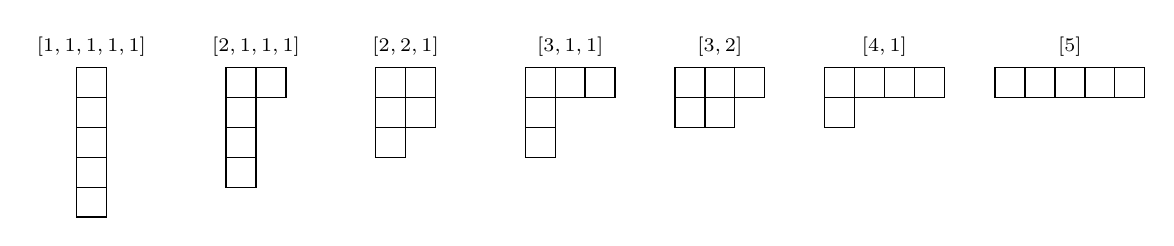
\begin{tikzpicture}[scale=.38,line width=.5pt]
\begin{scope}[shift={(0,0)}]
\draw (0,0) rectangle (1,-1);
\draw (0,-1) rectangle (1,-2);
\draw (0,-2) rectangle (1,-3);
\draw (0,-3) rectangle (1,-4);
\draw (0,-4) rectangle (1,-5);
\node[font=\scriptsize] at (0.5,.7) {$[1,1,1,1,1]$};
\end{scope}
\begin{scope}[shift={(5,0)}]
\draw (0,0) rectangle (1,-1);
\draw (1,0) rectangle (2,-1);
\draw (0,-1) rectangle (1,-2);
\draw (0,-2) rectangle (1,-3);
\draw (0,-3) rectangle (1,-4);
\node[font=\scriptsize] at (1.0,.7) {$[2,1,1,1]$};
\end{scope}
\begin{scope}[shift={(10,0)}]
\draw (0,0) rectangle (1,-1);
\draw (1,0) rectangle (2,-1);
\draw (0,-1) rectangle (1,-2);
\draw (1,-1) rectangle (2,-2);
\draw (0,-2) rectangle (1,-3);
\node[font=\scriptsize] at (1.0,.7) {$[2,2,1]$};
\end{scope}
\begin{scope}[shift={(15,0)}]
\draw (0,0) rectangle (1,-1);
\draw (1,0) rectangle (2,-1);
\draw (2,0) rectangle (3,-1);
\draw (0,-1) rectangle (1,-2);
\draw (0,-2) rectangle (1,-3);
\node[font=\scriptsize] at (1.5,.7) {$[3,1,1]$};
\end{scope}
\begin{scope}[shift={(20,0)}]
\draw (0,0) rectangle (1,-1);
\draw (1,0) rectangle (2,-1);
\draw (2,0) rectangle (3,-1);
\draw (0,-1) rectangle (1,-2);
\draw (1,-1) rectangle (2,-2);
\node[font=\scriptsize] at (1.5,.7) {$[3,2]$};
\end{scope}
\begin{scope}[shift={(25,0)}]
\draw (0,0) rectangle (1,-1);
\draw (1,0) rectangle (2,-1);
\draw (2,0) rectangle (3,-1);
\draw (3,0) rectangle (4,-1);
\draw (0,-1) rectangle (1,-2);
\node[font=\scriptsize] at (2.0,.7) {$[4,1]$};
\end{scope}
\begin{scope}[shift={(30.7,0)}]
\draw (0,0) rectangle (1,-1);
\draw (1,0) rectangle (2,-1);
\draw (2,0) rectangle (3,-1);
\draw (3,0) rectangle (4,-1);
\draw (4,0) rectangle (5,-1);
\node[font=\scriptsize] at (2.5,.7) {$[5]$};
\end{scope}
\end{tikzpicture}
\end{center}

\begin{definition}
\label{def:type}
$\sigma \in S_n$ 的\emph{型}%
\index{xing@型(type)}
是 $\langle\sigma\rangle$ 在 $\{\mathbf{1},\dots,\mathbf{n}\}$ 上作用的轨道大小给出的 $n$ 的划分.
\end{definition}

(由证明引理~\ref{lem:cycle-decomposition} 的论证) 希望已经清楚: $\sigma \in S_n$ 的型不过是由 $\sigma$ 作为不相交轮换之积的分解中各个轮换的长度, 再加上足够多的 $1$ 给出. 在我们的运行示例中,
\[
\sigma = (1\,8\,6\,3\,2)(4\,7) \in S_8
\]
有型 $[5,2,1]$:
\begin{center}
\ydiag{1/5,2/2,3/1}
\end{center}

引入``型''的主要原因, 是如下简单观察的推论.

\begin{lemma}
\label{lem:conjugate-cycle}
设 $\tau \in S_n$, 且 $(a_1 \dots a_r)$ 是一个轮换. 则
\[
\tau(a_1 \dots a_r)\tau^{-1} = (a_1\tau^{-1} \dots a_r\tau^{-1}).
\]
\end{lemma}

古怪的记号 $a_1\tau^{-1}$ 表示置换 $\tau^{-1}$ 在 $a_1 \in \{\mathbf{1},\dots,\mathbf{n}\}$ 上的作用; 回顾我们曾在 \S II.\ref{subsec:symmetric-groups} 约定让置换在右边作用, 以与群中乘积的惯用记号保持一致%
\footnote{别忘了置换在右边作用.}%
.

\begin{proof}
这通过验证两边在 $\{1,\dots,n\}$ 上作用相同来证明. 例如, 对 $1 \leq i < r$,
\[
(a_i\tau^{-1})(\tau(a_1 \dots a_r)\tau^{-1}) = a_i(a_1 \dots a_r)\tau^{-1} = a_{i+1}\tau^{-1}
\]
正如所应有; 其余情形留给读者.
\end{proof}

通过巧妙插入恒等因子 $\tau^{-1}\tau$ 的惯用手法, 这个计算共轭的公式立刻推广到任意轮换之积:
\[
\tau(a_1 \dots a_r)\dots(b_1 \dots b_s)\tau^{-1} = (a_1\tau^{-1} \dots a_r\tau^{-1})\dots(b_1\tau^{-1} \dots b_s\tau^{-1}).
\]
无论轮换是否不相交都成立. 然而, 由于 $\tau$ 是双射, 不相交的轮换在共轭后仍不相交. 这本质上就是如下重要观察的全部内容:

\begin{proposition}
\label{prop:conjugate-same-type}
$S_n$ 中两个元素在 $S_n$ 中共轭, 当且仅当它们有相同的型.
\end{proposition}

\begin{proof}
这个结论的``仅当''部分由上方的考虑立即得到: 共轭一个置换得到同型的置换. 至于``若''部分, 设
\[
\sigma_1 = (a_1 \dots a_r)(b_1 \dots b_s)\dots(c_1 \dots c_t)
\]
与
\[
\sigma_2 = (a_1' \dots a_r')(b_1' \dots b_s')\dots(c_1' \dots c_t')
\]
是两个同型的置换, 以轮换记号写出, 且 $r \geq s \geq \dots \geq t$ (于是型为 $[r,s,\dots,t]$). 令 $\tau$ 为任一满足 $a_i = a_i'\tau$, $b_j = b_j'\tau$, $\dots$, $c_k = c_k'\tau$ (对所有 $i,j,\dots,k$) 的置换. 则由引理~\ref{lem:conjugate-cycle} 有 $\sigma_2 = \tau\sigma_1\tau^{-1}$, 从而 $\sigma_1$ 与 $\sigma_2$ 共轭, 证毕.
\end{proof}

\begin{example}
\label{ex:conjugate-same-type}
在 $S_8$ 中,
\[
(1\,8\,6\,3\,2)(4\,7)\quad\text{与}\quad (1\,2\,3\,4\,5)(6\,7)
\]
必共轭, 因为它们同型. 命题~\ref{prop:conjugate-same-type} 的证明告诉我们
\[
\tau(1\,8\,6\,3\,2)(4\,7)\tau^{-1} = (1\,2\,3\,4\,5)(6\,7)
\]
对
\[
\tau = \begin{pmatrix} 1 & 2 & 3 & 4 & 5 & 6 & 7 & 8 \\ 1 & 8 & 6 & 3 & 2 & 4 & 7 & 5 \end{pmatrix}
\]
成立, 而当然这可以一秒钟内手算验证. 做这个验证, 特别是盯着 $\tau$ 的第二行相对于第一个置换的轮换记号看, 应当能澄清一切.
\end{example}

概括地说, 型 (或相应的 Young 图) 告诉我们关于 $S_n$ 中共轭的一切.

\begin{corollary}
\label{cor:conjugacy-classes-sn}
$S_n$ 中共轭类的个数等于 $n$ 的划分的个数.
\end{corollary}

例如, $S_5$ 中有 $7$ 个共轭类, 由上方画出的那些``像俄罗斯方块''的图所索引.

计算 $S_n$ 中每个共轭类的大小 (用型表示) 也相当直接. 例如, 为了数出 $S_5$ 中型 $[2,2,1]$ 的置换个数, 注意有 $5! = 120$ 种方式把数字 $1,\dots,5$ 填入相应的 Young 图:
\begin{center}
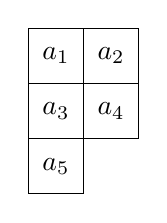
\begin{tikzpicture}[scale=.7,line width=.5pt]
\draw (0,0) rectangle (1,-1);
\node at (0.5,-0.5) {$a_1$};
\draw (1,0) rectangle (2,-1);
\node at (1.5,-0.5) {$a_2$};
\draw (0,-1) rectangle (1,-2);
\node at (0.5,-1.5) {$a_3$};
\draw (1,-1) rectangle (2,-2);
\node at (1.5,-1.5) {$a_4$};
\draw (0,-2) rectangle (1,-3);
\node at (0.5,-2.5) {$a_5$};
\end{tikzpicture}
\end{center}
也就是说, 有 $120$ 种方式把置换写成两个 $2$-轮换之积:
\[
(a_1 a_2)(a_3 a_4);
\]
但交换 $a_1 \leftrightarrow a_2$ 与 $a_3 \leftrightarrow a_4$, 以及交换两个轮换, 都给出同一个置换. 因此型 $[2,2,1]$ 的置换有
\[
\frac{120}{2 \cdot 2 \cdot 2} = 15
\]
个. 对 $S_5$ 的所有 Young 图做这个计算, 就得到每个共轭类的大小, 即 $S_5$ 的类公式 (参见 \S\ref{subsec:center-conjugacy}):
\[
120 = 1 + 10 + 15 + 20 + 20 + 30 + 24.
\]

\begin{example}
\label{ex:no-normal-30-s5}
$S_5$ 中没有大小为 $30$ 的正规子群.

的确, 正规子群是共轭类之并 (\S\ref{subsec:class-formula}); 由于单位元在每个子群中, 而 $30 - 1 = 29$ 不能写成 $S_5$ 的类公式中出现的那些数之和, 故不存在这样的子群.
\end{example}

这一观察将被我们即将证明的强得多的结果 (如定理~\ref{thm:an-simple}, 推论~\ref{cor:sn-not-solvable}) 所淹没; 但仅凭如此少的工作就能确立如此精确的陈述, 着实了不起.

\index{jiaocuoqun@交错群(alternating group)!you 3-lunhuanshengcheng@由 3-轮换生成(generated by 3-cycles)}\index{jiaocuoqun@交错群(alternating group)!zhongdegonge@中的共轭(conjugacy in)}\index{jiaocuoqun@交错群(alternating group)!A_n 对 n≥5 单@$A_n$ dui $n\ge 5$ dan}\subsection{对换、奇偶性与交错群}
\label{subsec:transpositions}

对 $n \geq 1$, 考虑多项式
\[
\Delta_n = \prod_{1 \leq i < j \leq n} (x_i - x_j) \in \Z[x_1,\dots,x_n],
\]
即
\[
\begin{aligned}
&\Delta_1 = 1,\\
&\Delta_2 = x_1 - x_2,\\
&\Delta_3 = (x_1 - x_2)(x_1 - x_3)(x_2 - x_3),\\
&\Delta_4 = (x_1 - x_2)(x_1 - x_3)(x_1 - x_4)(x_2 - x_3)(x_2 - x_4)(x_3 - x_4),
\end{aligned}
\]
我们可以让任意 $\sigma \in S_n$ 通过依 $\sigma$ 置换指标来作用于 $\Delta_n$:
\[
\Delta_n\sigma := \prod_{1 \leq i < j \leq n} (x_{i\sigma} - x_{j\sigma}).
\]
例如,
\[
\Delta_4(1\,2\,3\,4) = (x_2 - x_3)(x_2 - x_4)(x_2 - x_1)(x_3 - x_4)(x_3 - x_1)(x_4 - x_1) = -\Delta_4.
\]
一般地, 显然 $\Delta_n\sigma$ 仍是所有二项式 $(x_i - x_j)$ 之积, 只是因子被置换, 且某些因子可能在过程中变号. 因此 $\Delta_n\sigma = \pm\Delta_n$, 其中因子 $\pm 1$ 依赖于 $\sigma$.

\begin{definition}
\label{def:sign}
置换 $\sigma \in S_n$ 的\emph{符号}%
\index{fuhao@符号(symbol)}
由 $\sigma$ 对 $\Delta_n$ 的作用决定:
\[
\Delta_n\sigma = (-1)^\sigma \Delta_n.
\]
我们说一个置换是\emph{偶}%
\index{ouqizhihuan@偶/奇置换(even/odd permutation)}%
的, 如果它的符号是 $+1$; 是\emph{奇}的, 如果它的符号是 $-1$.
\end{definition}

注意对所有 $\sigma, \tau \in S_n$ 有
\[
\Delta_n(\sigma\tau) = (\Delta_n\sigma)\tau:
\]
由此得到 $(-1)^{\sigma\tau} = (-1)^\sigma(-1)^\tau$. 把 $\{-1,+1\}$ 视为乘法群%
\footnote{这是 $\Z$ 的单位群; 当然它同构于 $C_2$.}%
, 我们看到``符号''函数
\[
\epsilon : S_n \to \{-1,+1\},\quad \epsilon(\sigma) := (-1)^\sigma
\]
是一个同态.

看待这个符号函数的另一个视角如下. 一个\emph{对换}%
\index{duihuan@对换(transposition)}
是长度为 $2$ 的轮换. 每个置换都是对换之积:

\begin{lemma}
\label{lem:transpositions-generate}
对换生成 $S_n$.
\end{lemma}

\begin{proof}
的确, 由引理~\ref{lem:cycle-decomposition} 只需证明每个轮换都是对换之积, 而
\[
(a_1 \dots a_r) = (a_1 a_2)(a_1 a_3)\dots(a_1 a_r),
\]
这可通过把两边作用于 $\{1,\dots,n\}$ 的每个元素来验证.
\end{proof}

当然, 一个给定的置换可以写成对换之积的方式有很多种. 然而, 究竟需要偶数个还是奇数个对换, 只依赖于 $\sigma$. 的确,

\begin{lemma}
\label{lem:transposition-parity}
设 $\sigma = \tau_1 \dots \tau_r$ 是对换之积. 则 $\sigma$ 是偶的, 相应地, 奇的, 按照 $r$ 是偶的, 相应地, 奇的.
\end{lemma}

\begin{proof}
这由 $\epsilon$ 是同态、以及对换的符号为 $-1$ 立即得到: 的确, $(ij)$ 作用于 $\Delta_n$ 时置换其因子并改变奇数个因子的符号: 即 $(x_i-x_j)$, 以及每个 $i<k<j$ 所对应的两个因子 $(x_i-x_k)$ 和 $(x_k-x_j)$.
\end{proof}

\begin{definition}
\label{def:alternating}
$\{\mathbf{1},\dots,\mathbf{n}\}$ 上的\emph{交错群}%
\index{jiaocuoqun@交错群(alternating group)}
, 记作 $A_n$, 由 $S_n$ 中所有偶置换组成.
\end{definition}

交错群是 $S_n$ 的正规子群, 且对 $n \geq 2$ 有
\[
[S_n : A_n] = 2:
\]
的确, $A_n = \Ker \epsilon$, 且对 $n \geq 2$ 有 $\epsilon$ 满.

依据 $\sigma$ 的型来判断 $\sigma$ 是否属于 $A_n$ 非常容易. 的确 (由证明引理~\ref{lem:transpositions-generate} 的论证), 一个轮换是偶的, 相应地, 奇的, 若它的长度是奇的, 相应地, 偶的%
\footnote{注意这不幸的术语冲突. 例如, $3$-轮换是偶置换.}%
. 形象地说, $\sigma \in S_n$ 是偶的, 当且仅当 $n$ 与 $\sigma$ 的 Young 图的行数有相同的奇偶性. 以 $n = 5$ 为例, 七个型中偶者加星标:
\begin{center}
\begin{tikzpicture}[scale=.38,line width=.5pt]
\begin{scope}[shift={(0,0)}]
\draw (0,0) rectangle (1,-1);
\draw (0,-1) rectangle (1,-2);
\draw (0,-2) rectangle (1,-3);
\draw (0,-3) rectangle (1,-4);
\draw (0,-4) rectangle (1,-5);
\node at (0.5,.7) {$\star$};
\end{scope}
\begin{scope}[shift={(2.7,0)}]
\draw (0,0) rectangle (1,-1);
\draw (1,0) rectangle (2,-1);
\draw (0,-1) rectangle (1,-2);
\draw (0,-2) rectangle (1,-3);
\draw (0,-3) rectangle (1,-4);
\end{scope}
\begin{scope}[shift={(6.4,0)}]
\draw (0,0) rectangle (1,-1);
\draw (1,0) rectangle (2,-1);
\draw (0,-1) rectangle (1,-2);
\draw (1,-1) rectangle (2,-2);
\draw (0,-2) rectangle (1,-3);
\node at (1.0,.7) {$\star$};
\end{scope}
\begin{scope}[shift={(10.100000000000001,0)}]
\draw (0,0) rectangle (1,-1);
\draw (1,0) rectangle (2,-1);
\draw (2,0) rectangle (3,-1);
\draw (0,-1) rectangle (1,-2);
\draw (0,-2) rectangle (1,-3);
\node at (1.5,.7) {$\star$};
\end{scope}
\begin{scope}[shift={(14.8,0)}]
\draw (0,0) rectangle (1,-1);
\draw (1,0) rectangle (2,-1);
\draw (2,0) rectangle (3,-1);
\draw (0,-1) rectangle (1,-2);
\draw (1,-1) rectangle (2,-2);
\end{scope}
\begin{scope}[shift={(19.5,0)}]
\draw (0,0) rectangle (1,-1);
\draw (1,0) rectangle (2,-1);
\draw (2,0) rectangle (3,-1);
\draw (3,0) rectangle (4,-1);
\draw (0,-1) rectangle (1,-2);
\end{scope}
\begin{scope}[shift={(25.2,0)}]
\draw (0,0) rectangle (1,-1);
\draw (1,0) rectangle (2,-1);
\draw (2,0) rectangle (3,-1);
\draw (3,0) rectangle (4,-1);
\draw (4,0) rectangle (5,-1);
\node at (2.5,.7) {$\star$};
\end{scope}
\end{tikzpicture}
\end{center}
加星标的型对应偶置换. 把这些型对应的共轭类大小相加,
\[
1 + 15 + 20 + 24 = 60,
\]
确认了 $A_5$ 在 $S_5$ 中指数为 $2$.

然而, 不要对这个计算过度解读: 我们并不是在断言这些就是 $A_5$ 中共轭类的大小, 而只是说这些是构成正规子群 $A_5$ 的、在 $S_5$ 中的共轭类. $A_n$ 中的共轭相当有趣, 并与 $A_n$ 的单性这一问题精巧地牵连在一起.

\subsection{\texorpdfstring{$A_n$}{An} 中的共轭; \texorpdfstring{$A_n$}{An} 的单性与 \texorpdfstring{$S_n$}{Sn} 的可解性}
\label{subsec:an-simplicity}

以 $[\sigma]_{S_n}$, 相应地, $[\sigma]_{A_n}$ 记偶置换 $\sigma$ 在 $S_n$, 相应地, $A_n$ 中的共轭类. 显然 $[\sigma]_{A_n} \subseteq [\sigma]_{S_n}$; 我们来比较这两个集合.

\begin{lemma}
\label{lem:an-conjugacy-size}
设 $n \geq 2$, $\sigma \in A_n$. 则 $[\sigma]_{A_n} = [\sigma]_{S_n}$, 或 $[\sigma]_{A_n}$ 的大小是 $[\sigma]_{S_n}$ 大小的一半, 按照中心化子 $Z_{S_n}(\sigma)$ 不含于, 还是含于 $A_n$.
\end{lemma}

\begin{proof}
(参见习题~\ref{ex:index-2-classes}.) 注意
\[
Z_{A_n}(\sigma) = A_n \cap Z_{S_n}(\sigma):
\]
这由中心化子的定义 (定义~\ref{def:centralizer}) 立即得到. 现在回忆 $\sigma$ 的中心化子是对 $\sigma$ 作共轭时的稳定子, 因此 $\sigma$ 的共轭类的大小等于其中心化子的指数.

若 $Z_{S_n}(\sigma) \subseteq A_n$, 则 $Z_{A_n}(\sigma) = Z_{S_n}(\sigma)$, 于是
\[
[S_n : Z_{S_n}(\sigma)] = [S_n : Z_{A_n}(\sigma)] = [S_n : A_n][A_n : Z_{A_n}(\sigma)] = 2 \cdot [A_n : Z_{A_n}(\sigma)];
\]
因此在此情形下 $[\sigma]_{A_n}$ 是 $[\sigma]_{S_n}$ 大小的一半.

若 $Z_{S_n}(\sigma) \not\subseteq A_n$, 则注意 $A_n Z_{S_n}(\sigma) = S_n$: 的确, $A_n Z_{S_n}(\sigma)$ 是 $S_n$ 的子群 (因为 $A_n$ 正规; 参见命题~II.\ref{prop:second-iso}), 且真包含 $A_n$, 因此由于 $A_n$ 在 $S_n$ 中指数为 $2$, 它必等于 $S_n$. 应用第二同构定理 (命题~II.\ref{prop:second-iso}) 得到
\[
[A_n : Z_{A_n}(\sigma)] = [A_n : A_n \cap Z_{S_n}(\sigma)] = [A_n Z_{S_n}(\sigma) : Z_{S_n}(\sigma)] = [S_n : Z_{S_n}(\sigma)],
\]
因此这两个类大小相同. 既然在任何情形下都有 $[\sigma]_{A_n} \subseteq [\sigma]_{S_n}$, 便推出 $[\sigma]_{A_n} = [\sigma]_{S_n}$, 证毕.
\end{proof}

于是, 偶置换的共轭类或者从 $S_n$ 保持到 $A_n$, 或者分裂成两个不同的、等大小的类. 我们现在可以给出精确判定何时发生分裂的条件.

\begin{proposition}
\label{prop:an-split}
设 $\sigma \in A_n$, $n \geq 2$. 则 $\sigma$ 在 $S_n$ 中的共轭类在 $A_n$ 中分裂成两个共轭类, 当且仅当 $\sigma$ 的型由互不相同的奇数组成.
\end{proposition}

\begin{proof}
由引理~\ref{lem:an-conjugacy-size}, 我们须验证: $Z_{S_n}(\sigma)$ 含于 $A_n$, 当且仅当所述条件满足; 也就是说, 我们须证明
\[
\sigma = \tau\sigma\tau^{-1} \implies \tau\text{ 是偶的}
\]
当且仅当 $\sigma$ 的型由互不相同的奇数组成.

把 $\sigma$ 写成轮换记号 (包括长度为 $1$ 的轮换):
\[
\sigma = (a_1 \dots a_\lambda)(b_1 \dots b_\mu)\dots(c_1 \dots c_\nu),
\]
并回顾 (引理~\ref{lem:conjugate-cycle}) 有
\[
\tau\sigma\tau^{-1} = (a_1\tau^{-1} \dots a_\lambda\tau^{-1})(b_1\tau^{-1} \dots b_\mu\tau^{-1})\dots(c_1\tau^{-1} \dots c_\nu\tau^{-1}).
\]
假设 $\lambda,\mu,\dots,\nu$ 都是奇数且互不相同. 若 $\tau\sigma\tau^{-1} = \sigma$, 则由于所有轮换长度不同, $\tau$ 的共轭必须保持 $\sigma$ 的每个轮换:
\[
\tau(a_1 \dots a_\lambda)\tau^{-1} = (a_1 \dots a_\lambda),\quad\text{等等},
\]
也就是说,
\[
(a_1\tau^{-1} \dots a_\lambda\tau^{-1}) = (a_1 \dots a_\lambda),\quad\text{等等}.
\]
这意味着 $\tau$ 在 (例如) $a_1,\dots,a_\lambda$ 上作为一个循环置换作用, 因此其作用与 $(a_1 \dots a_\lambda)$ 的一个幂相同. 由此推出
\[
\tau = (a_1 \dots a_\lambda)^r(b_1 \dots b_\mu)^s\dots(c_1 \dots c_\nu)^t
\]
对适当的 $r,s,\dots,t$ 成立. 由于所有轮换长度都是奇数, 每个轮换都是偶置换; 而 $\tau$ 作为偶置换之积也必是偶的. 这就证明了: 若所述条件成立, 则 $Z_{S_n}(\sigma) \subseteq A_n$.

反之, 假设所述条件不成立: 也就是说, $\sigma$ 的轮换分解中要么有某个轮换长度为偶数, 要么所有轮换长度都是奇数但其中两个长度相同.

在第一种情形下, 令 $\tau$ 是 $\sigma$ 的轮换分解中一个偶长度的轮换. 注意 $\tau\sigma\tau^{-1} = \sigma$: 的确, $\tau$ 与自身交换, 也与 $\sigma$ 中除 $\tau$ 外的所有轮换交换. 由于 $\tau$ 长度为偶, 它作为置换是奇的: 这表明 $Z_{S_n}(\sigma) \not\subseteq A_n$, 证毕.

在第二种情形下, 不妨设 $\lambda = \mu$, 并考虑奇置换
\[
\tau = (a_1 b_1)(a_2 b_2)\dots(a_\lambda b_\lambda):
\]
用 $\tau$ 作共轭只是交换了 $\sigma$ 的前两个轮换; 因此 $\tau\sigma\tau^{-1} = \sigma$. 由于 $\tau$ 是奇的, 这再次表明 $Z_{S_n}(\sigma) \not\subseteq A_n$, 证毕.
\end{proof}

\begin{example}
\label{ex:a5-conjugacy}
再看 $A_5$, 我们在 \S\ref{subsec:transpositions} 中已注意到 $S_5$ 中偶置换的型是 $[1,1,1,1,1]$, $[2,2,1]$, $[3,1,1]$ 与 $[5]$. 由命题~\ref{prop:an-split}, 前三种型对应的共轭类在 $A_5$ 中保持不变, 而最后一种分裂.

因此 $A_5$ 恰好有 $5$ 个共轭类, 且 $A_5$ 的类公式是
\[
60 = 1 + 15 + 20 + 12 + 12.
\]
\end{example}

终于! 我们现在可以补全本章第一节开启的思路之环. 一路上, 读者应当已经验证了每个阶 $< 60$ 的单群都是交换的 (习题~\ref{ex:no-simple-below-60}); 而我们现在看到了 $60$ 为何特殊:

\begin{corollary}
\label{cor:a5-simple}
交错群 $A_5$ 是一个 $60$ 阶的非交换单群.
\end{corollary}

\begin{proof}
$A_5$ 的正规子群必是共轭类之并, 包含单位元, 且阶等于 $60$ 的一个因子 (由 Lagrange 定理). $60$ 的除 $1$ 与 $60$ 外的因子是
\[
2, 3, 4, 5, 6, 10, 12, 15, 20, 30;
\]
除单位元外计数的元素个数将是类公式中若干 $\neq 1$ 的数之和, 即下列之一:
\[
1, 2, 3, 4, 5, 9, 11, 14, 19, 29.
\]
\index{gen@根(radical)!duoxiangshide@多项式的(of a polynomial)}但这根本不会发生.
\end{proof}

读者将用同样的方法验证 $A_6$ 是单的 (习题~\ref{ex:a6-simple}). 事实上, 所有群 $A_n$ ($n \geq 5$) 都是单的 (且非交换), 这蕴含对 $n \geq 5$ 有 $S_n$ 不可解; 鉴于其在 Galois 理论中的应用 (例如推论~VII.\ref{cor:galois-criterion}), 这些事实相当重要. 注意 $A_2$ 平凡, $A_3 \cong \Z/3\Z$ 是单且交换的, 而 $A_4$ 不是单的 (习题~\ref{ex:no-simple-below-60})%
\footnote{好做法是先从较小的例子入手: 例如, 正四面体旋转群同构于 $A_4$.}%
.

\index{ershimiantiqun@二十面体群(icosahedral group)}交错群 $A_5$ 也称为\emph{二十面体} (旋转) 群: 的确, 它是通过刚体运动得到的一个二十面体的对称群. (读者能验证这一事实吗?)

$A_n$ 对 $n \geq 5$ 的单性可以通过研究 $3$-轮换来建立. 首先自然会问: 是否每个偶置换都可写成 $3$-轮换之积? 答案的确是肯定的:

\begin{lemma}
\label{lem:an-3cycles}
交错群 $A_n$ 由 $3$-轮换生成.
\end{lemma}

\begin{proof}
由于每个偶置换都是偶数个 $2$-轮换之积, 只需证明每两个 $2$-轮换之积都可写成 $3$-轮换之积. 因此考虑乘积
\[
(ab)(cd)
\]
其中 $a \neq b$, $c \neq d$. 若 $(ab) = (cd)$, 则这个乘积是单位元, 无可证. 若 $\{a,b\}$, $\{c,d\}$ 恰有一个公共元素, 则可设 $c = a$, 并观察到
\[
(ab)(ad) = (a\, b\, d).
\]
若 $\{a,b\}$, $\{c,d\}$ 不相交, 则
\[
(ab)(cd) = (a\, b\, c)(a\, d\, c),
\]
证毕.
\end{proof}

现在我们可利用对 $A_n$ 中共轭的研究:

\begin{claim}
\label{claim:an-normal-3cycle}
设 $n \geq 5$. 若 $A_n$ 的一个正规子群包含一个 $3$-轮换, 则它包含所有 $3$-轮换.
\end{claim}

\begin{proof}
正规子群是共轭类之并, 因此我们只需验证: 对 $n \geq 5$, $3$-轮换在 $A_n$ 中构成一个共轭类. 但它们在 $S_n$ 中确实如此, 且一个 $3$-轮换的型对 $n \geq 5$ 是 $[3,1,1,\dots]$; 因此由命题~\ref{prop:an-split}, 该共轭类在 $A_n$ 中不分裂.
\end{proof}

一般的陈述现在通过收尾而轻易得到:

\begin{theorem}
\label{thm:an-simple}
对 $n \geq 5$, 交错群 $A_n$ 是单的.
\end{theorem}

\begin{proof}
对 $n = 5$ 我们已经验证; 读者对 $n = 6$ 也已验证. 对 $n > 6$, 设 $N$ 是 $A_n$ 的非平凡正规子群; 我们将通过证明 $N$ 包含 $3$-轮换来表明必有 $N = A_n$.

令 $\tau \in N$, $\tau \neq (1)$, 并设 $\sigma \in A_n$ 是一个 $3$-轮换. 由于 $A_n$ 的中心平凡 (习题~\ref{ex:center-an}) 且 $3$-轮换生成 $A_n$, 我们可设 $\tau$ 与 $\sigma$ 不交换, 即换位子
\[
[\tau,\sigma] = \tau(\sigma\tau^{-1}\sigma^{-1}) = (\tau\sigma\tau^{-1})\sigma^{-1}
\]
不是单位元. 这个元素在 $N$ 中 (由第一个表达式显见, 因 $N$ 正规), 且是两个 $3$-轮换之积 (由第二个表达式显见, 因为 $3$-轮换的共轭仍是 $3$-轮换).

因此, 必要时用 $[\tau,\sigma]$ 替换 $\tau$, 我们可设 $\tau \in N$ 是一个作用在 $\leq 6$ 个元素上的非单位置换: 也就是说, 作用在 $\{1,\dots,n\}$ 的某个子集 $T$ 上, 且 $|T| = 6$. 现在我们可以通过让 $A_6$ 作用在 $T$ 上, 把 $A_6$ 视为 $A_n$ 的子群. 于是 $A_6$ 的子群 $N \cap A_6$ 是正规的 (因 $N$ 正规) 且非平凡 (因 $\tau \in N \cap A_6$ 且 $\tau \neq (1)$). 由于 $A_6$ 单 (习题~\ref{ex:a6-simple}), 这蕴含 $N \cap A_6 = A_6$. 特别地, $N$ 包含 $3$-轮换.

由断言~\ref{claim:an-normal-3cycle}, 这蕴含 $N$ 包含所有 $3$-轮换. 再由引理~\ref{lem:an-3cycles} 推出 $N = A_n$, 证毕.
\end{proof}

\begin{corollary}
\label{cor:sn-not-solvable}
对 $n \geq 5$, 群 $S_n$ 不可解.
\end{corollary}

\begin{proof}
由于 $A_n$ 单, 序列
\[
S_n \supsetneqq A_n \supsetneqq \{(1)\}
\]
是 $S_n$ 的一个合成列. 由此推出 $S_n$ 的合成因子是 $\Z/2\Z$ 与 $A_n$. 由命题~\ref{prop:solvable-equiv}, $S_n$ 不可解.
\end{proof}

特别地, $S_5$ 是一个 $120$ 阶的非可解群. 这事实上是非单且不可解群的最小阶; 参见习题~\ref{ex:order-less-120-solvable}.

\subsection*{习题}
\phantomsection
\addcontentsline{toc}{subsection}{习题}

\begin{prob}
\label{ex:conj-class-size}
$\triangleright$ 计算 $S_8$ 中
\[
\begin{pmatrix} 1 & 2 & 3 & 4 & 5 & 6 & 7 & 8 \\ 8 & 1 & 2 & 7 & 5 & 3 & 4 & 6 \end{pmatrix}
\]
的共轭类中的元素个数. [§\ref{subsec:cycle-notation}]
\end{prob}

\begin{prob}
\label{ex:cycle-unique}
$\triangleright$ 设
\[
(a_1 \dots a_r)(b_1 \dots b_s)\dots(c_1 \dots c_t) = (d_1 \dots d_u)(e_1 \dots e_v)\dots(f_1 \dots f_w)
\]
\index{ji@积(product)!mode@模的(of a module)}是两个不相交轮换之积. 证明这些因子可差次序而一致.

(提示: 这两个对应的 $\{\mathbf{1},\dots,\mathbf{n}\}$ 的划分必须一致.) [§\ref{subsec:cycle-notation}]
\end{prob}

\begin{prob}
\label{ex:cycle-order}
设 $\sigma$ 有型 $[\lambda_1,\dots,\lambda_r]$, 且诸 $\lambda_i$ 两两互素. $|\sigma|$ 是什么? 去掉关于这些数的额外假设, 你能对 $|\sigma|$ 说什么?
\end{prob}

\begin{prob}
\label{ex:partition-generating}
弄懂无穷乘积
\[
\frac{1}{1 - x} \cdot \frac{1}{1 - x^2} \cdot \frac{1}{1 - x^3} \cdot \frac{1}{1 - x^4} \cdot \frac{1}{1 - x^5} \cdot \dots
\]
的``Taylor 级数''. 证明该级数中 $x^n$ 的系数就是 $n$ 的划分的个数.
\end{prob}

\begin{prob}
\label{ex:class-formula-small}
求 $S_n$ ($n \leq 6$) 的类公式.
\end{prob}

\begin{prob}
\label{ex:s4-normal-size}
设 $N$ 是 $S_4$ 的正规子群. 证明 $|N| = 1, 4, 12$ 或 $24$.
\end{prob}

\begin{prob}
\label{ex:sn-generated}
$\triangleright$ 证明 $S_n$ 由 $(12)$ 与 $(12\dots n)$ 生成.

(提示: 只要得到所有对换即可. $(12\dots n)$ 对 $(12)$ 的共轭是什么?) [\ref{ex:s4-generated-d8}, §VII.\ref{subsec:poly-galois-groups}]
\end{prob}

\begin{prob}
\label{ex:s4-dihedral}
$\neg$ 对 $n > 1$, 证明由固定 $\mathbf{1}$ 的置换组成的 $S_n$ 的子群 $H$ 同构于 $S_{n-1}$. 证明不存在真包含 $H$ 的 $S_n$ 的真子群. [VII.\ref{ex:sn-galois-sn-1}]
\end{prob}

\begin{prob}
\label{ex:s4-generated-d8}
由习题~\ref{ex:sn-generated}, $S_4$ 由 $(12)$ 与 $(1234)$ 生成. 证明 $(13)$ 与 $(1234)$ 在 $S_4$ 中生成一个 $D_8$ 的拷贝. 证明 $S_4$ 的每个 $8$ 阶子群都共轭于 $\langle (13), (1234) \rangle$. 证明恰有 $3$ 个这样的子群. 对所有 $n \geq 3$ 证明 $S_n$ 包含一个二面体群 $D_{2n}$ 的拷贝, 并找出其生成元.
\end{prob}

\begin{prob}
\label{ex:n-cycles-count}
$\neg$ $\bullet$ 证明 $S_n$ 中恰有 $(n - 1)!$ 个 $n$-轮换.

$\bullet$ 更一般地, 求 $S_n$ 中给定型的置换的共轭类大小公式. [\ref{ex:sylow-sp}]
\end{prob}

\begin{prob}
\label{ex:sylow-sp}
设 $p$ 是素整数. 计算 $S_p$ 的 $p$-Sylow 子群的个数. (使用习题~\ref{ex:n-cycles-count}.) 用这个结果与第三西罗定理再次证明 Wilson 定理的``仅当''方向 (参见习题~II.\ref{ex:wilson}).
\end{prob}

\begin{prob}
\label{ex:transitive-subgroups}
$\triangleright$ 子群 $G \subseteq S_n$ 是\emph{传递的}, 如果 $G$ 在 $\{1,\dots,n\}$ 上的诱导作用是传递的.
\begin{itemize}
\item 证明若 $G \subseteq S_n$ 传递, 则 $|G|$ 是 $n$ 的倍数.
\item 列出 $S_3$ 的传递子群.
\item 证明如下 $S_4$ 的子群都是传递的:
\begin{itemize}
\item $\langle (1234) \rangle \cong C_4$ 及其共轭,
\item $\langle (1\,2)(3\,4), (1\,3)(2\,4) \rangle \cong C_2 \times C_2$,
\item $\langle (1\,2)(3\,4), (1\,2\,3\,4) \rangle \cong D_8$ 及其共轭,
\item $A_4$, 以及 $S_4$.
\end{itemize}
\end{itemize}
稍费些耐力, 你可以证明这些就是 $S_4$ 仅有的传递子群.

[§VII.\ref{subsec:poly-galois-groups}]
\end{prob}

\begin{prob}
\label{ex:sign-determinant}
(若你了解行列式.) 证明定义~\ref{def:sign} 中置换 $\sigma$ 的符号等于习题~II.\ref{ex:permutation-matrix} 中定义的矩阵 $M_\sigma$ 的行列式.
\end{prob}

\begin{prob}
\label{ex:center-an}
$\triangleright$ 证明对 $n \geq 4$, $A_n$ 的中心平凡. [§\ref{subsec:an-simplicity}]
\end{prob}

\begin{prob}
\label{ex:even-pictorial}
证实施加于 \S\ref{subsec:transpositions} 的、判断一个置换是否偶的``形象''法则.
\end{prob}

\begin{prob}
\label{ex:an-conj-classes-list}
$n \geq 2$ 时 $A_n$ 中共轭类的个数 (据称) 为
\[
1, 3, 4, 5, 7, 9, 14, 18, 24, 31, 43, \dots
\]
通过求出相应交错群的类公式, 核对这个表中的前几项.
\end{prob}

\begin{prob}
\label{ex:a4-class-formula}
$\triangleright$ $\bullet$ 求 $A_4$ 的类公式.

$\bullet$ 用它证明 $A_4$ 没有 $6$ 阶子群. [§II.\ref{subsec:index-lagrange}]
\end{prob}

\begin{prob}
\label{ex:an-index-n}
对 $n \geq 5$, 设 $H$ 是 $A_n$ 的真子群. 证明 $[A_n : H] \geq n$. 证明对所有 $n \geq 3$, $A_n$ 确实有一个指数为 $n$ 的子群.
\end{prob}

\begin{prob}
\label{ex:an-no-small-action}
设 $n\geq5$. 证明对 $|S| < n$ 的任意集合 $S$, $A_n$ 在 $S$ 上没有非平凡作用. 构造 $A_4$ 在集合 $S$ ($|S| = 3$) 上的一个非平凡作用\footnote{如果你愿意可以代数地思考; 如果你更喜欢几何, 可以想象正四面体的对棱\erratumfootnote{根据官方勘误, 原书英文此处将 sides 修正为 edges (棱).}.}. $A_4$ 在 $|S| = 2$ 的集合 $S$ 上是否有非平凡作用?
\end{prob}

\begin{prob}
\label{ex:a5-sylow-5}
$\neg$ 找出 $A_5$ 中所有十五个 $2$ 阶元素, 并证明 $A_5$ 恰有五个 $2$-Sylow 子群. [\ref{ex:unique-simple-60}]
\end{prob}

\begin{prob}
\label{ex:a6-simple}
$\triangleright$ 用其类公式 (如同在推论~\ref{cor:a5-simple} 的证明中对 $A_5$ 所做的那样) 证明 $A_6$ 是单的. [§\ref{subsec:an-simplicity}]
\end{prob}

\begin{prob}
\label{ex:unique-simple-60}
$\neg$ 验证 $A_5$ 是 (在同构意义下) 唯一的 $60$ 阶单群. (提示: 由习题~\ref{ex:simple-60}, 一个 $60$ 阶单群 $G$ 含有一个指数为 $5$ 的子群. 利用这一事实构造同态 $G \to S_5$, 并证明该同态的像必是 $A_5$.)\erratumfootnote{根据官方勘误, 明确解题提示.} 注意 $A_5$ 恰有五个 $2$-Sylow 子群; 参见习题~\ref{ex:a5-sylow-5}. 于是习题~\ref{ex:simple-60} 中考虑的另一个可能性不会出现. [\ref{ex:simple-60}]
\end{prob}

\section{群的积}
\label{sec:products-of-groups}

我们已经知道直积存在于 $\cate{Grp}$ 中 (参见 \S II.\ref{subsec:products-grp}); 这里我们进一步分析这一概念, 并探讨同一主题的一些变体, 着眼于这样一个问题: 要由合成因子重构一个群, 究竟需要哪些信息.

\subsection{直积}
\label{subsec:direct-product}

回顾 \S II.\ref{subsec:products-grp}: 两个群 $H$, $K$ 的 (直) 积是指支撑在集合 $H \times K$ 上, 运算按分量定义的群. 我们已验证过 (命题~II.\ref{prop:product-grp}): 直积满足在范畴 $\cate{Grp}$ 中定义积运算的泛性质.

存在这样的情形: 群 $G$ 的两个子群 $N$, $H$ 的直积可以实化为 $G$ 的一个子群. 回顾 (命题~II.\ref{prop:second-iso}): 若其中一个子群正规, 则 $G$ 的子集 $NH$ 事实上是 $G$ 的一个子群. $NH$ 与 $N \times H$ 之间的关系取决于 $N$ 与 $H$ 在 $G$ 中如何相交, 于是我们先来看看这个交集.

$G$ 的两个子集 $A$, $B$ 的\emph{换位子}%
\index{weihuanzi@换位子(commutator)}
$[A, B]$ (参见 \S\ref{subsec:commutator}) 是指所有形如 $[a, b]$ ($a \in A$, $b \in B$) 的换位子生成的子群.

\begin{lemma}
\label{lem:commutator-subset}
设 $N$, $H$ 是群 $G$ 的正规子群. 则
\[
[N, H] \subseteq N \cap H.
\]
\end{lemma}

\begin{proof}
只需在生成元上验证; 也就是说, 只需验证对所有 $n \in N$, $h \in H$ 都有
\[
[n, h] = n(h n^{-1} h^{-1}) = (n h n^{-1}) h^{-1} \in N \cap H.
\]
但第一个表达式与 $N$ 的正规性说明 $[n, h] \in N$; 第二个表达式与 $H$ 的正规性说明 $[n, h] \in H$.
\end{proof}

\begin{corollary}
\label{cor:normal-intersect-trivial}
设 $N$, $H$ 是群 $G$ 的正规子群. 假设 $N \cap H = \{e\}$. 则 $N$, $H$ 彼此交换:
\[
(\forall n \in N)\,(\forall h \in H) \quad n h = h n.
\]
\end{corollary}

\begin{proof}
由引理~\ref{lem:commutator-subset}, 若 $N \cap H = \{e\}$ 则 $[N, H] = \{e\}$; 结论立得.
\end{proof}

事实上, 在同一假设下还能得到更多:

\begin{proposition}
\label{prop:normal-intersection-direct}
设 $N$, $H$ 是群 $G$ 的正规子群, 且满足 $N \cap H = \{e\}$. 则 $NH \cong N \times H$.
\end{proposition}

\begin{proof}
考虑由 $\varphi(n, h) = nh$ 定义的函数
\[
\varphi : N \times H \to N H.
\]
在所给假设下, $\varphi$ 是一个群同态: 的确,
\[
\begin{array}{r}
\varphi((n_1, h_1) \cdot (n_2, h_2)) = \varphi((n_1 n_2, h_1 h_2)) \\
= n_1 n_2 h_1 h_2 \\
= n_1 h_1 n_2 h_2
\end{array}
\]
(因为由推论~\ref{cor:normal-intersect-trivial}, $N$, $H$ 交换)
\[
= \varphi((n_1, h_1)) \cdot \varphi((n_2, h_2)).
\]
同态 $\varphi$ 由 $NH$ 的定义显然是满的. 为验证它是单的, 考虑它的核:
\[
\ker \varphi = \{(n, h) \in N \times H \mid n h = e\}.
\]
若 $nh = e$, 则 $n \in N$ 且 $n = h^{-1} \in H$; 从而因 $N \cap H = \{e\}$ 有 $n = e$. 同理对 $h$ 可得 $h = e$; 于是 $(n, h)$ 是 $N \times H$ 中的单位元, 这就证明了 $\varphi$ 是单的.

因此 $\varphi$ 是同构, 证毕.
\end{proof}

\begin{remark}
\label{rem:pq-cyclic-alt}
这个结果给出了断言~2.16 证明的另一个论证: 若 $|G| = pq$, 其中 $p < q$ 为素数, 且 $G$ 含有阶分别为 $p$, $q$ 的正规子群 $H$, $K$ (当 $q \not\equiv 1 \bmod p$ 时由西罗定理即如此), 则必有 $H \cap K = \{e\}$, 于是命题~\ref{prop:normal-intersection-direct} 表明 $HK \cong H \times K$. 由于 $|HK| = |G| = pq$, 这就证明了 $G \cong H \times K \cong \mathbb{Z}/p\mathbb{Z} \times \mathbb{Z}/q\mathbb{Z}$. 最后, $(1, 1)$ 在这个群中的阶为 $pq$, 故 $G$ 是循环的, 从而我们得到了与断言~2.16 相同的结论.
\end{remark}

\subsection{群的正合列; 扩张问题}
\label{subsec:exact-sequences}

当然, 命题~\ref{prop:normal-intersection-direct} 的结论要求两个子群 $N$, $H$ 都正规: 例如, 置换 $(123)$ 与 $(12)$ 生成 $S_3$ 中仅交于 $\{e\}$ 的子群 $N$, $H$, 且 $N$ 在 $S_3$ 中正规, 但 $S_3 = NH$ 并不同构于 $N$ 与 $H$ 的直积. 考察这一更一般的情形是很自然的.

设 $N$, $H$ 是群 $G$ 的子群, $N$ 正规 (但对 $H$ 没有先验假设), 且满足 $N \cap H = \{e\}$; 并假设 $G = NH$. 我们意在用 $N$ 与 $H$ 的结构来描述 $G$ 的结构.

使用正合列%
\index{zhenghelie@正合列(exact sequence)}%
\index{kuozhang@扩张(extension)}
的语言较为方便, 这一语言我们在 \S III.\ref{subsec:complexes} 中为模引入过. 群的一个 (短) 正合列是指一列群与群同态
\[
1 \longrightarrow N \stackrel{\varphi}{\longrightarrow} G \stackrel{\psi}{\longrightarrow} H \longrightarrow 1,
\]
其中 $\psi$ 是满的, 且 $\varphi$ 把 $N$ 等同于 $\ker \psi$. 换言之 (由第一同构定理), 用 $\varphi$ 把 $N$ 等同于 $G$ 的一个子群; 那么该列正合当且仅当 $N$ 在 $G$ 中正规, 且 $\psi$ 诱导出同构 $G/N \cong H$.

读者不妨稍停片刻, 验证: 若 $G$, $N$, $H$ 都是交换群, 那么这个概念与 \S III.\ref{subsec:complexes} 中交换群 (即 $\mathbb{Z}$-模) 的短正合列的概念精确吻合; 一个记号上的差别是: 这里平凡群记作 `1' 而非 `0'%
\footnote{这并非没有道理, 因为群更常以``乘法''而非``加法''书写, 所以单位元更可能记作 $1$ 而非 $0$.}%
.

当然总存在一个正合列
\[
1 \longrightarrow N \longrightarrow N \times H \longrightarrow H \longrightarrow 1:
\]
把 $n \in N$ 映到 $(n, e_H)$, 把 $(n, h) \in N \times H$ 映到 $h$. 不过请记住这是一个非常特殊的情形: 重提上面提到的例子, 也存在正合列
\[
1 \longrightarrow C_3 \longrightarrow S_3 \longrightarrow C_2 \longrightarrow 1,
\]
然而 $S_3 \not\cong C_3 \times C_2$.

\begin{definition}
\label{def:extension}
设 $N$, $H$ 为群. 若存在群的正合列
\[
1 \longrightarrow N \longrightarrow G \longrightarrow H \longrightarrow 1,
\]
则称群 $G$ 是 $H$ 被 $N$ 的\emph{扩张}%
%
.
\end{definition}

扩张问题%
\index{kuozhangwenti@扩张问题(extension problem)}
旨在描述给定两个群的所有扩张 (在相差同构的意义下). 例如, $C_2$ 被 $C_3$ 的扩张有两个: 即 $C_6 \cong C_3 \times C_2$ 与 $S_3$; 我们不久将能够验证: 在相差同构的意义下没有别的扩张了.

扩张问题是分类问题的``下半部分'': 上半部分在于确定所有单群, 下半部分在于弄清如何把这些单群拼装起来以构造任意群%
\footnote{如前所述, 上半部分已经解决, 尽管通向这一解决的论证之复杂程度, 足以让人对证明的绝对正确性抱有些许怀疑. 至于下半部分, 据我们所知, 其状况 (甚至) 更加扑朔迷离.}%
. 例如, 若
\[
G = G_0 \supsetneqq G_1 \supsetneqq G_2 \supsetneqq G_3 \supsetneqq G_4 = \{e\}
\]
是一个合成列, 其 (单) 商为 $H_i = G_i/G_{i+1}$, 则 $G$ 是 $H_0$ 被 ($H_1$ 被 ($H_2$ 被 $H_3$ 的扩张) 的扩张) 的扩张: 知道了 $G$ 的合成因子与扩张过程, 原则上就有可能重构 $G$.

我们打算在 $H$ 同时也是 $G$ 的一个子群, 且与 $N$ 交于 $\{e\}$ 的这一特殊情形下``解决''扩张问题.

\begin{definition}
\label{def:split-extension}
若一个群的正合列
\[
1 \longrightarrow N \xrightarrow{\ \varphi\ } G \xrightarrow{\ \psi\ } H \longrightarrow 1
\]
(或相应的扩张) 满足 $\psi$ 具有右逆, 则称它\emph{分裂}\erratumfootnote{根据官方勘误, 明确定义群正合列分裂为 $\psi$ 具有右逆; 在此情形下 $H$ 可与 $G$ 的子群等同使得 $N \cap H = \{e\}$.}%%
\index{fenlie@分裂(split)}%
. 在此情形下, $H$ 可以等同于 $G$ 的一个子群使得 $N \cap H = \{e\}$.
\end{definition}

我们在 \S III.\ref{subsec:split-exact} 中曾就模 (从而就交换群) 遇到过这个术语. 注意那里考察的概念似乎比定义~\ref{def:split-extension} 更受限, 因为它要求 $G$ 同构于直积 $N \times H$. 这一表面上的不合在命题~\ref{prop:normal-intersection-direct} 面前消散了: 在交换的情形, 每个分裂扩张 (按定义~\ref{def:split-extension}) 事实上都是直积.

当然, 分裂扩张无论如何都是非常特殊的, 因为一个群 $G$ 的商通常并不同构于 $G$ 的子群, 即使在交换的情形也是如此 (参见习题~\ref{ex:z-split}).

\begin{lemma}
\label{lem:split-extension}
设 $N$ 是群 $G$ 的正规子群, $H$ 是 $G$ 的子群, 满足 $G = NH$ 且 $N \cap H = \{e\}$. 则 $G$ 是 $H$ 被 $N$ 的分裂扩张.
\end{lemma}

\begin{proof}
我们要构造一个正合列
\[
1 \longrightarrow N \longrightarrow G \longrightarrow H \longrightarrow 1;
\]
令 $N \to G$ 为包含映射, 并证明 $G/N \cong H$. 为此考虑复合
\[
\alpha : H \hookrightarrow G \twoheadrightarrow G/N.
\]
则 $\alpha$ 是满的: 的确, 由于 $G = NH$, 对每个 $g \in G$ 存在 $n \in N$, $h \in H$ 使 $g = nh$, 于是
\[
g N = n h N = h (h^{-1} n h) N = h N = \alpha(h).
\]
此外 $\ker \alpha = \{h \in H \mid hN = N\} = N \cap H = \{e\}$; 因此 $\alpha$ 也是单的, 证毕.
\end{proof}

总结一下: 若在引理~\ref{lem:split-extension} 的处境中进一步要求 $H$ 在 $G$ 中正规, 则 $G$ 必同构于``平凡''扩张 $N \times H$ —— 这正是我们在命题~\ref{prop:normal-intersection-direct} 中所证明的. 我们试图描述的扩张是``即便''$H$ 在 $G$ 中不正规时的情形.

\subsection{内/半直积}
\label{subsec:semidirect-products}

细心的读者应当已经注意到, 命题~\ref{prop:normal-intersection-direct} 的关键其实在于推论~\ref{cor:normal-intersect-trivial}: 若 $N$ 与 $H$ 都正规且 $N \cap H = \{e\}$, 则 $N$ 与 $H$ 彼此交换. 这正是使得扩张 $NH$ 成为平凡的原因. 现在回想: 一旦 $N$ 正规, 则 $G$ 的每个子群 $H$ 都通过共轭作用于 $N$; 事实上 (参见习题~\ref{ex:gamma-hom}) 共轭给出一个同态
\[
\gamma : H \to \Aut_{\cate{Grp}}(N), \quad h \mapsto \gamma_h.
\]
(确切地说, 对 $h \in H$, 自同构 $\gamma_h : N \to N$ 由 $\gamma_h(n) := h n h^{-1}$ 给出.) 子群 $H$ 与 $N$ 交换, 当且仅当 $\gamma$ 是平凡映射. 推论~\ref{cor:normal-intersect-trivial} 表明: 若 $N$ 与 $H$ 都正规且 $N \cap H = \{e\}$, 则 $\gamma$ 确为平凡.

这正是那个关键的注记. 下面的若干考量可以概括如下: 若 $N$ 在 $G$ 中正规, $H$ 是 $G$ 的子群, $N \cap H = \{e\}$ 且 $G = NH$, 则 $H$ 被 $N$ 的扩张 $G$ 可以由共轭作用 $\gamma : H \to \Aut_{\cate{Grp}}(N)$ 重构出来. 建议读者盯着下面这个平凡的恒等式看, 它是这段一般讨论的出发动机:
\begin{equation*}
(\forall n_1, n_2 \in N),\,(\forall h_1, h_2 \in H) \quad n_1 h_1 n_2 h_2 = \bigl(n_1 (h_1 n_2 h_1^{-1})\bigr) (h_1 h_2).\tag{*}
\end{equation*}
它说的是: 若我们知道了 $H$ 在 $N$ 上的共轭作用, 就能由这一信息与 $N$, $H$ 中的运算恢复出 $G$ 中的运算.

下面是一般的讨论. 很自然地把这一情形抽象化, 从任意两个群 $N$, $H$ 与任意一个同态%
\footnote{我们之所以不把 $h$ 的像记作 $\theta(h)$, 是因为它是 $N$ 的一个自同构, 而我们不喜欢用 $\theta(h)(n)$ 来表示对 $n \in N$ 施加对应于 $h$ 的那个自同构所得到的像. 替代写法 $\theta_h(n)$ 看起来更易解析.}%
\[
\theta : H \to \Aut_{\cate{Grp}}(N), \quad h \mapsto \theta_h
\]
出发. 在集合 $N \times H$ 上如下定义运算 $\bullet_{\theta}$: 对 $n_1, n_2 \in N$ 与 $h_1, h_2 \in H$, 令
\[
(n_1, h_1) \bullet_{\theta} (n_2, h_2) := \bigl(n_1 \theta_{h_1}(n_2),\, h_1 h_2\bigr).
\]
一旦与 $(*)$ 对照, 这就显得合理多了!

\begin{lemma}
\label{lem:semidirect-group}
所得结构 $(N \times H, \bullet_{\theta})$ 是一个群, 其单位元为 $(e_N, e_H)$.
\end{lemma}

\begin{proof}
读者应当仔细验证这一点. 例如, 逆元存在是因为
\[
(n_1, h_1) \bullet_{\theta} \bigl(\theta_{h_1^{-1}}(n_1^{-1}), h_1^{-1}\bigr)
= \bigl(n_1 \theta_{h_1}(\theta_{h_1^{-1}}(n_1^{-1})),\, h_1 h_1^{-1}\bigr)
= (n_1 n_1^{-1}, e_H) = (e_N, e_H),
\]
反向同理.
\end{proof}

\begin{definition}
\label{def:semidirect-product}
群 $(N \times H, \bullet_{\theta})$ 称为 $N$ 与 $H$ 的一个\emph{半直积}%
\index{banzhiji@半直积(semidirect product)}%
, 记作 $N \rtimes_{\theta} H$.
\end{definition}

例如, 通常的直积是一个半直积, 它对应于 $\theta$ 为平凡映射. 如果读者对于用同一个名字 (半直积) 来称呼支撑在同一个笛卡儿积上的许许多多不同的群感到有点不自在, 欢迎加入这个俱乐部. 事实上情况还会更糟: 略去记号中的 `$\theta$' 而简单地写作 $N \rtimes H$ 来表示一个半直积%
\footnote{如果 $N$ 与 $H$ 是作为一个公共群 $G$ 的子群给出的, 那么这样做其实没问题, 因为此时隐含的作用就是共轭.}%
, 并非不常见.

无论如何, $\bullet_{\theta}$ 这个记号太沉重, 不便一直带着, 所以我们通常回到简单的元素并列来表示 $N \rtimes_{\theta} H$ 中的乘法. 下面的命题验证了半直积是分裂扩张:

\begin{proposition}
\label{prop:semidirect-split}
设 $N$, $H$ 为群, $\theta : H \to \Aut_{\cate{Grp}}(N)$ 为同态; 令 $G = N \rtimes_{\theta} H$ 为相应的半直积. 则
\begin{itemize}
\item $G$ 含有 $N$ 与 $H$ 的同构副本;
\item 自然投影 $G \to H$ 是一个满同态, 其核为 $N$; 从而 $N$ 在 $G$ 中正规, 且序列
\[
1 \longrightarrow N \longrightarrow N \rtimes_{\theta} H \longrightarrow H \longrightarrow 1
\]
\index{fenlie@分裂(split)!xulie@序列(sequence)}(分裂) 正合;
\item $N \cap H = \{e_G\}$;
\item $G = NH$;
\item 同态 $\theta$ 在 $G$ 中由共轭实现: 即对 $h \in H$, $n \in N$ 有
\[
\theta_h(n) = h n h^{-1}
\]
(在 $G$ 中).
\end{itemize}
\end{proposition}

\begin{proof}
对 $n \in N$, $h \in H$ 由
\[
n \mapsto (n, e_H), \quad h \mapsto (e_N, h)
\]
定义的函数 $N \to G$, $H \to G$ 显然是单同态, 从而允许我们把 $N$, $H$ 等同于 $G$ 的相应子群. 显然 $N \cap H = \{(e_N, e_H)\} = \{e_G\}$, 且
\[
(n, e_H) \bullet_{\theta} (e_N, h) = (n, h)
\]
表明 $G = NH$.

由
\[
(n, h) \mapsto h
\]
定义的投影 $G \to H$ 是一个满同态, 其核为 $N$; 因此 $N$ 在 $G$ 中正规. 最后,
\[
(e_N, h) \bullet_{\theta} (n, e_H) \bullet_{\theta} (e_N, h)^{-1}
= (\theta_h(n), h) \bullet_{\theta} (e_N, h^{-1})
= (\theta_h(n), e_H),
\]
正如最后一点所断言的.
\end{proof}

我们原先的目标——``重构''一个给定的 $H$ 被 $N$ 的分裂扩张——在某种意义上是这个命题的逆. 更确切地说:

\begin{proposition}
\label{prop:semidirect-internal}
设 $N$, $H$ 是群 $G$ 的子群, $N$ 在 $G$ 中正规. 假设 $N \cap H = \{e\}$, 且 $G = NH$. 令 $\gamma : H \to \Aut_{\cate{Grp}}(N)$ 由共轭定义: 对 $h \in H$, $n \in N$,
\[
\gamma_h(n) = h n h^{-1}.
\]
则 $G \cong N \rtimes_{\gamma} H$.
\end{proposition}

\begin{proof}
由 $\varphi(n, h) = nh$ 定义函数
\[
\varphi : N \rtimes_{\gamma} H \to G;
\]
这显然是一个双射. 我们只需验证 $\varphi$ 是同态, 而对所有 $n \in N$, $h \in H$ 确有
\[
\begin{array}{r l}
\varphi\bigl((n_1, h_1) \bullet_{\gamma} (n_2, h_2)\bigr)
& = \varphi\bigl((n_1 \gamma_{h_1}(n_2),\, h_1 h_2)\bigr) \\
& = \varphi\bigl((n_1 (h_1 n_2 h_1^{-1}),\, h_1 h_2)\bigr) \\
& = n_1 h_1 n_2 (h_1^{-1} h_1) h_2 = (n_1 h_1)(n_2 h_2) \\
& = \varphi((n_1, h_1))\,\varphi((n_2, h_2)),
\end{array}
\]
证毕.
\end{proof}

当像前面的命题那样``在群内部''实现时, 半直积有时\erratumfootnote{根据官方勘误, 原书英文此处修正 sometimes 拼写.}被称为\emph{内半直积}%
\index{neiban-zhiji@内半直积(internal semidirect product)}%
.

\begin{remark}
\label{rem:semidirect-abelian}
若 $N$ 与 $H$ 交换, 则 $H$ 在 $N$ 上的共轭作用是平凡的; 因此 $\gamma$ 是平凡映射, 半直积 $N \rtimes_{\gamma} H$ 就是直积 $N \times H$. 于是命题~\ref{prop:semidirect-internal} 在这种情形下重获了命题~\ref{prop:normal-intersection-direct} 的结论.
\end{remark}

\begin{example}
\label{ex:semidirect-c3}
$C_3$ 的自同构群同构于循环群 $C_2$: 若 $C_3 = \{e, y, y^2\}$, 则 $C_3$ 的两个自同构为
\[
\id : \left\{
\begin{array}{l}
e \mapsto e, \\
y \mapsto y, \\
y^2 \mapsto y^2,
\end{array}
\right.
\qquad
\sigma : \left\{
\begin{array}{l}
e \mapsto e, \\
y \mapsto y^2, \\
y^2 \mapsto y.
\end{array}
\right.
\]
因此存在两个同态 $C_2 \to \Aut_{\cate{Grp}}(C_3)$: 一个是平凡映射, 另一个是把单位元映到 $\id$、把非单位元映到 $\sigma$ 的同构. 对应于平凡映射的半直积是直积 $C_3 \times C_2 \cong C_6$; 另一个半直积 $C_3 \rtimes C_2$ 同构于 $S_3$. 这当然可以手算验证 (而且你应当动手做做, 权当消遣); 但它也立刻由命题~\ref{prop:semidirect-internal} 推出, 因为 $N = \langle(123)\rangle$, $H = \langle(12)\rangle \subseteq S_3$ 满足该结果的假设.
\end{example}

读者应当仔细玩味二面体群这一稍一般的情形 (习题~\ref{ex:dihedral-semidirect}); 它丰富 (且在某种意义上解释) 了断言~2.17 中的讨论.

事实上, 半直积照亮了所有 $pq$ 阶群 ($p < q$ 为素数); 读者应当能够完成 \S\ref{subsec:pq-groups} 中开始的这些群的分类, 并证明: 若 $q \equiv 1 \bmod p$, 则在相差同构的意义下恰有一个这样的非交换群 (习题~\ref{ex:pq-noncomm}).

读者其实很应当尝试用半直积去分类小阶群: 若找到了一个非平凡正规子群 $N$ (通常借助西罗定理), 那么运气好的话分类就化归为研究从已知群到 $\Aut_{\cate{Grp}}(N)$ 的可能同态, 从而可以进行下去. 参见习题~\ref{ex:order28} 对这一技巧的进一步示例.


\subsection*{习题}
\phantomsection
\addcontentsline{toc}{subsection}{习题}

\begin{prob}
\label{ex:sylow-normal-product}
$\triangleright$ 设 $G$ 是有限群, $P_1, \dots, P_r$ 是它的所有非平凡 Sylow 子群. 假设每个 $P_i$ 都在 $G$ 中正规.
\begin{itemize}
\item 证明 $G \cong P_1 \times \cdots \times P_r$. (对 $r$ 归纳; 使用命题~\ref{prop:normal-intersection-direct}.)
\item 证明 $G$ 幂零. (提示: 模掉中心, 并对 $|G|$ 归纳. 直积的中心是什么?)
\end{itemize}
\index{mi@幂(power)!jishu@级数(series)}结合习题~\ref{ex:nilpotent-def}, 这表明一个有限群幂零当且仅当它的每个 Sylow 子群都正规. [\ref{ex:nilpotent-def}, \S\ref{subsec:classification-fag}]
\end{prob}

\begin{prob}
\label{ex:composition-factors-extension}
设 $G$ 是 $H$ 被 $N$ 的扩张. 证明 $G$ 的合成因子就是 $H$ 的合成因子与 $N$ 的合成因子合在一起构成的集合.
\end{prob}

\begin{prob}
\label{ex:normal-series-exact}
设
\[
G = G_0 \supsetneqq G_1 \supsetneqq \dots \supsetneqq G_r = \{e\}
\]
是一个正规列. 说明如何借助 $r$ 个涉及各个 $G_i$ 与商 $H_i = G_i/G_{i+1}$ 的群正合列, 把 $\{e\}$ 与 $G$ 连接起来.
\end{prob}

\begin{prob}
\label{ex:z-split}
$\triangleright$ 证明序列
\[
0 \longrightarrow \mathbb{Z} \stackrel{\cdot 2}{\longrightarrow} \mathbb{Z} \longrightarrow \mathbb{Z}/2\mathbb{Z} \longrightarrow 0
\]
正合但不分裂. [\S\ref{subsec:exact-sequences}]
\end{prob}

\begin{prob}
\label{ex:split-left-inverse}
在命题~III.\ref{prop:split-mono-epi} 中我们看到: 若一个交换群的正合列
\[
0 \longrightarrow M \stackrel{\varphi}{\longrightarrow} N \longrightarrow N/(\varphi(M)) \longrightarrow 0
\]
分裂, 则 $\varphi$ 有左逆. 对群的情形这也必然成立吗?
\end{prob}

\begin{prob}
\label{ex:semidirect-group-proof}
证明引理~\ref{lem:semidirect-group}.
\end{prob}

\begin{prob}
\label{ex:realize-automorphism}
设 $N$ 是一个群, $\alpha : N \to N$ 是 $N$ 的一个自同构. 证明 $\alpha$ 可以实化为共轭, 即存在群 $G$ 以 $N$ 为正规子群, 且对某个 $g \in G$ 有 $\alpha(n) = g n g^{-1}$.
\end{prob}

\begin{prob}
\label{ex:semidirect-solvable}
\index{mi@幂(power)!jishu@级数(series)!bukeyue@不可约(irreducible)}证明两个可解群的任意半直积都可解. 说明幂零群的半直积未必幂零.
\end{prob}

\begin{prob}
\label{ex:commutative-semidirect-direct}
$\triangleright$ 证明若 $G = N \rtimes H$ 交换, 则 $G \cong N \times H$. [\S\ref{subsec:classification-fag}]
\end{prob}

\begin{prob}
\label{ex:coprime-semidirect}
设 $N$ 是有限群 $G$ 的正规子群, 并假设 $|N|$ 与 $|G/N|$ 互素. 假设 $G$ 中有一个子群 $H$ 满足 $|H| = |G/N|$. 证明 $G$ 是 $N$ 与 $H$ 的半直积.
\end{prob}

\begin{prob}
\label{ex:dihedral-semidirect}
$\triangleright$ 对所有 $n > 0$, 把二面体群 $D_{2n}$ 表成半直积 $C_n \rtimes_{\theta} C_2$, 并明确给出 $\theta$. [\S\ref{subsec:semidirect-products}]
\end{prob}

\begin{prob}
\label{ex:pq-noncomm}
$\triangleright$ 分类 $pq$ 阶群 $G$, 其中 $p < q$ 为素数: 证明若 $|G| = pq$, 则要么 $G$ 循环, 要么 $q \equiv 1 \bmod p$ 且此时恰有一个同构类的 $pq$ 阶非交换群. (你很可能要用到: 若 $q$ 为素数则 $\Aut_{\cate{Grp}}(C_q) \cong C_{q-1}$; 参见习题~II.\ref{ex:aut-z}.) [\S\ref{subsec:pq-groups}, \S\ref{subsec:semidirect-products}]
\end{prob}

\begin{prob}
\label{ex:ker-action}
$\neg$ 设 $G = N \rtimes_{\theta} H$ 是一个半直积, $K$ 是 $G$ 中对应于 $\ker \theta \subseteq H$ 的子群. 证明 $K$ 是 $G$ 在左陪集之集 $G/H$ 上的作用之核. [\ref{ex:semidirect-s4}]
\end{prob}

\begin{prob}
\label{ex:semidirect-s4}
回顾 $S_3 \cong \Aut_{\cate{Grp}}(C_2 \times C_2)$ (习题~II.\ref{ex:aut-v4}). 令 $\iota$ 为此同构. 证明 $(C_2 \times C_2) \rtimes_{\iota} S_3 \cong S_4$. (提示: 习题~\ref{ex:ker-action}.)
\end{prob}

\begin{prob}
\label{ex:order28}
$\triangleright$ 设 $G$ 是 $28$ 阶群.
\begin{itemize}
\item 证明 $G$ 含有一个 $7$ 阶正规子群 $N$.
\item 回顾 (或重新证明): 在相差同构的意义下, $4$ 阶群只有 $C_4$ 与 $C_2 \times C_2$. 证明: 在源的生成元取定后, 存在两个同态 $C_4 \to \Aut_{\cate{Grp}}(N)$, 以及两个同态 $C_2 \times C_2 \to \Aut_{\cate{Grp}}(N)$.
\item 断定: 在相差同构的意义下恰有四个 $28$ 阶群——两个直积 $C_4 \times C_7$, $C_2 \times C_2 \times C_7$, 以及两个非交换群.
\item 证明 $D_{28}\cong C_2\times D_{14}$. 另一个 $28$ 阶非交换群是广义四元数群.
\end{itemize}
[\S\ref{subsec:semidirect-products}]
\end{prob}

\begin{prob}
\label{ex:q8-not-semidirect}
证明四元数群 $Q_8$ (参见习题~III.\ref{ex:quaternions}) 不能写成两个非平凡子群的半直积.
\end{prob}

\begin{prob}
\label{ex:quaternion-semidirect}
证明非零四元数 (参见习题~III.\ref{ex:quaternions}) 的乘法群 $H^{*}$ 同构于半直积 $SU_2(\mathbb{C}) \rtimes \mathbb{R}^{+}$. (提示: 习题~III.\ref{ex:quaternion-norm}.) 这个半直积其实是直积吗?
\end{prob}

\section{有限交换群}
\label{sec:finite-abelian-groups}

我们将以相当细致的方式处理 \S II.\ref{subsec:subgroups-generated} 中提到的有限交换群分类定理, 来结束本章.

\subsection{有限交换群的分类}
\label{subsec:classification-fag}

既然我们已经对积运算更加熟悉, 我们便能够分类所有有限交换群%
\index{youxianjiaohuanqun@有限交换群(finite abelian group)}%
了%
\footnote{当然, 这里不需要更花哨的半直积; 参见习题~\ref{ex:commutative-semidirect-direct}.}%
\index{xunhuan@循环(cyclic)!jihao@记号(notation)}. 在适当的时候 (命题~VI.\ref{prop:smith-normal-form}, 习题~VI.\ref{ex:smith-finite-abelian}) 我们事实上将能够分类所有有限生成交换群: 正如例~II.\ref{lem:intersection-subgroup} 所说, 所有这样的群都是循环群之积%
\footnote{证明这个更一般的结论最自然的语境是欧氏环, 乃至主理想整环上的模.}%
. 有限交换群当然也是这样; 这正是我们在本节要证明的.

由于在本节中我们只处理交换群, 我们回到交换群的记号: 运算记作 $+$; 单位元记作 $0$; 直积改称为直和%
\index{zhihe@直和(direct sum)}%
(并记作 $\oplus$); 等等.

首先, 我们要把一个自练习~II.\ref{ex:cmn-cyclic} 以来就以这样那样的形式伴随着我们的简单观察, 凝结成一个明确的陈述%
\footnote{事实上, 这个观察最恰当的归属地, 要等到我们证明中国剩余定理 (定理~V.\ref{thm:crt-general}) 时才真正到来.}%
.

\begin{lemma}
\label{lem:abelian-prime-direct}
设 $G$ 是交换群, $H$, $K$ 是子群, 满足 $|H|$, $|K|$ 互素. 则 $H + K \cong H \oplus K$.
\end{lemma}

\begin{proof}
由拉格朗日定理 (推论~II.\ref{cor:lagrange}), $H \cap K = \{0\}$. 由于交换群的子群自动正规, 结论由命题~\ref{prop:normal-intersection-direct} 推出.
\end{proof}

现在设 $G$ 为有限交换群. 对每个素数 $p$, $G$ 的 $p$-Sylow 子群唯一, 因为它在 $G$ 中自动正规. 由于 $G$ 的各个不同的非平凡 Sylow 子群是对应不同素数 $p$ 的 $p$-群, 引理~\ref{lem:abelian-prime-direct} 立刻给出如下结果.

\begin{corollary}
\label{cor:abelian-sylow-direct}
\index{ziqun@子群(subgroup)!zhenggui@正规(normal)}每个有限交换群都是它的非平凡 Sylow 子群的直和.
\end{corollary}

(勤奋的读者早就知道必然如此, 因为交换群是幂零的; 参见习题~\ref{ex:sylow-normal-product}.) 于是我们已经知道每个有限交换群都是 $p$-群的直和, 而我们的主要任务归结为对固定的素数 $p$ 分类交换 $p$-群. 这多少有点技术性强; 我们将通过一条看似绕远路的途径到达那里.

\begin{lemma}
\label{lem:abelian-pgroup-split}
设 $G$ 是交换 $p$-群, $g \in G$ 是阶最大的元素. 则正合列
\[
0 \longrightarrow \langle g \rangle \longrightarrow G \longrightarrow G / \langle g \rangle \longrightarrow 0
\]
分裂.
\end{lemma}

换言之, 存在 $G$ 的子群 $L$, 它通过标准投影同构地映到 $G/\langle g\rangle$, 即满足 $\langle g\rangle \cap L = \{0\}$ 且 $\langle g\rangle + L = G$. 注意由命题~\ref{prop:normal-intersection-direct} 将推出 $G \cong \langle g\rangle \oplus L$.

证明这个引理所需的主要技术性, 蕴含在如下特例之中:

\begin{lemma}
\label{lem:abelian-noncyclic-element}
设 $p$ 为素数, $r \geq 1$. 设 $G$ 是阶为 $p^{r+1}$ 的非循环交换群, $g \in G$ 是阶为 $p^r$ 的元素. 则存在元素 $h \in G$, $h \notin \langle g\rangle$, 使得 $|h| = p$.
\end{lemma}

引理~\ref{lem:abelian-noncyclic-element} 是引理~\ref{lem:abelian-pgroup-split} 的特例, 意义在于: 在所陈述的记号下, 必有 $\langle h\rangle \cong G/\langle g\rangle$, 事实上 $G \cong \langle g\rangle \oplus \langle h\rangle$ (我们热忱地鼓励读者在继续之前先弄清这一点!). 也就是说, 只要 $G$ 不是循环的、且比 $\langle g\rangle$ 大不了多少, 我们就能把``大''循环子群 $\langle g\rangle$ 拆出来作为 $G$ 的一个直和项. 引理~\ref{lem:abelian-pgroup-split} 则断言: 只要 $\langle g\rangle$ 是 $G$ 的极大循环子群, 这件事就总能做成. 一旦这个特例解决, 我们就能轻而易举地证明这个更一般的陈述.

\begin{proof}[引理 \ref{lem:abelian-noncyclic-element} 的证明]
记 $\langle g\rangle$ 为 $K$, 并令 $h'$ 为 $G$ 中任一不属于 $K$ 的元素. 由于 $G$ 交换, $K$ 在 $G$ 中正规; 商群 $G/K$ 的阶为 $p$. 因为 $h' \notin K$, 陪集 $h' + K$ 在 $G/K$ 中的阶为 $p$; 也就是说 $p h' \in K$. 令 $k = p h'$.

注意 $|k|$ 整除 $p^r$; 从而它是 $p$ 的幂. 又 $|k| \neq p^r$, 否则 $|h'| = p^{r+1}$ 而 $G$ 将是循环的, 与假设矛盾.

因此 $|k| = p^s$ 对某个 $s < r$ 成立; $k$ 生成循环群 $K$ 的一个阶为 $p^s$ 的子群 $\langle k\rangle$. 由命题~II.\ref{prop:subgroups-zn}, $\langle k\rangle = \langle p^{r-s}g\rangle$. 由于 $s < r$, 有 $\langle k\rangle \subseteq \langle p g\rangle$; 于是 $k = m p g$ 对某个 $m \in \mathbb{Z}$ 成立.

现在令 $h = h' - m g$: $h \neq 0$ (因为 $h' \notin K$), 且
\[
p h = p h' - p(m g) = k - k = 0,
\]
这表明 $|h| = p$, 证毕.
\end{proof}

\begin{proof}[引理 \ref{lem:abelian-pgroup-split} 的证明]
对 $G$ 的阶归纳; $|G| = p^0 = 1$ 的情形无需证明. 因此我们假设 $G$ 非平凡, 且陈述对所有比 $G$ 小的 $p$-群成立.

取 $g \in G$ 为阶最大的元素, 设为 $p^r$, 并记 $g$ 生成的子群为 $K = \langle g\rangle$; 由于 $G$ 交换, 这个子群正规. 若 $G = K$, 则陈述平凡成立. 若不然, $G/K$ 是一个非平凡的 $p$-群, 从而由柯西定理 (定理~\ref{thm:cauchy}) 它含有一个 $p$ 阶元素. 这个元素在 $G/K$ 中生成一个 $p$ 阶子群, 对应于 $G$ 中包含 $K$ 的一个阶为 $p^{r+1}$ 的子群 $G'$. 这个子群不是循环的 (否则 $g$ 的阶就不是最大的了).

也就是说, 我们处在引理~\ref{lem:abelian-noncyclic-element} 的处境中: 因此我们可以断定存在元素 $h \in G'$ (从而 $h \in G$), 满足 $h \notin K$ 且 $|h| = p$. 令 $H = \langle h\rangle \subseteq G$ 为 $h$ 生成的子群, 并注意 $K \cap H = \{0\}$.

现在模掉 $H$ 来操作. 商群 $G/H$ 比 $G$ 小, 而 $g + H$ 在 $G/H$ 中生成一个循环子群 $K' = (K + H)/H \cong K/(K \cap H) \cong K$, 它是 $G/H$ 中阶最大的. 由归纳假设, 存在 $G/H$ 的子群 $L'$, 使得 $K' + L' = G/H$ 且 $K' \cap L' = \{0_{G/H}\}$. 这个子群 $L'$ 对应于 $G$ 中包含 $H$ 的一个子群 $L$.

现在我们断言: (i) $K + L = G$ 且 (ii) $K \cap L = \{0\}$. 确有如下:

(i) 对任意 $a \in G$, 存在 $m g + H \in K'$, $\ell + H \in L'$ 使得 $a + H = m g + \ell + H$ (因为 $K' + L' = G/H$). 这意味着 $a - m g \in L$, 从而 $a \in K + L$, 如所需.

(ii) 若 $a \in K \cap L$, 则 $a + H \in K' \cap L' = \{0_{G/H}\}$, 从而 $a \in H$. 特别地 $a \in K \cap H = \{0\}$, 迫使 $a = 0$, 如所需.

(i) 与 (ii) 即推出该引理, 正如陈述之后的评注所观察到的.
\end{proof}

现在我们准备陈述分类定理; 在做了所有这些准备工作之后, 证明就相当直接了. 我们先以先前考量的一个推论的形式, 给出一个略粗的陈述:

\begin{corollary}
\label{cor:abelian-cyclic-sum}
设 $G$ 是有限交换群. 则 $G$ 是循环群的直和, 并且这些循环群可以假定为循环 $p$-群.
\end{corollary}

\begin{proof}
如推论~\ref{cor:abelian-sylow-direct} 所述, $G$ 是 $p$-群的直和 (作为西罗定理的后果). 我们断言每个交换 $p$-群 $P$ 都是循环 $p$-群的直和.

为确立这一点, 对 $|P|$ 归纳. 若 $P$ 平凡则无待证. 若 $P$ 非平凡, 令 $g$ 为 $P$ 中阶最大的元素. 由引理~\ref{lem:abelian-pgroup-split},
\[
P = \langle g \rangle \oplus P'
\]
对 $P$ 的某个子群 $P'$ 成立; 由归纳假设 $P'$ 是循环 $p$-群的直和, 证毕.
\end{proof}

\subsection{不变因子与初等因子}
\label{subsec:invariant-factors}

下面是分类定理一个更精确的版本. 通常把结果表述成两种等价的形式.

\begin{theorem}
\label{thm:abelian-classification}
设 $G$ 是有限非平凡交换群. 则
\begin{itemize}
\item 存在素数 $p_1, \dots, p_r$ 与正整数 $n_{ij}$ 使得 $|G| = \prod_{i,j} p_i^{n_{ij}}$\erratumfootnote{根据官方勘误, 明确分解式指数记为 $n_{ij}$.}, 且
\[
G \cong \bigoplus_{i,j} \frac{\mathbb{Z}}{p_i^{n_{ij}}\mathbb{Z}};
\]
\item 存在正整数 $1 < d_1 \mid \cdots \mid d_s$ 使得 $|G| = d_1 \cdots d_s$, 且
\[
G \cong \frac{\mathbb{Z}}{d_1\mathbb{Z}} \oplus \dots \oplus \frac{\mathbb{Z}}{d_s\mathbb{Z}}.
\]
\end{itemize}
此外, 这些分解由 $G$ 唯一确定%
\footnote{当然, ``唯一性'' 陈述只在诸如因子置换这样的平凡操作下成立. 断言是: 因子本身由 $G$ 决定, 其含义是陈述中给出的任一种形式的两个直和, 仅当它们的因子一一对应时才是同构的.}%
.
\end{theorem}

定理~\ref{thm:abelian-classification} 的第一种形式无非是推论~\ref{cor:abelian-cyclic-sum} 陈述的一个更明确的版本, 所以它已经被证明了. 我们将说明如何由第一种形式得到第二种形式. 唯一性陈述留作习题~\ref{ex:abelian-unique-decomp}.

定理~\ref{thm:abelian-classification} 第一种形式中出现的素数幂称为 $G$ 的\emph{初等因子}%
\index{yuandengyinzi@初等因子(elementary divisors)}%
; 第二种形式中出现的整数 $d_i$ 称为\emph{不变因子}%
\index{bubianyinzi@不变因子(invariant factors)}%
. 要从初等因子得到不变因子, 把这些初等因子收集成一张表: 例如按素数递增横向排列, 按指数递减纵向排列; 于是不变因子就取为每一行因子的乘积:
\[
\begin{array}{rcl}
d_r     &=& p_1^{n_{11}}\, p_2^{n_{21}}\, p_3^{n_{31}} \cdots \\
d_{r-1} &=& p_1^{n_{12}}\, p_2^{n_{22}}\, p_3^{n_{32}} \cdots \\
d_{r-2} &=& p_1^{n_{13}}\, p_2^{n_{23}}\, p_3^{n_{33}} \cdots \\
        & & \vdots
\end{array}
\]
反过来, 给定不变因子 $d_i$, 把 $d_i$ 分解成素数幂就得到这张表的各行: 条件 $d_1 \mid \cdots \mid d_r$ 保证这些指数将是递减的.

引理~\ref{lem:abelian-prime-direct} 的反复应用表明: 若 $d = p_1^{n_1} \cdots p_r^{n_r}$, 其中 $p_i$ 是互异素数, $n_i$ 为正整数 (正如表中每一行那样), 则
\[
\frac{\mathbb{Z}}{d\mathbb{Z}} \cong \frac{\mathbb{Z}}{p_1^{n_1}\mathbb{Z}} \oplus \dots \oplus \frac{\mathbb{Z}}{p_r^{n_r}\mathbb{Z}},
\]
这就证明了定理~\ref{thm:abelian-classification} 给出的两种分解确实等价.

读者亲手算过几个例子之后, 这一点可能会清晰得多.

\begin{example}
\label{ex:abelian-order-29160}
下面是一个 (随机的) $29160 = 2^3 \cdot 3^6 \cdot 5$ 阶群的两种分解:
\[
\left(\frac{\mathbb{Z}}{2\mathbb{Z}} \oplus \frac{\mathbb{Z}}{2\mathbb{Z}} \oplus \frac{\mathbb{Z}}{2\mathbb{Z}} \oplus \frac{\mathbb{Z}}{3\mathbb{Z}} \oplus \frac{\mathbb{Z}}{3\mathbb{Z}} \oplus \frac{\mathbb{Z}}{3^2\mathbb{Z}} \oplus \frac{\mathbb{Z}}{3^2\mathbb{Z}} \oplus \frac{\mathbb{Z}}{5\mathbb{Z}}\right)
\cong
\left(\frac{\mathbb{Z}}{3\mathbb{Z}} \oplus \frac{\mathbb{Z}}{6\mathbb{Z}} \oplus \frac{\mathbb{Z}}{18\mathbb{Z}} \oplus \frac{\mathbb{Z}}{90\mathbb{Z}}\right),
\]
相应的不变因子/初等因子表为
\[
\begin{array}{rcl}
90 &=& 2 \cdot 3^2 \cdot 5 \\
18 &=& 2 \cdot 3^2 \\
6  &=& 2 \cdot 3 \\
3  &=& \phantom{2 \cdot{}} 3.
\end{array}
\]
\end{example}

\begin{example}
\label{ex:abelian-order-360}
恰有 $6$ 个同构类的 $360$ 阶交换群. 的确, $360 = 2^3 \cdot 3^2 \cdot 5$; 下面给出六种可能的初等因子表.
\[
\begin{array}{ccc}
\begin{array}{r|ccc}360=&2^3&3^2&5\end{array}&
\begin{array}{r|ccc}180=&2^2&3^2&5\\2=&2&&\end{array}&
\begin{array}{r|ccc}90=&2&3^2&5\\2=&2&&\\2=&2&&\end{array}\\[12pt]
\begin{array}{r|ccc}120=&2^3&3&5\\3=&&3&\end{array}&
\begin{array}{r|ccc}60=&2^2&3&5\\6=&2&3&\end{array}&
\begin{array}{r|ccc}30=&2&3&5\\6=&2&3&\\2=&2&&\end{array}
\end{array}
\]
就不变因子而言, 由定理~\ref{thm:abelian-classification} 的唯一性部分, 这六个互不同构的 $360$ 阶交换群因此是
\[
\begin{array}{ccc}
\dfrac{\mathbb{Z}}{360\mathbb{Z}}, & \dfrac{\mathbb{Z}}{3\mathbb{Z}} \oplus \dfrac{\mathbb{Z}}{120\mathbb{Z}}, & \dfrac{\mathbb{Z}}{2\mathbb{Z}} \oplus \dfrac{\mathbb{Z}}{180\mathbb{Z}}, \\[6pt]
\dfrac{\mathbb{Z}}{6\mathbb{Z}} \oplus \dfrac{\mathbb{Z}}{60\mathbb{Z}}, & \dfrac{\mathbb{Z}}{2\mathbb{Z}} \oplus \dfrac{\mathbb{Z}}{2\mathbb{Z}} \oplus \dfrac{\mathbb{Z}}{90\mathbb{Z}}, & \dfrac{\mathbb{Z}}{2\mathbb{Z}} \oplus \dfrac{\mathbb{Z}}{6\mathbb{Z}} \oplus \dfrac{\mathbb{Z}}{30\mathbb{Z}}.
\end{array}
\]
\end{example}

\subsection{应用: 域的乘法群中的有限子群}
\label{subsec:fag-application}

任何分类定理之所以有用, 在于它有可能把一般事实的证明化归为显式验证. 这里有一个例子说明这一策略:

\begin{lemma}
\label{lem:abelian-cyclic-criterion}
设 $G$ 是有限交换群, 并假设对每个整数 $n>0$, 满足 $n g = 0$ 的元素 $g \in G$ 的个数至多为 $n$. 则 $G$ 是循环的.
\end{lemma}

读者应当试着``亲手''证明这一点, 以体会它并非完全平凡. 一旦考虑到有限交换群的分类, 它就变得本质上显然了. 的确, 由定理~\ref{thm:abelian-classification},
\[
G \cong \frac{\mathbb{Z}}{(d_1)} \oplus \dots \oplus \frac{\mathbb{Z}}{(d_s)}
\]
对某个满足 $1 < d_1 \mid \cdots \mid d_s$ 的正整数列成立. 但如果 $s > 1$, 则 $|G| > d_s$, 且对全体 $g \in G$ 有 $d_s g = 0$ (从而 $g$ 的阶整除 $d_s$), 这与假设矛盾. 因此 $s = 1$; 也就是说, $G$ 是循环的.

引理~\ref{lem:abelian-cyclic-criterion} 是下面这个重要事实的一个特别漂亮的证明的关键, 它的一个弱形式我们曾在例~II.\ref{ex:units-prime} 中遇到过%
\footnote{勤奋的读者已经在习题~II.\ref{ex:units-cyclic} 中证明了那个特例. 该习题所提示的证明很容易提升到此处给出的这一一般情形. 我的意思并不是说为了证明诸如定理~\ref{thm:finite-subfield-cyclic} 这样的陈述, 分类定理是必需的; 我们的意思是, 它使这类陈述几乎不证自明.}%
. 回想域 $F$ 的非零元之集 $F^{*}$ 在乘法下是一个交换群. 又回想 (例~III.\ref{ex:linear-monic}): 多项式 $f(x) \in F[x]$ 被 $(x - a)$ 整除当且仅当 $f(a) = 0$; 由于域上非零 $n$ 次多项式至多有 $n$ 个一次因子, 这表明%
\footnote{此处暗中需要 $F[x]$ 中的唯一因子分解. 我们以后会更正式地处理这个问题; 参见引理~V.\ref{lem:roots-count}.}%
: 若 $f(x) \in F[x]$ 的次数为 $n$, 则 $f(a) = 0$ 对至多 $n$ 个不同的 $a \in F$ 成立.

\begin{theorem}
\label{thm:finite-subfield-cyclic}
设 $F$ 是域, $G$ 是乘法群 $(F^*, \cdot)$ 的有限子群. 则 $G$ 是循环的.
\end{theorem}

\begin{proof}
由陈述之前的考量, 对每个 $n$ 至多有 $n$ 个元素 $a \in F$ 满足 $a^n - 1 = 0$, 也就是说至多有 $n$ 个元素 $a \in G$ 满足 $a^n = 1$. 于是引理~\ref{lem:abelian-cyclic-criterion} 推出 $G$ 是循环的.
\end{proof}

作为一个 (非常) 特殊的情形, 乘法群 $((\mathbb{Z}/p\mathbb{Z})^{*}, \cdot)$ 是循环的: 这正是例~II.\ref{ex:units-prime} 所指出的事实.

未来展望: 有限生成 (而不仅仅是有限) 交换群也是循环群的直和. 有限生成交换群的分类与这里探讨的有限交换群分类之间的唯一差别, 在于分解中可能出现的``自由''因子 $\mathbb{Z}^{\oplus r}$. 读者将先在习题~VI.\ref{ex:smith-finite-abelian} 中作为``整环上的高斯消去法''的后果证明这一事实, 然后又作为主理想整环上有限生成模的分类定理 (定理~VI.\ref{thm:pid-classification}) 的一个特例重新得到它. 高斯消去法乃至那个很一般的定理~VI.\ref{thm:pid-classification}, 证明起来都不比本节用手费力做出的有限交换群特例更难——找到正确的普遍观点所带来的一个常见好处是: 作为规律, 证明会简化. 诸如为证明引理~\ref{lem:abelian-pgroup-split} 所付出的技术性工作, 被吸收进建立更一般工具所需的劳动之中; 对这类技术性的需要也就在此过程中烟消云散了.


\subsection*{习题}
\phantomsection
\addcontentsline{toc}{subsection}{习题}

\begin{prob}
\label{ex:abelian-unique-decomp}
$\triangleright$ 证明有限交换群 $G$ 作为循环 $p$-群的直和的分解是唯一的. (提示: $|G|$ 的素因子分解决定了这些素数, 故只需证明: 若
\[
\frac{\mathbb{Z}}{p^{r_1}\mathbb{Z}} \oplus \dots \oplus \frac{\mathbb{Z}}{p^{r_m}\mathbb{Z}} \cong \frac{\mathbb{Z}}{p^{s_1}\mathbb{Z}} \oplus \dots \oplus \frac{\mathbb{Z}}{p^{s_n}\mathbb{Z}},
\]
其中 $r_1 \geq \cdots \geq r_m$ 且 $s_1 \geq \cdots \geq s_n$, 则 $m = n$ 且对所有 $i$ 有 $r_i = s_i$. 通过对由 $g \mapsto p g$ 定义的同态 $G \to G$ 的像 $pG$ 归纳来证明.) [\S\ref{subsec:invariant-factors}, \S~VI.\ref{subsec:classification-theorem}, VI.\ref{ex:complete-uniqueness-5-6}]
\end{prob}

\begin{prob}
\label{ex:order8-classify}
完成 $8$ 阶群的分类 (参见习题~\ref{ex:order-8}).
\end{prob}

\begin{prob}
\label{ex:p3-noncomm-center}
设 $G$ 是阶为 $p^3$ 的非交换群, 其中 $p$ 为素数. 证明 $Z(G) \cong \mathbb{Z}/p\mathbb{Z}$ 且 $G/Z(G) \cong \mathbb{Z}/p\mathbb{Z} \times \mathbb{Z}/p\mathbb{Z}$.
\end{prob}

\begin{prob}
\label{ex:abelian-order-400}
分类 $400$ 阶交换群.
\end{prob}

\begin{prob}
\label{ex:abelian-p^r-partitions}
设 $p$ 为素数. 证明阶为 $p^r$ 的互不同构交换群的个数等于整数 $r$ 的分拆数.
\end{prob}

\begin{prob}
\label{ex:abelian-order-1024}
$\triangleright$ 在相差同构的意义下, 有多少个 $1024$ 阶交换群? [\S~II.\ref{subsec:subgroups-generated}]
\end{prob}

\begin{prob}
\label{ex:abelian-p-map}
$\neg$ 设 $p > 0$ 为素数, $G$ 为有限交换群, 记由 $\rho(g) = p g$ 定义的同态为 $\rho : G \to G$.
\begin{itemize}
\item 设 $A$ 是满足 $pA = 0$ 的有限交换群. 证明 $A \cong \mathbb{Z}/p\mathbb{Z} \oplus \cdots \oplus \mathbb{Z}/p\mathbb{Z}$.
\item 证明 $p \ker \rho$ 与 $p(\Coker \rho)$ 都为 $0$.
\item 证明 $\ker \rho \cong \Coker \rho$.
\item 证明 $G$ 的每个 $p$ 阶子群都包含在 $\ker \rho$ 中, 且 $G$ 的每个 $p$ 指数子群都包含 $\Im \rho$.
\item 证明 $G$ 的 $p$ 阶子群的个数等于 $G$ 的 $p$ 指数子群的个数.
\end{itemize}
[\ref{ex:abelian-subgroup-invariant}]
\end{prob}

\begin{prob}
\label{ex:abelian-subgroup-invariant}
$\neg$ 设 $G$ 是有限交换 $p$-群, 初等因子为 $p^{n_1}, \dots, p^{n_r}$ ($n_1 \geq n_2 \geq \cdots$). 证明 $G$ 有初等因子\erratumfootnote{根据官方勘误, 原书原为不变因子 (invariant divisors), 此处更正为初等因子 (elementary divisors).} $p^{m_1}, \dots, p^{m_s}$ ($m_1 \geq m_2 \geq \cdots$) 的子群 $H$, 当且仅当 $s \leq r$ 且对 $i = 1, \dots, s$ 有 $m_i \leq n_i$. (提示: 一个方向是直接的. 对另一个方向, 沿用习题~\ref{ex:abelian-p-map} 的记号, 比较 $H$ 与 $G$ 的 $\ker \rho$ 以建立 $s \leq r$; 若所有 $n_i = 1$ 这也证明了该陈述. 对一般情形用归纳, 注意若 $G \cong \bigoplus_i \mathbb{Z}/p^{n_i}\mathbb{Z}$, 则 $\rho(G) \cong \bigoplus_i \mathbb{Z}/p^{n_i-1}\mathbb{Z}$.) 证明 $G$ 的同态像也有同样的初等因子刻画. [\ref{ex:abelian-subgroup-quotient}]
\end{prob}

\begin{prob}
\label{ex:abelian-subgroup-quotient}
设 $H$ 是有限交换群 $G$ 的子群. 证明 $G$ 含有一个同构于 $G/H$ 的子群. (化归到 $p$-群的情形; 然后用习题~\ref{ex:abelian-subgroup-invariant}.) 说明``有限''与``交换''这两个假设对这个结果都是必需的. (提示: $Q_8$ 有唯一一个 $2$ 阶子群.)
\end{prob}

\begin{prob}
\label{ex:abelian-dual}
有限群 $G$ 的对偶是指交换群 $G^{\vee} := \Hom_{\cate{Grp}}(G, \mathbb{C}^{*})$, 其中 $\mathbb{C}^{*}$ 是 $\mathbb{C}$ 的乘法群.
\begin{itemize}
\item 证明每个 $\sigma \in G^{\vee}$ 的像都由 $\mathbb{C}$ 中的单位根, 即某个 $n$ 的多项式 $x^n - 1$ 的根组成.
\item 证明若 $G$ 是有限交换群, 则 $G \cong G^{\vee}$. (提示: 先对循环群证明这一点; 然后用分类定理推广到一般情形.)
\end{itemize}
在 \S~VIII.\ref{subsec:ext-g-z} 中我们将遇到群的另一个``对偶''概念.
\end{prob}

\begin{prob}
\label{ex:abelian-zn-modules}
用有限交换群的分类定理 (定理~\ref{thm:abelian-classification}) 分类环 $\mathbb{Z}/n\mathbb{Z}$ 上的所有有限模.
\begin{itemize}
\item 证明若 $p$ 为素数, 则 $\mathbb{Z}/p\mathbb{Z}$ 上的所有有限模都是自由的%
\footnote{正如我们将在命题~VI.\ref{prop:field-all-fg-free} 中看到的, 这个性质刻画了域.}%
.
\end{itemize}
\end{prob}

\begin{prob}
\label{ex:abelian-cancellation}
设 $G$, $H$, $K$ 为有限交换群, 满足 $G \oplus H \cong G \oplus K$. 证明 $H \cong K$.
\end{prob}

\begin{prob}
\label{ex:abelian-same-order-count}
$\neg$ 设 $G$, $H$ 为有限交换群, 使得对所有正整数 $n$, $G$ 与 $H$ 有相同个数的 $n$ 阶元素. 证明 $G \cong H$. (注意: ``交换''假设是必需的! $C_4 \times C_4$ 与 $Q_8 \times C_2$ 是互不同构的群, 但都有 $1$ 个 $1$ 阶元素, $3$ 个 $2$ 阶元素, 以及 $12$ 个 $4$ 阶元素.) [\S~II.\ref{subsec:iso-groups}]
\end{prob}

\begin{prob}
\label{ex:abelian-one-subgroup-p}
设 $G$ 是有限交换 $p$-群, 并假设 $G$ 只有一个 $p$ 阶子群. 证明 $G$ 是循环的. (这在某种意义上与命题~II.\ref{prop:subgroups-zn} 相反. 你不妨试着``亲手''证明它, 但使用分类定理会使论证大为简化.)
\end{prob}

\begin{prob}
\label{ex:abelian-max-order}
设 $G$ 是有限交换群, $a \in G$ 是 $G$ 中阶最大的元素. 证明每个 $b \in G$ 的阶都整除 $|a|$. (这本质上重述了习题~II.\ref{ex:maximal-order} 的结果.)
\end{prob}

\begin{prob}
\label{ex:abelian-unique-subgroup-d}
设 $G$ 是 $n$ 阶交换群, 并假设对所有 $d \mid n$, $G$ 至多有一个 $d$ 阶子群. 证明 $G$ 是循环的.
\end{prob}
